\documentclass[upright, contnum]{umemoria}

\usepackage[lined,ruled]{algorithm2e}
\usepackage{booktabs}
\usepackage{graphicx}
\usepackage{subcaption}
\usepackage{tikz}
\usepackage{ragged2e}
\usetikzlibrary{shapes}

% allow full width tables
\usepackage{tabularx}

\usepackage{multirow}

% to do notes
\usepackage{todonotes}
 
% spacing
\usepackage{setspace}
%\doublespacing

% colors
\usepackage{xcolor}

% bold math
\usepackage{bm}

% line numbers 
\usepackage[switch]{lineno}
\renewcommand{\linenumberfont}{\normalfont\scriptsize\color{red}}
\linenumbers

% algorithms
\usepackage{algorithmic}

% tablas de high-activity
\usepackage{pbox}

% tablas de mas de una pagina
\usepackage{longtable}

%%%% custom vars

% vector characters
\newcommand{\vect}[1]{\boldsymbol{\mathbf{#1}}}

% T for transpose
\newcommand{\customT}{\text{T}}

% TP, FN, etc..
\newcommand{\cTP}{\text{TP}}
\newcommand{\cTN}{\text{TN}}
\newcommand{\cFP}{\text{FP}}
\newcommand{\cFN}{\text{FN}}

%fix for the oneside argument
\makeatletter
\g@addto@macro\titlepage{\pagenumbering{Alph}}
\g@addto@macro\endtitlepage{\pagenumbering{roman}}
\makeatother

\depto{Departamento de Ciencias de la Computación}
\author{Mauricio Daniel Quezada Veas}
\title{KNOWLEDGE DISCOVERY FROM NEWS EVENTS ON TWITTER}
\auspicio{\break CONICYT PCHA/Doctorado Nacional 2015/21151445 y \break por el Instituto Milenio de Fundamentos de los Datos, IMFD}
\date{Julio 2019}
\guia{BÁRBARA POBLETE}
\carrera{Doctor en Ciencias, Mención Computación}
\memoria{Tesis para optar al Grado de \break  Doctor en Ciencias, Mención Computación}
\comision{AIDAN HOGAN \break MARCELO MENDOZA \break BRIAN D. DAVISON}

\usepackage{lipsum}

\usepackage[utf8]{inputenc}
\usepackage[T1]{fontenc}
 
\begin{document}

\frontmatter
\maketitle 

\begin{abstract} 

    %\todo[inline]{revisar el abstract}
    Online activity involves the consumption and production of event-related
    content. 
    %
    There are about 500 million Twitter messages published every day, and
    according to surveys, 59\% of its users use the platform as a way to get the
    news. 
    %
    Its high rate of production of multimodal content (text, images, and videos)
    necessitates having flexible models to understand the dynamics of
    the information disseminated on social media. 
    %
    This thesis proposes the creation of context models from user-generated
    messages on Twitter to discover knowledge as a way to perform high-level
    quantitative analysis of news events. 
    %
    These models are useful in three perspectives: the
    spatio-temporal context in which the events develop, the activity of users
    that react when a high-impact event happens, and the multimodal content that
    can be exploited to generate a comprehensive summary of the event. 
    %
    Our current work involves the creation of a geopolitical model that relates
    events and countries, allowing us to discover international relations; 
    %
    the study of what features make an event susceptible to provoke high
    activity from users, and a characterization that allows us to predict with
    high precision which events are going to produce high activity. 
    %
    This includes our ongoing work on generating automatic multimodal summaries
    of events based on the assumption that the users describe the non-textual
    content in their tweets when they express their facts and opinions around
    events.
\end{abstract}

\begin{dedicatoria} % opcional
Una dedicatoria corta. Por ejemplo, al \emph{Centro Tecnológico Ucampus}
\end{dedicatoria}

\begin{thanks} % opcional
\lipsum[1-2]
\end{thanks}
\cleardoublepage

\tableofcontents
\listoftables % opcional
\listoffigures % opcional

\mainmatter

\begin{intro}

% WHAT IS SOCIAL MEDIA

The so-called {\em Web 2.0} represents a change of state in how users interact
with the Web.
%
It is mainly defined as a platform destined to encourage end-users to
publish content. 
%
One of the main manifestations of this phenomena are the {\em online social
networks}, also called {\em microblogging platforms}.
%
Users online make connections with others based on different criteria, and start
to produce content that might be interesting to other users. 
%
Microblogging services such as Facebook~\cite{facebook}, Twitter~\cite{twitter},
or Sina Weibo~\cite{weibo} are nowadays among the most used platforms for users
to connect with family, friends, acquaintances, co-workers, or strangers with
similar interests.   
%
Users interact with each other and produce or share content, which could be
about their lives, their thoughts, about what is happening around the world,
etc.    
%
This collective of information published in these Internet-based applications,
such as microblogging platforms, blogs, wikis, etc., is what is called {\em
social media}~\cite{kaplan2010users}.

%%

% CONTENT IN SM

Content in social media is multimodal. 
%
Twitter, for example, encourages users to publish short texts (initially limited
to 140 characters, now 280), but it recently started to incite users to share
more photographs~\cite{brown_2019}.
%  
And with the proliferation of smartphones and internet-connected devices, more
of this information is also geo-tagged and ``real-time''. 
%
Foursquare~\cite{foursquare} (and then
Swarm~\cite{swarm}) is an application for users to tag
and comment on locations around the world, which serves as a repository of data
about business and points of interest.
%
Whether via text, images, videos, sounds or hyperlinks, social media lowered the
entry barriers to content producers and made it easy for consumers to access to
a myriad of different pieces of information.


%%


% UTILITY, APPLICATIONS OF SM

The influence of social media on society can not be denied. 
% 
It has facilitated the communication between people and speeded-up the difussion
of information online. 
%
For instance, it is believed that the revolutionary wave of protests and
uprisings in the Arab states (known as the Arab Spring which began in 2010) was
highly influenced by social media as a means to organize and facilitate
communication~\cite{howard2011opening}. 
%
Also, for instance, it has permitted many applications in emergency management
and detection, such as earthquake alert systems using
Twitter~\cite{Sakaki2010,Sarmiento:2018:DDE:3201064.3201077,Mendoza2019}.
%
The usefulness of quantiative analysis of events through time is undeniable, and
social media offers a window to see and capture information about those events,
how they develop, and how the world interprets them.



% NEWS CONSUMPTION AND PRODUCTION


One of the main usages of social media platforms is the consumption and
generation of event-related content. 
%
According to a recent 2018 study~\cite{pewresearch}, about two thirds of U.S.
adults get their news on social media.
%
The most used platforms to get the news are Facebook, Youtube, and Twitter,
while over 70\% of Twitter users surveyed use that platform to do so.
%
Furthermore, nowadays almost every news outlet has a presence in social media,
in order to attract readers and viewers.
%
In this way, users comment on the news events, reacting to them according to a
myriad of factors, and many of these characteristics are present in one way or
another in social media.
%
Therefore, we see social media as a medium that reflects an important 
part of what society thinks about what is happening the world.




% PROBLEMS

However, the popularity of social media is not without issues. 
%
{\em Information overload} refers to the problem of being unable to manage or to
make decisions based on data, due to the high volume of information available
and the limited capabilities of the person who is dealing with it. 
%
Humans have limited cognitive processing capacities, and when they are
overloaded with information, their quality of decision making
suffers~\cite{gross1964managing}. 
%
In the context of social media, the high availability of diverse information may
prevent users to find relevant content.

%%

Finding relevant content in social media is not easily solved by search engines.
%
Publications on social media, or {\em posts}, can be of {\em variable quality}.
%
Posts are composed of multimedia pieces of content, but often they are brief or
short.
%
For instance, a post can be a very short text, an hyperlink, a single image or
video with little context.
%
They can be also irrelevant to the user's interest, for example, spam posts,
which contain relevant keywords but in a misleading way, in order to lure users
into a irrelevant website. 
%
Posts can be also out-dated, delivering incorrect or obsolete information. 
%
Many posts can be duplicate ones, published by automated agents, or by users
using ``share buttons'' in websites which publish posts with a template text; 
%
they can be also near-duplicate, with little text differences, or sharing the
same resource from different URLs.
%
Another important characteristic of posts is that they are written in natural
language, so they can be incorrectly capitalized, mispelled, or with ambiguous
meaning.
%
Users make use of colloquial language and different forms of expression when
publishing content, e.g., abbreviations, hashtags (tags to describe content),
emojis (ideograms), etc.
%
Finally, messages can be also misleading, sharing false information.
%
All of these particularities of social media make it difficult to apply standard
techniques in order for users to find relevant content.

%%

At the same time, there is a massive scale of production of content. 
%
Twitter reports that there are about 320 million active monthly users and 500
million daily tweets published in their platform~\cite{twitter2014}. 
%
(These numbers were first stated in 2014 and have not been updated since then.)
%
Facebook has nearly 2.32 billion active monthly users~\cite{fbnewsroom}. 
%
Sina Weibo has 462 million active monthly users, while 93\% of them are on
mobile devices~\cite{chinawatch}.
%
The amount of content being published requires novel ways to deal with social
media data, in particular, regarding news events.


%%

We regard news events as a higher level abstraction than single
posts.
%
In related work, an event\footnote{In this work, we will use the term {\em news
event} and {\em event} indistinctly.} is deemed as {\em something that happens
in a certain place and time}~\cite{yang1999learning}, while other definitions
consider an event as a collection of documents related to a certain
occurrence~\cite{Becker:2010:LSM:1718487.1718524}.
%
Throughout this dissertation, we will consider an event as a collection of
social media posts describing or commenting on a real-world occurrence.
%
In this sense, an event is a more complex piece of information compared to
single posts as it leads to new tasks, such as event detection, tracking, or
summarization.
%
Also, an event is comprised of posts of heterogeneous quality, from different
locations, and at different times.
%
This yields to new problems and challenges when studying social media.

%%

% PROPOSAL

In this dissertation, we tackle the problem of {\em extracting useful knowledge}
from events on social media. 
%
In order to be able to infer and extract useful information from events, we
propose the development of event representations that leverage specific features
according to the desired goal when analyzing social media data.
%
For this, we propose different models or representations of events based on
three perspectives:
%

\begin{enumerate}
    \item {\bf User activity.} 
    %
    When users react to an event, they may manifest this reaction on social
    media, producing or sharing content relevant to the event. 
    %
    The characteristics of these manifestations are dependant on the proper
    features of the occurrence, and not all are equal. 
    %
    We look at how the activity of users can give us insights on the proper
    features of an event, and incorporate this behavior in a compact
    representation.

    \item {\bf Spatio-temporal context.} 
    %
    Events develop in different locations. 
    %
    On the other hand, users from different locations may react differently to
    the same event.
    % 
    We study the development of events based on user activity conditioned by the
    location users are from, proposing a representation of events and locations
    based on social media posts.

    \item {\bf Common features in content.} 
    %
    Users may publish similar pieces of content in social media in reaction to
    events.
    %
    However, each post can contribute to a different aspect of the event, while
    having some features in common.
    %
    We leverage these commonalities in content to produce a compact model that
    preserve topical information in events.
    
\end{enumerate}


% OBJETIVES

Our main objective is to develop event representations through different data
aggregations in order to perform quantiative analysis of news events on social
media.
%
Currently, it is very difficult to manage and analyze the high volume of
information being published when a event happens in the world. 
%
In particular, we want to study events through three perspectives: user reaction
and activity, spatio-temporal context of events, and content aggregation.
%
Understanding reaction involves discriminate which events are more important or
produce more impact in a community. 
%
Understanding spatio-temporal context refers to understand how communities from
different locations are affected by different events, as seen on social media,
and identify similar communities and events based on this context. 
%
Understanding content refers to the identification of the core aspects of an
event, without having to go through all the –potentially several– posts.
%
In particular, our goal is to propose different models for representing events. 
%
These models should be flexible enough to apply diverse methodologies to
discover useful knowledge from information published on social media about
real-world events, from the perspectives described above. 


%%

% WHY TWITTER

We chose Twitter as our data source for this work. 
%
Twitter provides a simple way to obtain data and via its API (Application
Programming Interface), from which we can obtain tweets automatically and
programatically.
%
Furthermore, it is not as restrictive as other sources, such as Facebook, which
incentivate users to mantain a private profile, hence making the data collection
much more difficult or impossible to perform.
%
Also, services like Facebook encourage users to share potentially personal
content, and not just event-related.
%
Twitter is primarily dedicated to encourage users to share event-related posts,
and it is mainly used as a news source by its users (about 70\% of its users use
Twitter to get news). 
%
For instance, its website asks “What’s happening?” to users when publishing
content, as opposed to Facebook’s “What’s in your mind?”
%
Therefore we think that Twitter is a suitable platform for this type of work.

% UTILITY

The study of news events on social media has several applications in the
proposed setting. 
%
How the community reacts to different events would allow us to identify the
characteristics of these events by a measure of reaction or other features given
by the social network or the content of the events. 
%
By these characteristics, it would be possible to identify or even predict which
events are going to cause a significative reaction from the community, improving
journalistic coverage or better response from authorities facing an emergency.
%
Additionally, by studying not only the response, but the context of different
communities and how they respond to certain events, may give us insights about
the communities themselves, for example, by revealing unexpected relations
between different communities, or by measuring event similarity using the
context, instead of content-based features. 
%
On the other hand, the study of the content is useful to understand the
different points of view ahead of an event. 
%
Users accustomed to the same perspectives given by other users or sources may be
oblivious of other angles of the same news event. 
%
Being capable of identify the different aspects of an event and then present
these aspects in a concise summary can deal with this problem. 
%
All in all, the proposed framework can be of utility to understand social
behavior, to study and decrease the effects of the information overload, as well
as to perform comparative historical research~\cite{wiki:comparative}.

%%

\paragraph{Thesis statement.} 
%
This dissertation poses to define flexible models for events on the social
networking platform Twitter. 
%
Having three perspectives in mind, user reaction, spatio-temporal context, and
content, the defined models should be able to allow us to discover new insights
about news events reflected on Twitter. 
%
In particular, each perspective approaches specific Data Mining and Information
Retrieval techniques: 
%
the study of context involves modeling and exploratory data analysis; 
%
reaction involves filtering and classification;
%
content involves topic detection and document modeling.

The thesis statement is as follows:

{\em
Modeling news events from user-contributed content on Twitter, based on
their spatio-temporal context, the reaction the users had on them, or the
multimedia content which the events contain, is novel and effective to perform
high-level quantitative analysis of news events.
}

\paragraph{Challenges.} We identify three main challenges for this work.

\begin{itemize}
    \item {\bf Retrieval of relevant posts.} 
    Social media offers a partial view of the world. 
    %    
    Also, mainstream topics obfuscate distinct points of view, which can
    obstruct retrieval of diverse content. 
    %
    Because users are frequently posting messages about their own lives, daily
    situations, or general topics, trends can be only visible when looking at large
    volumes of data. 
    %
    This makes identification of events and relevant content a very difficult task.
    %
    And due to the characteristics of Twitter (or any other social networking
    service), usually messages are very short and with grammar and spelling
    errors. 
    %
    Also, users spontaneously create new ways to refer to the same entities
    (e.g. via the use of hashtags, emojis, or abbreviations), which makes it
    difficult to identify more relevant content when detecting events.
    %
    Relevant multimedia content is also difficult to identify. 
    %
    Multimedia content is represented by images, videos, text, a mixture of
    them, etc. 
    %
    This information can be exploited to improve the effectiveness of
    the proposed methodologies. 
    %
    The challenge comes in how to identify such content in an efficient way, how
    to deal with duplicated or quasi-duplicated content, and how to evaluate the
    effectiveness of methodologies when presenting multimedia content. 

    \item {\bf Data bias.}
    As we stated above, social media offers a partial view of the world. 
    %
    Furthermore, the employed methodologies to retrieve or identify events from
    social media may be biased depending on several factors. 
    %
    For instance, our dataset is collected using news outlets as sources, being
    the majority of the outlets coming from the USA or the UK. 
    %
    Also, our sources use specific words and ways to express the information,
    which can also create a bias in the way we further retrieve more tweets.
    %
    This is a huge challenge in order to provide generalizable results from the
    proposed methodologies. 
    %
    Also, it is challenging to ensure that our results are as diverse as the
    utilized data source. 

    \item {\bf Validating results.} 
    As data in social media is being published at all times, it is unfeasible to
    apply standard measures such as Recall when evaluating a methodology,
    because we do not have available all the relevant content.
    %
    On the other hand, there are no {\em gold standards} we can contrast our
    models with. 
    %
    We need to come up with methodologies to validate our results, in order to
    provide generalizable results.

    
\end{itemize}






\paragraph{Contributions.} There are four main contributions in this dissertation:

\begin{enumerate}
\item A novel event representation based on user activity triggered by news
events on Twitter. 
%
This representation allows us to rank events into different levels of activity. 
%
We also show that the activity can be determined by other event features, and
that these features appear early on the development of events.
%
We show that it is possible to early {\em predict} the level of activity of an
event using aggregated post features.

\item A spatio-temporal representation based on the location where an event
happens, and the locations the users commenting on the news are from.
%
With this type of representation, we can compare events and locations based on
different factors, and track the evolution of an event based on the locations
involved in it.

\item A lightweight representation of content based on shared URLs.
%
We aggregate event-related posts based on common relevant URLs, retweets and
replies, generating a compact representation of an event.
%
In our preliminary experiments, we observed that the representation is one order
of magnitude smaller than the original data.
%
At the same time, we observed that with our representation we can achieve
comparable clustering results, with a fraction of running time and memory
required.

\item An event collection methodology based on {\em seed news outlets}.
%
Given a set of news outlets, we extract every hour the most relevant keywords
from their headlines and use them to retrieve relevant tweets from regular
users.
%
We also made available a dataset of 193 million tweets of 25\,000 news events,
from 2013 to 2015.
\end{enumerate}

Even though the different points of view posed as themes for this project cover
mostly independent approaches of event mining, they have in common the goal of
exploring and studying how different data aggregations can be useful to extract
useful knowledge from events. 
%
This dissertation can be viewed as an exploration on how different data
aggregation strategies applied to events on social media are useful to easily
extract knowledge or to serve as building blocks for new models and
methodologies.




\paragraph{Publications.} This work has produced the following publications:

{\bf Journal papers.}
\begin{itemize}
    \item J. Kalyanam, {\bf M. Quezada}, B. Poblete, and G. Lanckriet. {\em
     Prediction and Characterization of High-Activity Events in Social Media
     Triggered by Real-World News}. In PLOS ONE 11(12): e0166694. 2016.

    \item V. Peña-Araya, {\bf M. Quezada}, B. Poblete, and D. Parra. {\em
    Gaining historical and international relations insights from social media:
    spatio-temporal real-world news analysis using Twitter.} In EPJ Data Science
    6, no. 1 (2017): 25. 2017.
\end{itemize}

{\bf Conference and Workshop papers.}

\begin{itemize}
    \item {\bf M. Quezada}, V. Peña-Araya, and B. Poblete. {\em Location-Aware
    Model for News Events in Social Media.} In Proceedings of the 38th
    International ACM SIGIR Conference on Research and Development in
    Information Retrieval (SIGIR '15). ACM, New York, NY, USA. 2015.
    (Short paper.)

    \item V. Peña-Araya, {\bf M. Quezada}, and B. Poblete. {\em Galean:
    Visualization of Geolocated News Events from Social Media.} In Proceedings
    of the 38th International ACM SIGIR Conference on Research and Development
    in Information Retrieval (SIGIR '15). ACM, New York, NY, USA. 2015.
    (Demo paper.)

    \item {\bf M. Quezada} and B. Poblete. {\em A Lightweight Representation of
    News Events on Social Media.} Submitted to the 42nd International ACM SIGIR
    Conference on Research and Development in Information Retrieval (SIGIR '19).
    (Short paper.)

\end{itemize}

%%



\end{intro}
\chapter{Background}

In this chapter, we introduce some of the techniques we use in the following
chapters. 
%
In particular, we describe a form of supervised learning, classification, and of
unsupervised learning, clustering.
%
We also describe the use of {\em word embeddings}, in particular, the modern use
of neural network-based word embeddings, such as {\em word2vec} and {\em
fastText}.


\section{Supervised learning: Classification}

The basic premise of learning from data is the use of a set of observations to
uncover an underlying process~\cite{Abu-Mostafa:2012:LD:2207825}. 
%
More formally, a way to see this is finding a function that optimizes certain
score, based on the available data. 
%
This function can be seen as an approximation of the real, unknown function
that describes the process that generates the data.

%%

When the {\em training data} (the available data) contains explicit examples of
what the correct output should be, then we are within the supervised learning
setting.
%
In this setting, classification is the process to assign a certain {\em label}
to an observation, or data point, in order to categorize it into a certain class
or category.
%
A {\em classifier} is a particular instance of the process, which can be {\em
trained} from a set of previously labeled observations in order to set its
appropiate parameters.
%
The output of a classifier applied to an observation is the label corresponding
to that observation (Figure~\ref{background:fig:clf-ex}).
%
Formally, a classifier is a function $h: \mathcal{D} \rightarrow \{0, 1, \ldots,
n\}$ which tries to approximate to the {\em real} function $f$.
%
A {\em binary classifier} is a function restricted to only two labels, $h:
\mathcal{D} \rightarrow \{0, 1\}$.
%
The training process of a classifier corresponds to find a function $h$ from a
{\em hypothesis set} $\mathcal{H}$ which contains all possible functions based
on the selected {\em model}.
%
For example, $\mathcal{H}$ would be all quadratic functions $h(x) = ax^2 + bx +
c$, and the goal is to find the correct set of parameters $(a, b, c)$ that make
$h$ fit the training data.
%
An error measure that is commonly used is the squared error: $e(h) =
(h(\vect{x}) - f(\vect{x}))^2$.
%
As we do not know $f$, the error measure is only an approximation of the real
error, which is called {\em in-sample error}, while the real error is called
{\em out-of-sample error}.
% 
There are models that estimate bounds for which the in-sample error can
approximate the out-of-sample error.
%
In the binary setting, the Vapnik–Chervonenkis (VC) dimension~\cite{Vapnik2015}
is an estimation on how well a function $h$ from a hypothesis set can fit a set
of data points, based on the characteristics of $\mathcal{H}$ and the number of
data points.

%
\begin{figure}
    \centering
    \includegraphics[width=.8\textwidth]{figures/background/classification-example}
    \caption{Example of classification as a decision boundary.}
    \label{background:fig:clf-ex}
\end{figure}%


\paragraph{Linear model.} The linear model is the family of functions (or
hypothesis set) defined as $h(\vect{x}) = \vect{w}^\customT\vect{x}$, where
$\vect{w} \in \mathbb{R}^\textit{d}, \textit{d} > 0$ is a vector of weights, and
$\vect{x}\in \mathbb{R}^\textit{d}$ is an observation. 
%
The {\em perceptron} is defined as $h(\vect{x}) =
\text{sign}(\vect{w}^\customT\vect{x})$, which is the foundation of several
linear models and neural network models.

%%

The perceptron uses a hard threshold on the signal $s =
\vect{w}^\customT\vect{x}$ by taking the sign of $s$ in order to perform linear
classification.
%
{\em Linear regression} outputs a real value by using the signal $s$ as the
output, $h(\vect{x}) = \vect{w}^\customT\vect{x}$.
%
{\em Logistic regression} restricts the output to the range $[0, 1]$, making
it interpretable as a probability: $h(\vect{x}) =
\theta(\vect{w}^\customT\vect{x})$, where $\theta$ is the so-called logistic
function, $\theta(s) = \frac{e^s}{1 + e^s}$.
%
There are several other linear models, which we will not mention in this brief
summary, but some of them can be studied
online\footnote{\url{https://scikit-learn.org/stable/modules/linear_model.html}
(Accessed: April 8, 2019)}.

%%

There are different learning algorithms in each case. 
%
For the perceptron, there is the {\em Perceptron Learning Algorithm} and the
{\em Pocket Algorithm}~\cite{Abu-Mostafa:2012:LD:2207825}. 
%
For the linear regression, a exact analytic expression can be derived by
minimizing the in-sample error, $E_{\text{in}}(h) = \frac{1}{N} \sum_{n=1}^{N}
(h(\vect{x}_n) - y_n)^2$, where $y_n = f(\vect{x}_n)$ is the label of the $n$-th
observation.
%
For logistic regression, the {\em gradient descent algorithm} provides a way to
find a local optimum for the in-sample error $E_{\text{in}}(h)$, which is
defined as the cross-entropy measure between $h(\vect{x})$ and $y$. 

%%

Gradient descent is a general technique for minimizing a twice-differentiable
function. 
%
It is performed by computing the gradient of the in-sample error $\nabla
E_{\text{in}}(h)$, and ``moving'' the weight vector according to the direction
of the gradient, $\vect{w}_{t+1} = \vect{w}_t - \eta\nabla E_{\text{in}}(h)$.
%
There are several strategies to stop the iteration $t$, such as doing it until
the change is small, a fixed number of times, or when the error is small enough.
%
The magnitude of the movement is given by the parameter $\eta$, or {\em learning
rate} which is usually a fixed value.


\paragraph{Neural network models.} 


\section{Unsupervised learning: Clustering}

Clustering algorithms group a set of documents into subsets or {\em
clusters}~\cite{manning2010introduction}.
%
The goal of the algorithms is to produce clusters that are internally coherent,
while very different from each other.
%
Clustering is the most common form of unsupervised learning, when we do not have
the exact labels corresponding to each observation. 
%
In this case, it is the features in the data which will correlate to the labels.
%
Our goal is to replicate the distinction that a human observer would impose on
the data.


\paragraph{K-Means.} 
%

%


\paragraph{Hierarchical clustering.}

\paragraph{Online clustering.}

\section{Neural Network-based Word Embeddings}
\chapter{State of the Art}


\section{Event Models in Social Media}

\section{Quantitative Analysis of News Events}

\chapter{Data Collection Methodology}
\label{chapter:data}  

The goal of our work is to study real-world phenomena through social media.
%
Hence, we focus on the creation of a comprehensive event collection.
%
Our methodology consists in gathering tweets and then identifying coherent
real-world events. 
%
We use the Twitter Application Programming Interface~\cite{twitterapi}, or also
{\em Twitter API}, to retrieve tweets from Twitter. 
%
The data collection methodology resembles related work on identifying content
for planned events~\cite{Becker:2012}.
%
The main idea is to aim for high precision by retrieving news from trusted
sources, and then aiming for high recall by retrieving content from users about
the obtained news events from the trusted sources.
%
Our dataset consists of 20,066 news events. These events encompass 193,445,734
tweets, produced by 26,127,624 different users.

%%

Section~\ref{sec:dataset} describes the steps to follow to build the dataset,
while Section~\ref{sec:cleaning} describes data cleaning and validation.


\section{Building the Dataset}\label{sec:dataset}

The dataset was constructed using a set of seed Twitter accounts, from which
newsworthy messages were obtained.
%
From these messages, we identified relevant keywords which describe the current
event, and used them to retrieve tweets from the general public to improve
recall.
%
Finally, we grouped some of these sets into {\em events}.


% \begin{enumerate}
% \item \textbf{Tweet}: A social media object consisting of a text message with
%   metadata: author's data (name, followers, followees, etc.), date of
%   publication (timestamp), number of times it was \emph{retweeted} or re-shared,
%   etc.

% \item \textbf{Search Result}: A search result is a tuple consisting of a pair of
%   keywords and a date that represents it, and a set of tweets associated with
%   it, as every tweet message in the set contains both keywords.

% \item \textbf{Event}: An event is going to be considered as an extended version
%   of a search result. In other words, it is a tuple consisting of a set of
%   keywords, a date and a set of tweets. Each tweet message contains at least two
%   keywords of the keywords set. For example, Figure~\ref{fig:event-example}
%   shows an event consisting of three searches. An event is produced by joining
%   keywords from the search results, as described in Section~\ref{subsec:group}.
% \end{enumerate}

\subsection{Collecting related posts for news on Twitter}

The Twitter API~\cite{twitterapi} provides an interface to retrieve tweets in an
automated manner. For building a dataset of news events, it is necessary to
identify events from the Twitter stream.

Essentially, there are two ways to retrieve tweets from Twitter: using the
{\em Streaming API}, or the {\em REST API}. 
%
The Streaming API provides a way to retrieve real time tweets using zero or more
keywords to filter the stream. 
%
The amount of tweets that we can obtain is capped up to 1\% of the real stream
at a given moment\footnote{The \emph{Firehose} or full stream corresponds to the
full stream of tweets. The Streaming API samples up to 1\% of those tweets that
come every second. However, there was evidence that the Streaming API is not a
good random sample in some cases, for example, when looking for the top hashtags
in a period of time~\cite{morstatter2013sample}.}.  
%
The REST API allows us to get tweets from the past\footnote{However, the
documentation is not clear in terms of how long nor how many tweets can be
retrieved.}, by giving it a search term, consisting on one or more keywords. 
%
Both services return a set of tweets after a period of time. 

As our initial motivation was to study the characteristics of a news event as
soon as they break, we wanted to obtain as many tweets as possible from that
moment.
%
For that reason, it was necessary to obtain tweets about events event before
they were reported\footnote{Tweets related to the topic. For example, tweets
about Nelson Mandela before his death.}, and after that, to see the change in
volume.
%
With this in mind, we chose to use the REST API.

We manually crafted a set of about fifty verified news accounts in Twitter (such
as BBCNews, CNN, Al Jazeera, etc.). 
%
The full list of news sources can be found in Appendix~\ref{ape:news}.
%
Most of the news accounts are from the United States, or English spoken.
%
The list was made manually by performing a search for ``news'' in the Twitter
site\footnote{\url{https://twitter.com/search?q=news&src=typd&mode=users}} and
selecting verified users. 
%
Verified accounts are accounts that were verified for identity
authenticity\footnote{\url{https://support.twitter.com/articles/119135-faqs-about-verified-accounts}},
although how the process of verification is made is unknown outside Twitter. 

Each of these accounts posts messages about news, some of them breaking, and
sometimes they post advertising, etc. 
%
Let the tweets posted from those accounts be called \emph{headlines}. Some
examples of headlines are the following: 

{\it 
\begin{itemize}
\item @BBCNews: RT @BBCSport: FT: Uruguay 2-1 England. Two goals from
  Luis Suarez enough to beat \#ENG. <URL> \#WorldCup
  \#ENGvsURU <URL>…
\item @BreakingNews: Presbyterian General Assembly votes to allow
  pastors to preside at same-sex marriages - @AP
  <URL>
\item @Channel4News: Chile mountain top is blown off - in the name of
  astrophysics: <URL> \#c4news
\item @BBCNewsUS: Kevin McCarthy elected Republican House majority
  leader, party's second-ranking post <URL>
\end{itemize}
}

Our assumption is that if an important event is happening in a certain moment in
time, then several news accounts will be reporting on that event shortly after,
using similar vocabulary in their reporting.
%
From this assumption, we collected headlines every hour, identified the most
common keywords from the headlines, and used those keywords to search for more
tweets in the API.

\begin{figure}
\begin{center}
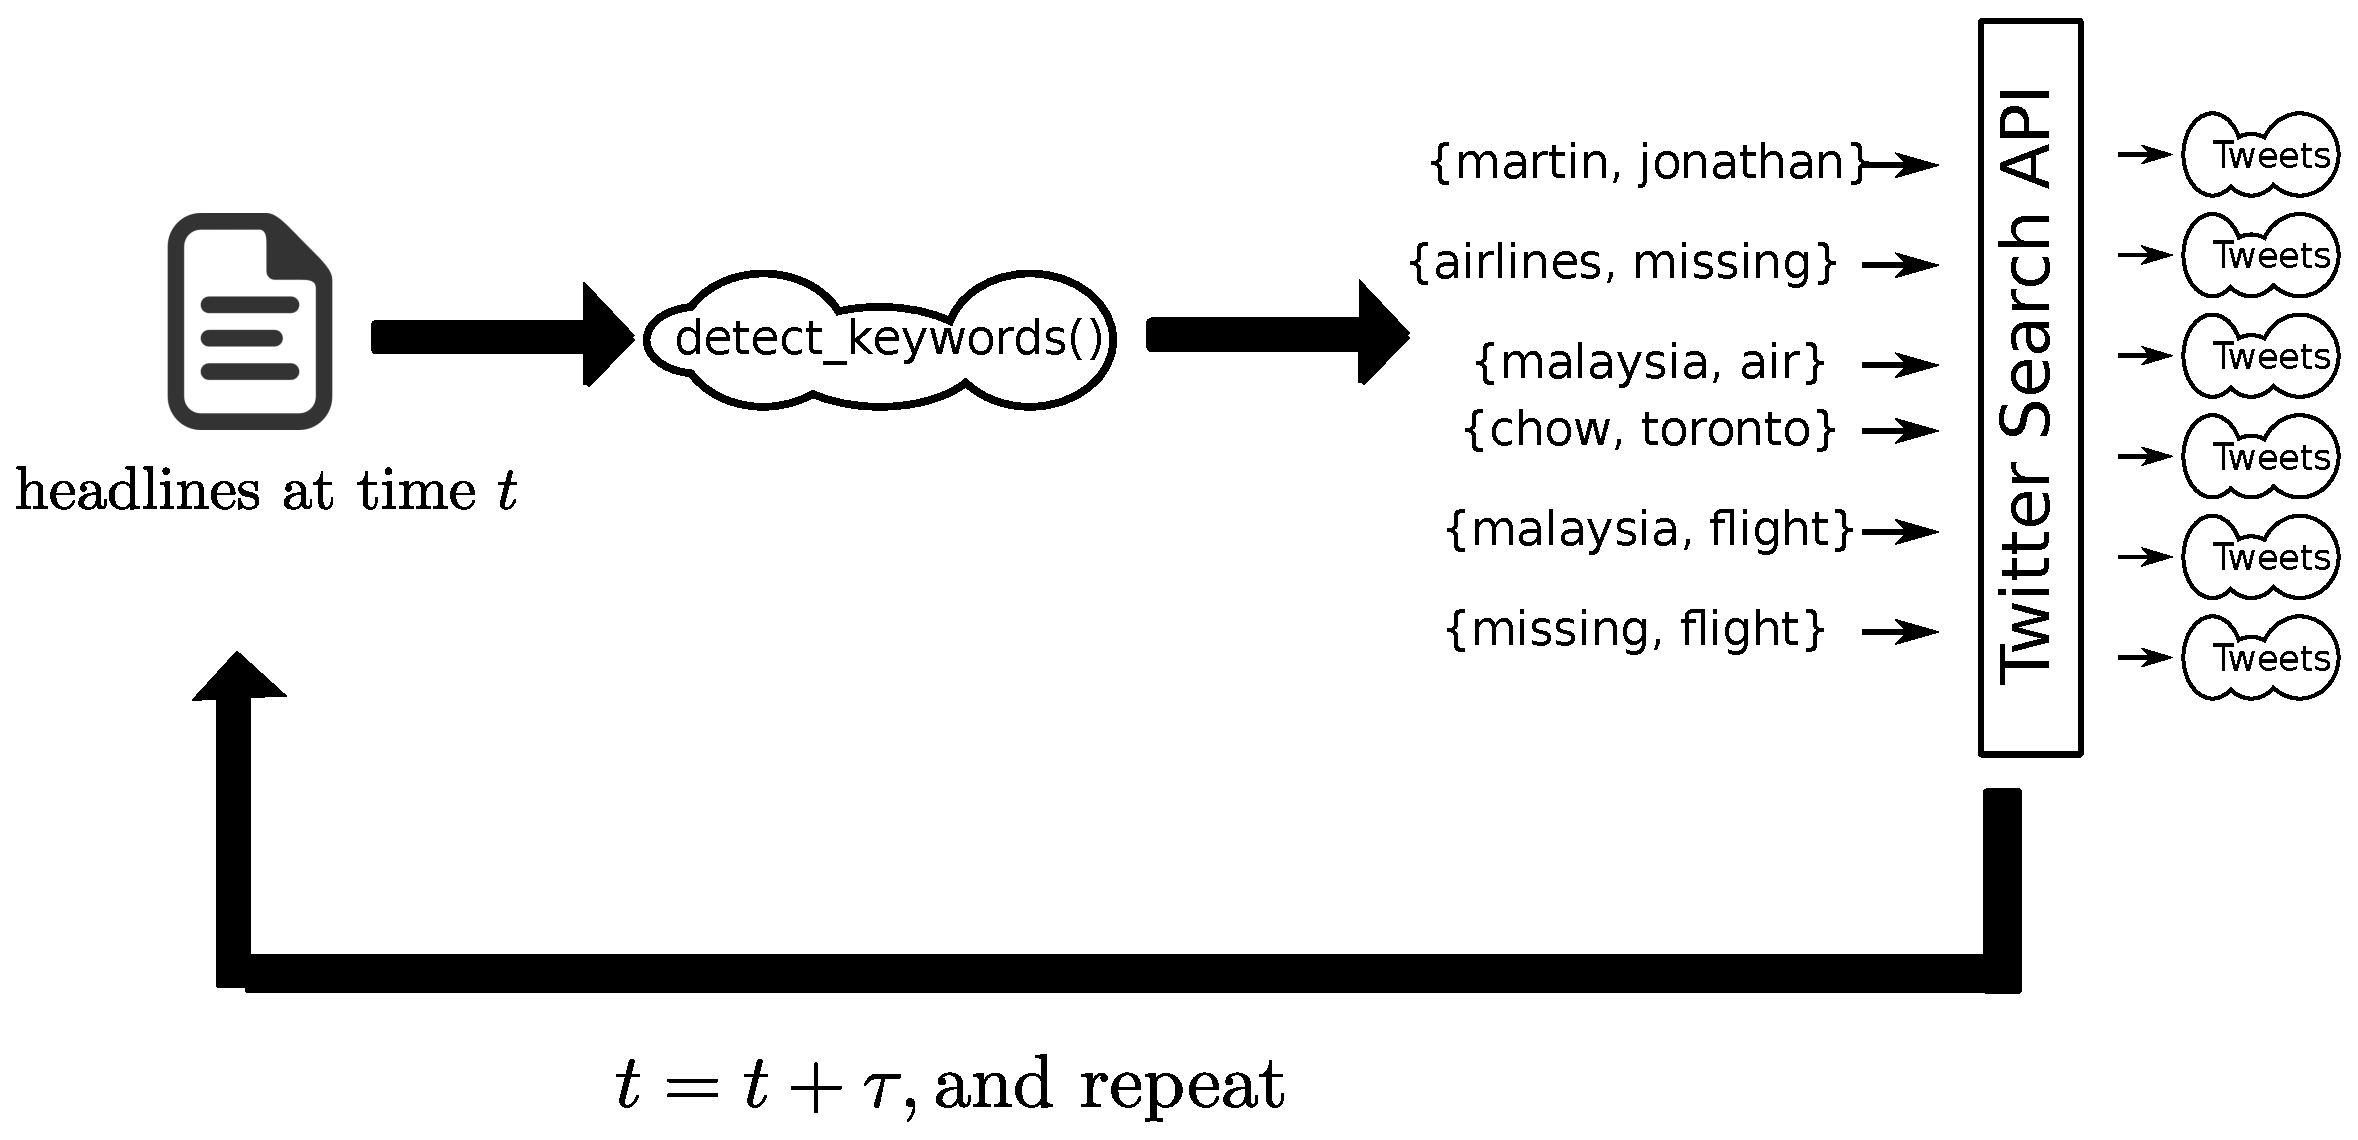
\includegraphics[width=\textwidth]{figures/data/data_collection_1}
\caption[Pipeline of data collection]{Pipeline of data collection. From the
  selected news accounts a set of headlines (tweets) are retrieved. Then, six
  pairs of keywords are identified based on the most frequent itemsets present
  in the headlines. Each pair of keywords is used as a search term of the
  Twitter REST API. For one hour, the process retrieves tweets related to each
  pair of keywords. After that, the process starts again for the next set of
  headlines.}
\label{fig:pipeline}
\end{center}
\end{figure}



Every $t=60$ minutes, all headlines posted in the last $t$ minutes are
retrieved using the API. 
%
We pre-process the retrieved headlines by removing stopwords, punctuation, URLs,
hashtags, mentions, and converting words to lowercase.
%
From the processed headlines the most frequent sets of words are then chosen.
%
From the resulting sets, the top $k=2$ words are chosen from each of the top
$g=6$ groups. 
%
Each pair of words, or keywords, are used as input for the REST API to retrieve
tweets related to the keywords. 
%
The main idea is that if several headlines discuss the same topic, then it is
considered an important topic, and users talk about it using some of the most
frequent words. 
%
We describe the algorithm to identify the frequent
itemsets~\cite{zaki2000scalable} in Algorithm~\ref{alg:detect_keywords}.
%


\renewcommand{\algorithmicrequire}{\textbf{Input:}}
\renewcommand{\algorithmicensure}{\textbf{Output:}}
\newcommand{\I}{\mathcal{I}}
\renewcommand{\G}{\mathcal{G}}
\newcommand{\ess}{\mathcal{S}}

\begin{algorithm}
\caption{Detect common keywords from headlines}
\label{alg:detect_keywords}
\begin{algorithmic}[1]
\REQUIRE A set of $M$ sets of words, $\ess= \{H_1,H_2, \ldots, H_M\}$, positive integers $k, \eta$
\ENSURE $k$ sets of keywords, $G = (\I_1,\I_2,\ldots,\I_{k})$
\STATE $\I_i \leftarrow \emptyset$ for $i = 1,2, \ldots,k$ %\COMMENT{Initialize item sets to empty sets}
\STATE $score_i \leftarrow$ empty dictionary for $i = 1, 2, \ldots,k$ %\COMMENT{Initialize keyword set scores to $1$}
\STATE $i \leftarrow 1$
\FOR{every pair of headlines $\{H_a, H_b\} \in \ess$ such that $|H_a \cap H_b| \geq \eta$}
    \STATE $\G \leftarrow H_a \cap H_b$ \label{alg:line:intersect} %\COMMENT{$\G$ is the set of common words of $H_a$ and $H_b$}
    \STATE $j \leftarrow \operatorname{arg\,max}_j |\I_j \cap \G|$
    \IF{$|\I_j \cap \G| \geq \eta$}
        \STATE $\I_j \leftarrow \I_j \cap \G$
        \STATE $score_{j}[w] \leftarrow score_{j}[w] + 1$ for all $w \in \I_j$
    \ELSE
        \STATE $\I_i \leftarrow \G$
        \STATE $score_{i}[w] \leftarrow 1$ for all $w \in \I_i$
        \STATE $i \leftarrow i + 1$
    \ENDIF
\ENDFOR
\STATE $total\_score_i \leftarrow \sum_{w \in \I_i} score_{i}[w]$ for $i=1,2,\ldots,k$
\RETURN $G = (\I_i$ sorted by $total\_score_i)$

\end{algorithmic}
\end{algorithm}

We only considered the top two keywords from each group, that is, we only
considered pairs of keywords from the headlines. 
%
This is because we use Twitter as our data source, and the tweets can be very
short (140 characters at most at the time of the data collection). 
%
Also, we selected only the top six groups, to obtain an acceptable rate of news
events per time unit. 
%
If there are not enough tweets or groups, we only choose the keywords available
for that period of time.

After one run of the process, a set of $g=6$ \emph{search results} or sets of
tweets are created and stored. 
%
A search is a tuple consisting of a pair of keywords and a set of tweets, each
one of those tweets contains both keywords in its text.

The REST API allows us to get tweets from even before the corresponding headline
was published.
%
The search then continues for about one hour, to get all the related tweets. 
%
If there is a high impact news event, then the users will tweet about it
frequently. 
%
For that reason, the search is performed no more than one hour from the
publication time of the headlines. 
%
Figure~\ref{fig:pipeline} portrays the tweets collection methodology.



\begin{table}
{\small
\begin{center}
\begin{tabular}{lll}
\toprule
 Keywords            &  Date       &  Sample Tweet                                                                                                                                                                                                                     \\
\midrule
 woody allen         &  2014-01-13  &  I love how Woody Allen didn't
 accept his award at the Golden\ldots{} \\
 egypt constitution  &  2014-01-18  &  Egypt passes new constitution\ldots{} \\
 king luther         &  2014-01-20  &  I added a video to a @YouTube
 playlist\ldots{} \\
 brazil world        &  2014-01-26  &  Sports: Hundreds protest against
 World Cup in Brazil: \ldots{} \\
 city chelsea        &  2014-02-15  &  RT@mcfcbuzztap: TEAMtalk FA Cup:
 Manchester City\ldots{} \\
 \bottomrule
\end{tabular}
\end{center}
} \caption[Example of searches.]{Example of searches. The first column
corresponds to the pair of keywords retrieved from the headlines. The second
column corresponds to the date of the search. The last column shows an excerpt
of a tweet in that set.}\label{table:searches}
\end{table}

In summary, the data collection methodology allows for the most recent tweets to
be found on a certain event, assuming that the selected news accounts
consistently post about those events. 
%
The dataset obtained in this phase corresponds to pairs of keywords related to
an event, and a set of tweets that contains the two keywords in its text.
%
Table~\ref{table:searches} shows a few examples of searches.


\subsection{Identifying Events}

We provide some notes about the data collection methodology. 
%
Firstly, there is a temporal sensitivity to the methodology. 
%
For example, one of the keyword pairs obtained as soon the Malaysian airlines
jet disappeared on 2014 was \{plane,missing\}. 
%
Although this keyword pair does not specifically refer to the Malaysian Airlines
jet, it is likely that the tweets retrieved from searching for this pair will
indeed be about the Malaysian Airlines plane that went missing, since the search
is performed as and when the event breaks out. 
%
Secondly, Algorithm~\ref{alg:detect_keywords} may return multiple pairs of
keywords (possibly different pairs) describing the same event. 
%
Some pair examples of keywords produced when there was a bomb threat at Harvard
University in December 2013 were \{harvard, evacuated\}, \{harvard,
explosives\}, etc. 
%
How do we merge the keyword pairs which belong to the same event? 
%
In order to address this, we collect all the pairs obtained in the past $24$
hours, and build a graph with keywords as nodes, and keyword pairs (as obtained
from Algorithm {\ref{alg:detect_keywords}}) as edges (see
Figure~\ref{fig:connected-component}). 
%
We then discover the connected components of this graph, and treat each
connected component as an ``event". 
%



\begin{table}

\begin{center}
\begin{tabular}{lllll}
\toprule
  Keywords              &  Date and time     &     &  Keywords              &  Date and time     \\
\midrule
 bill aid              &  2014-04-02 00:00  &     &  quake chile           &  2014-04-02 03:00  \\
 island refinery       &  2014-04-02 00:00  &     &  earthquake magnitude  &  2014-04-02 03:00  \\
 congress ukraine      &  2014-04-02 00:00  &     &  chile tsunami         &  2014-04-02 03:00  \\
 earthquake struck     &  2014-04-02 01:00  &     &  iquique chile         &  2014-04-02 03:00  \\
 tsunami chile         &  2014-04-02 01:00  &     &  chile five            &  2014-04-02 05:00  \\
 magnitude earthquake  &  2014-04-02 01:00  &     &  earthquake magnitude  &  2014-04-02 04:00  \\
 tsunami chile         &  2014-04-02 01:00  &     &  chile earthquake      &  2014-04-02 05:00  \\
 watches tsunami       &  2014-04-02 01:00  &     &  gray primary          &  2014-04-02 05:00  \\
 chile tsunami         &  2014-04-02 02:00  &     &  warning tsunami       &  2014-04-02 05:00  \\
 earthquake tsunami    &  2014-04-02 02:00  &     &  earthquake chile      &  2014-04-02 04:00  \\
 tsunami chile         &  2014-04-02 02:00  &     &  hawaii advisory       &  2014-04-02 05:00  \\
\bottomrule
\end{tabular}
\end{center}
\caption[Example pairs of keywords from April 2nd, 2014.]{Some pairs of
  keywords from April 2nd, 2014. Several keywords are related to an
  earthquake and tsunami occurred on Iquique, Chile that day. (The
  times are in UTC.)}\label{table:example-pairs}
\end{table}


For example, Table~\ref{table:example-pairs} demonstrates some of the keywords
detected on April 2nd, 2014. 
%
Several of them contain the word ``earthquake'', ``tsunami'' or ``chile''.
%
Indeed, on that day an earthquake struck and was followed by a tsunami on the
coast of Iquique and Arica, in Chile. 
%
The occurrence of several pairs of keywords related to the same event is a
consequence of the news accounts posting several headlines about that event, in
different times. 
%
The tweets about the event did not last one hour, but instead several. 
%
For that reason, it is necessary to group similar pairs of keywords to form
events.
%
See Table~\ref{table:example-events} for example events retrieved.


\begin{table}
\begin{center}
\begin{tabular}{rl}
\toprule
 Keywords  &  Event                                                                        \\
\midrule
       16  &  chile, northern, iquique, panama, fires, watches, coast, canceled, tsunami,  \\
           &  five, quake, following, struck, warning, earthquake, magnitude               \\
       11  &  europe, jobs, clegg, 191, tonight, nick, won, farage, nigel, farage, round   \\
        9  &  passengers, police, scene, four, incident, details, active, hood, fort       \\
        4  &  wall, prime, school, edinburgh                                               \\
        3  &  modi, narendra, buxar                                                        \\
        2  &  paul, cosford                                                                \\
        2  &  interior, ministry                                                           \\
        2  &  president, bachelet                                                          \\
        2  &  firetv, amazon                                                               \\
\bottomrule
\end{tabular}
\end{center}

\caption[Some events identified from April 2nd, 2014.]{Some events
  identified from April 2nd, 
  2014. The largest event corresponds to the earthquake in Chile. They
  are sorted on the number of keywords.}\label{table:example-events}
\end{table}

\begin{figure}
    \centering
    \includegraphics[width=.6\textwidth]{figures/data/connected_components.eps}
    \caption[Example of connected components]
    {Example of connected components. Two keyword sets are joined if they share
    at least one keyword in common.}\label{fig:connected-component}
\end{figure}



\section{Data Cleaning and Validation}\label{sec:cleaning}

There are two issues in our methodology: domain-specific stopwords and very old
tweets.

First, the event identification methodology does not take into account the use
of common words in the headlines. 
%
After removing the typical stopwords (words like ``the'', ``is'', ``do'', etc.),
some other common words appear in the headlines. 
%
Those words can be selected as the keywords for some news events, and by being
common, can join unrelated events together.
%
For example, words like ``update'' or ``breaking'' are commonly used by
different news sources. 
%
We validated our methodology by comparing the resulting events with random
events, those resulting from joining random keyword sets.

Second, due to the REST API behavior, some tweets are very old with respect to
the corresponding event. 
%
Sometimes the tweets are months or even years old. 
%
For that reason, we remove all tweets that were more than ten days old from the
date of the event. 

The event durations are then analyzed in order to verify if including the first
portion of the data, for each news event, makes sense in terms of their
duration. 
%
For instance, if the tweets are evenly distributed, the time span in the first
5\% of the total amount of tweets should be half the duration of the first 10\%,
one quarter of the 20\%, and so on. 
%
However, our data shows that, for example, the first few tweets of an event are
from two or more years previous to the occurrence, and the remaining tweets are
mainly concentrated closely around the date of the event.
%
The first 5\% of the tweets would then be significantly older than the rest
95\% in terms of time duration of the event. 


\subsection{Detecting Articulation Words}

A problem that arose during the data collection was that, sometimes unrelated
events were joined together with keywords that was common to both events.  
%
This happens when two or more headlines from different events share a common
keyword. 
%
We performed a simple approach to identify such words and remove them from the
process.

Typical stopwords were removed when detecting groups of keywords to perform
searches, but some other words were common among the news accounts queried. 
%
For example, words like ``watch'', ``live'', or ``update'' are common to express
things like ``watch this video'', ``we are live on TV'', or to update a previous
headline with more info about it. 
%
By being common to different events (for example: ``Watch Jim Harbaugh's press
conference
live''\footnote{\url{https://twitter.com/49ers/status/519202023628374016}
(Accessed: February 29, 2020)}  and ``WATCH LIVE: Of the 48 people being
monitored for contact with Dallas patient, no one is showing any
symptoms''\footnote{\url{https://twitter.com/PzFeed/status/519203692898435072}
(Accessed: February 29, 2020)}), they can end up in unrelated events by joining
the keywords by those stopwords.


One approach to dealing with this problem is to have a pre-defined list of
stopwords to remove from the stream of headlines. 
%
Although we do not know beforehand which words those are. 
%
We call such words \emph{articulation words} in the sense that if they appear as
keywords after processing a group of headlines, then when joining the searches
together, those words would join unrelated events. 

%%

Intuitively, if a word appears in all the documents, then its {\em
tf-idf}~\cite{sparck1972statistical} score is generally low in all the
documents.  
%
However, if the word appears in very few documents, its statistic in those
documents is fairly high, indicating that the word is somehow representative of
the content of the document. 
%
It turns out the articulation words do not occur often enough for them to be
detected by regular \emph{tf-idf}, but do occur enough times for them to falsely
relate several unrelated events together. 
%
To identify a group of those keywords, we used a modified \emph{tf-idf} to
detect them from the headlines.

The modified version of \emph{tf-idf}, what we refer to as \emph{maxtf-idf}, is
meant to assign more weight to the terms that are frequent in any document. 
%
For instance, \emph{tf-idf} of a term in a document tries to assign a weight
related to how ``rare'' that term is in the whole collection, and how frequent
it is in that document, by indicating how representative the term is with
respect to the document. 
%
On the other hand, what we want to achieve is to weigh a term more if it
is more frequent in any document, relative to the frequency in the current
document. 
%
With that in mind, we want to identify terms that might be ``adding noise'' to
the corpus, and hence, to join unrelated events together.

The definition of \emph{maxtf} is as follows:

\begin{equation}
\text{maxtf}(t,\mathit{d},D) = 0.5 + \frac{0.5 + max\{f(t,\mathit{d}') : \mathit{d}' \in D\}}{max\{f(w,\mathit{d}) : w \in \mathit{d}\}}
\end{equation}

and for \emph{idf}, the usual formula:

\begin{equation}
\text{idf}(t,D) = \log\frac{N}{|\{\mathit{d} \in D : t \in \mathit{d}\}|}
\end{equation}

\noindent where $t$ is a term, $\mathit{d}$ is a document, and $D$ is the corpus
of documents. 
%
In this case, we set $t$ as a keyword, $\mathit{d}$ as the set of keywords of
one hour, and $D$ the set of documents of that day.

\begin{figure}
\begin{center}
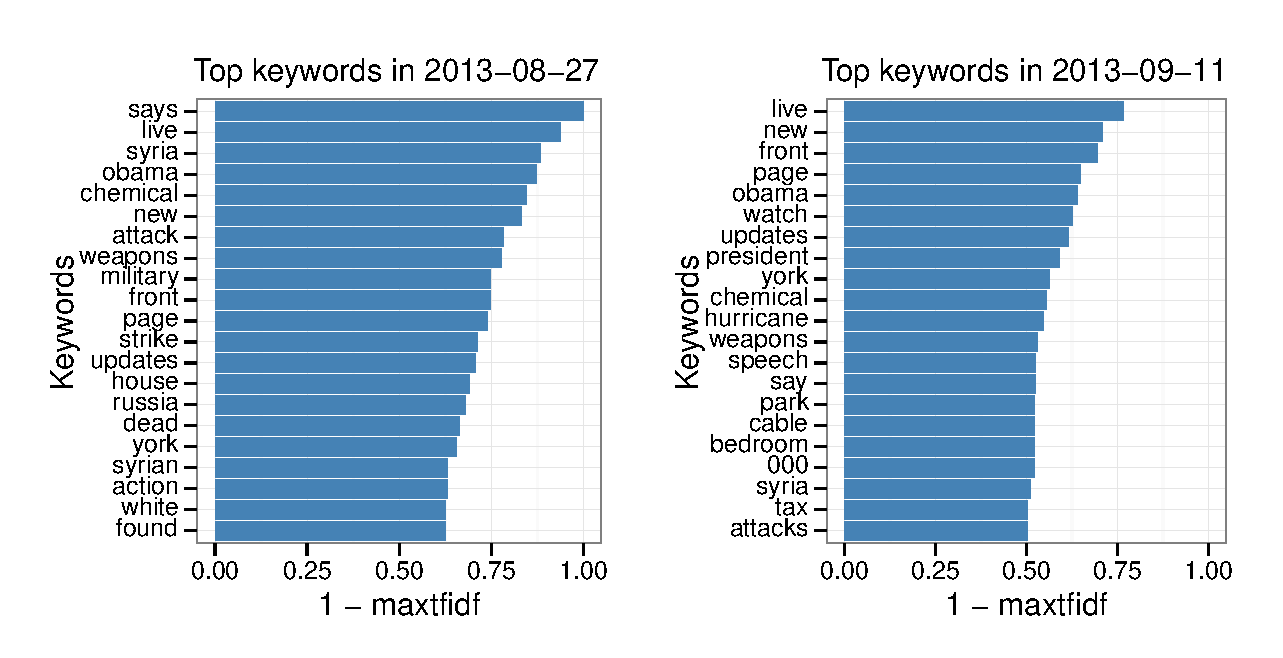
\includegraphics[width=\textwidth]{figures/data/stopwords}
\caption[Stopwords detection.]{Stopwords detection. Normalized
  $1-\text{maxtf-idf}$ score for data from August 27th (left) and August 28th
  (right) of 2013. The top score words for both plots are ``says'' and ``live''.
  We used the top score words to disconnect connected components of events. The
  title indicates the date when those keywords were identified, while the number
  beside corresponds to the total number of keywords.}
\label{fig:stopwords}
\end{center}
\end{figure}


After identifying such words, the idea was to disconnect the components
connected by those words. 
%
The process was to disconnect each component by the word with top normalized
$1-\text{maxtf-idf}$ score each time until the component could not be
disconnected further. 
%
We ended by adding the top score words to a list of banned words which were
ignored from subsequent runs of the data collection methodology. 
%
In Figure~\ref{fig:stopwords} there are two examples of this process to identify
the words.


\subsection{Validation of Event Modeling}\label{sub:valcoll}

In order to validate the results of the event identification process, we
compared our results with a baseline consisting on randomly generated events.

We generated artificially connected components taking randomly searches from the
first stage, and then merging their tweets to generate a ``random'' connected
component. 
%
The assumption here is that the tweets of a search are closely related to its
pair of keywords. 
%
From that, we wanted to ensure that the identified events make sense by
comparing them with random components. 
%
The idea is that using the connected components approach would join related
events together, so it would suffice to compare to a random baseline.

\begin{figure}
\begin{center}
\includegraphics[width=.8\textwidth]{figures/data/connected_components_validation2.pdf}
\caption[Validation of connected components] {Validation of connected
  components. Each plot in this figure compares the quality of the cluster of
  tweets obtained from connected components and random components. The blue line
  corresponds to our approach, while the red line corresponds to the random
  components baseline. For visual clarity, the values obtained from connected
  components were sorted in ascending order, hence the blue line is
  monotonically increasing. The values obtained were rearranged in the same
  order as well.}\label{fig:connected_components_validation} 
\end{center}
\end{figure}

\begin{table}
\centering
\begin{tabular}{| c | c | c |}
\hline
Name & Metric & Meaning \\
\hline
\hline
$I_1$ & $\sum_{i=1}^k \frac{1}{n_i} \sum_{(u,v) \in S_i} \text{sim}(u,v)$ & Higher value is better\\
\hline
$I_2$ & $\sum_{i=1}^k \sqrt{ \sum_{(u,v) \in S_i} \text{sim}(u,v)}$ & Higher value is better \\
\hline
$E_1$ & $\sum_{i=1}^{k} n_i \frac{\sum_{v \in S_i, u \in S} \text{sim}(u,v)}{\sqrt{\sum_{(u,v) \in S_i} \text{sim}(u,v)}}$ & Lower value is better \\
\hline
$G_1$ & $\sum_{i=1}^k \frac{\sum_{v \in S_i, u \in S}\text{sim}(u,v)}{\sum_{(v,u) \in S}\text{sim}(v,u)}$ & Lower value is better \\
\hline
$G_1^{'}$ & $\sum_{i=1}^k n_i^2 \frac{\sum_{v \in S_i, u \in S}\text{sim}(v,u)}{\sum_{(u,v) \in S_i}\text{sim}(u,v)}$ & Lower value is better \\
\hline
$H_1$ & $\frac{I_1}{E_1}$ & Higher value is better \\
\hline
$H_2$ & $\frac{I_2}{E_1}$ & Higher value is better \\
\hline
\end{tabular}
\caption[Clustering metrics used for validation]{Clustering metrics used for
  validation. This table lists the clustering metrics used in Figure
  \ref{fig:connected_components_validation}. Those formulas correspond to usual
  clustering evaluation metrics, like inter-cluster similarity ($I_1, I_2$),
  intra-cluster similarity ($E_1, G_1, G_1'$) and similarity radio ($H_1, H_2$).
  In $I_1, I_2, H_1, H_2$ a higher value is better.  In $G_1, G_1^{'}$, lower
  value is better. }
\label{table:clustering_metrics}
\end{table}

We calculated standard internal clustering metrics~\cite{zhao2001criterion}
(listed in Table~\ref{table:clustering_metrics}) over the components and on the
random components and then compare their results. 
%
The comparisons were made by taking components of the same size (in terms of
keywords and tweets, taking samples of tweets). 
%
Essentially, considering a component as a cluster, the metrics evaluate the
similarity intra- and inter-clusters. 
%
We compare the metrics against random clusters to see if our approach tends to
join related events together, compared to a baseline.
%
Equal results mean that our approach is no better than joining searches
randomly. 
%
The results by metric are shown in
Figure~\ref{fig:connected_components_validation}. For almost every metric, our
approach is better than random.


\subsection{Event duration}\label{sub:dur}

Due to the capabilities of the REST API, the tweets collected can be older than
the actual date of the event detected. 
%
For that reason, some tweets can be very old and not relevant to the event
itself. 
%
Furthermore, when a retweet is collected by the process, also the original tweet
is stored\footnote{The data of the original tweet is included in the data of the
retweet}. 
%
This could be a problem especially when we want to perform predictions using the
first part of the data. 


\begin{figure}
\centering
\includegraphics[width=\textwidth]{figures/data/duration-differences.pdf}
\caption[Duration differences of events.]{Duration differences of events. The
  $x$-axis represents the categories of datasets: the first one (t5\%-t0)
  represents the difference of time between the timestamp of the oldest tweet
  and the newest tweet on the first 5\% of the tweets. The next one (t10\%-t5\%)
  corresponds to the difference between the newest tweet in the first 10\% and
  the newest tweet on the first 5\% of data, etc. After removing the first 5\%
  of data, the time differences are roughly the same across all
  datasets.}\label{fig:duration-differences}

\end{figure}

After collecting tweets for an event, we remove the first 5\% of tweets of each
event, in addition to restrict tweets of an event up to ten days before the day
of its publication. 
%
We saw that the first 5\% of the tweets cover the largest amount of time on all
events, due to the problems exposed above. 
%
After removing the first 5\%, the events duration were more consistent (the
first 10\% covers twice the amount of time that the first 5\% covers, and so
on). 
%
Figure~\ref{fig:duration-differences} shows the effect of removing the first 5\%
of data by calculating the time differences between the timestamps of the tweets
at the ends of each dataset.


\begin{figure}[t]
  \centering
  \begin{subfigure}{\textwidth}
    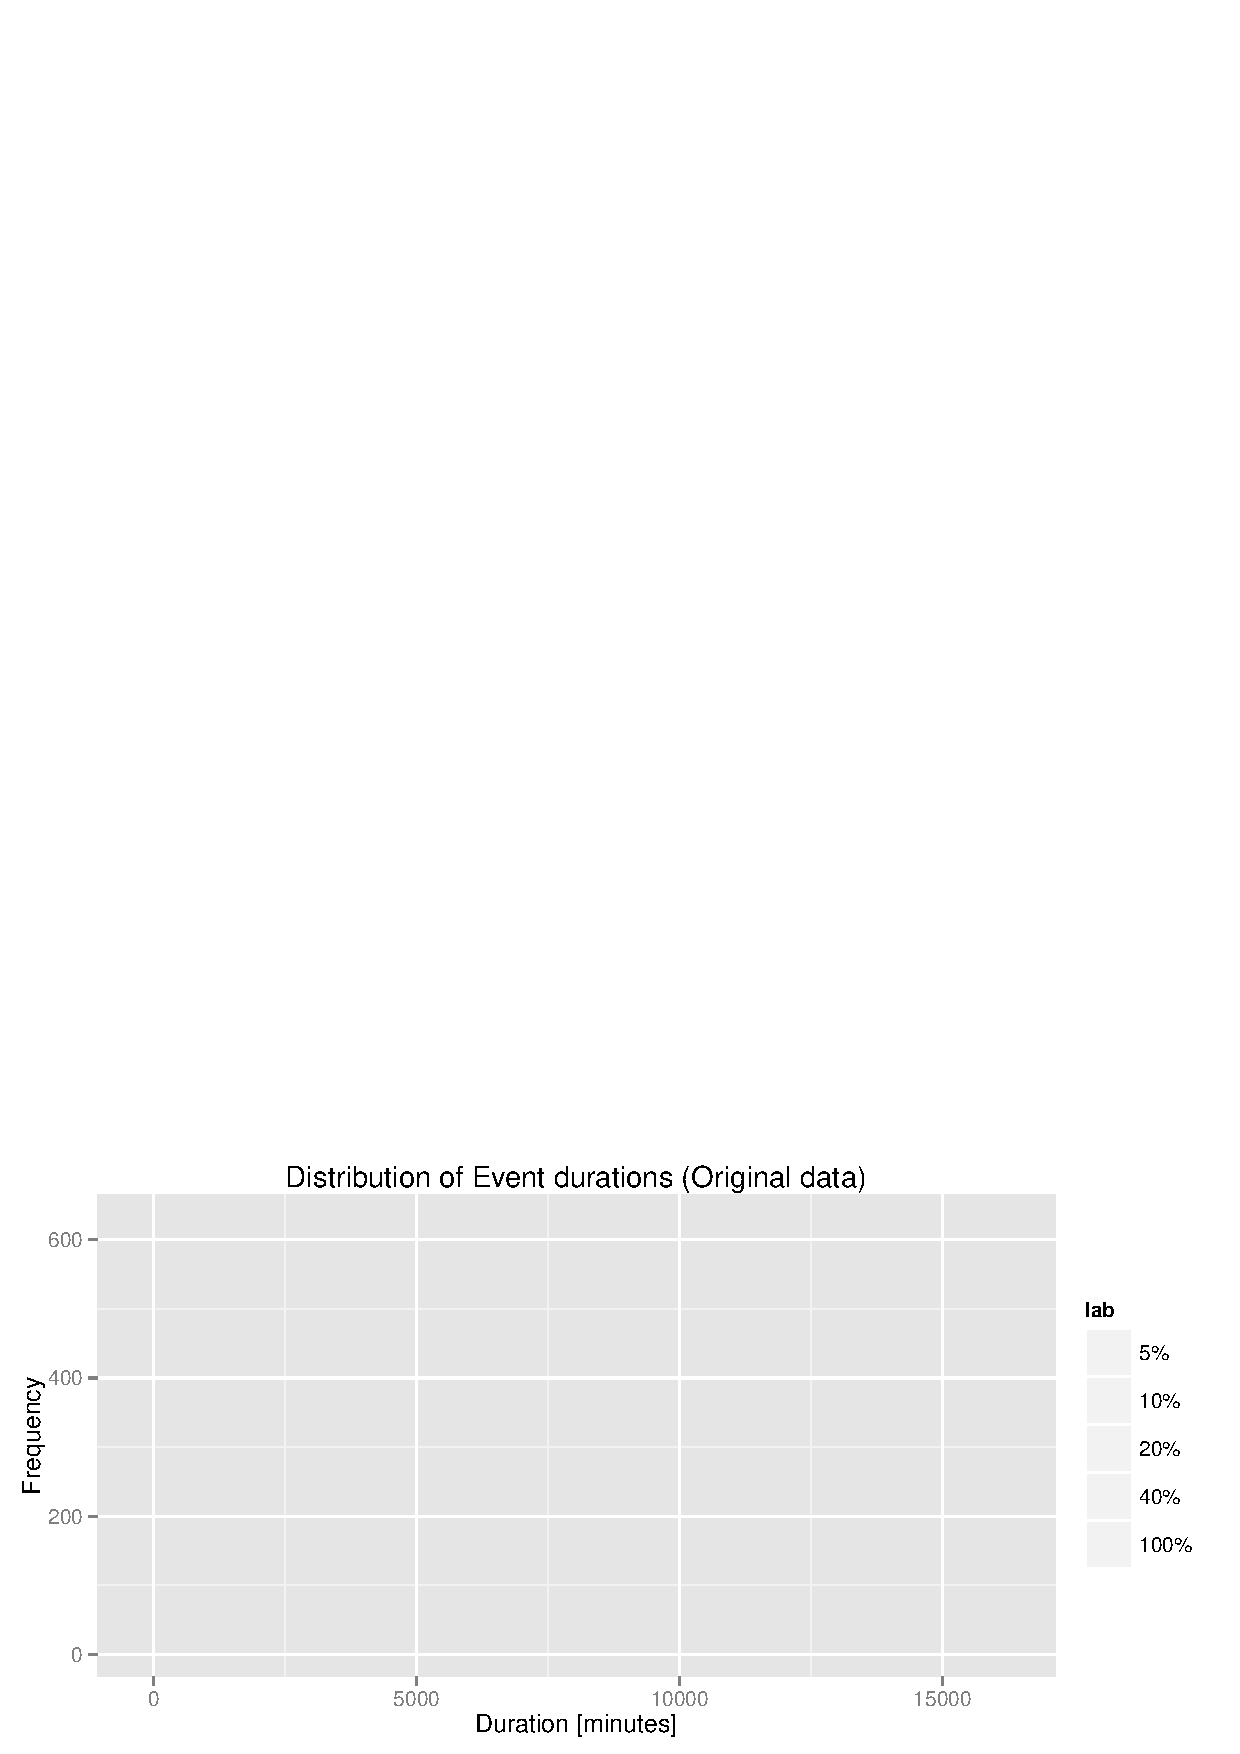
\includegraphics[width=\textwidth]{figures/data/dist-events-durations-o.pdf}
    \caption[Distribution of event duration on the original
      dataset.]{Distribution of event duration on the original dataset.} 
    \label{sfig:dist-events-durations-o}
  \end{subfigure}

  \begin{subfigure}{\textwidth}
    \centering
    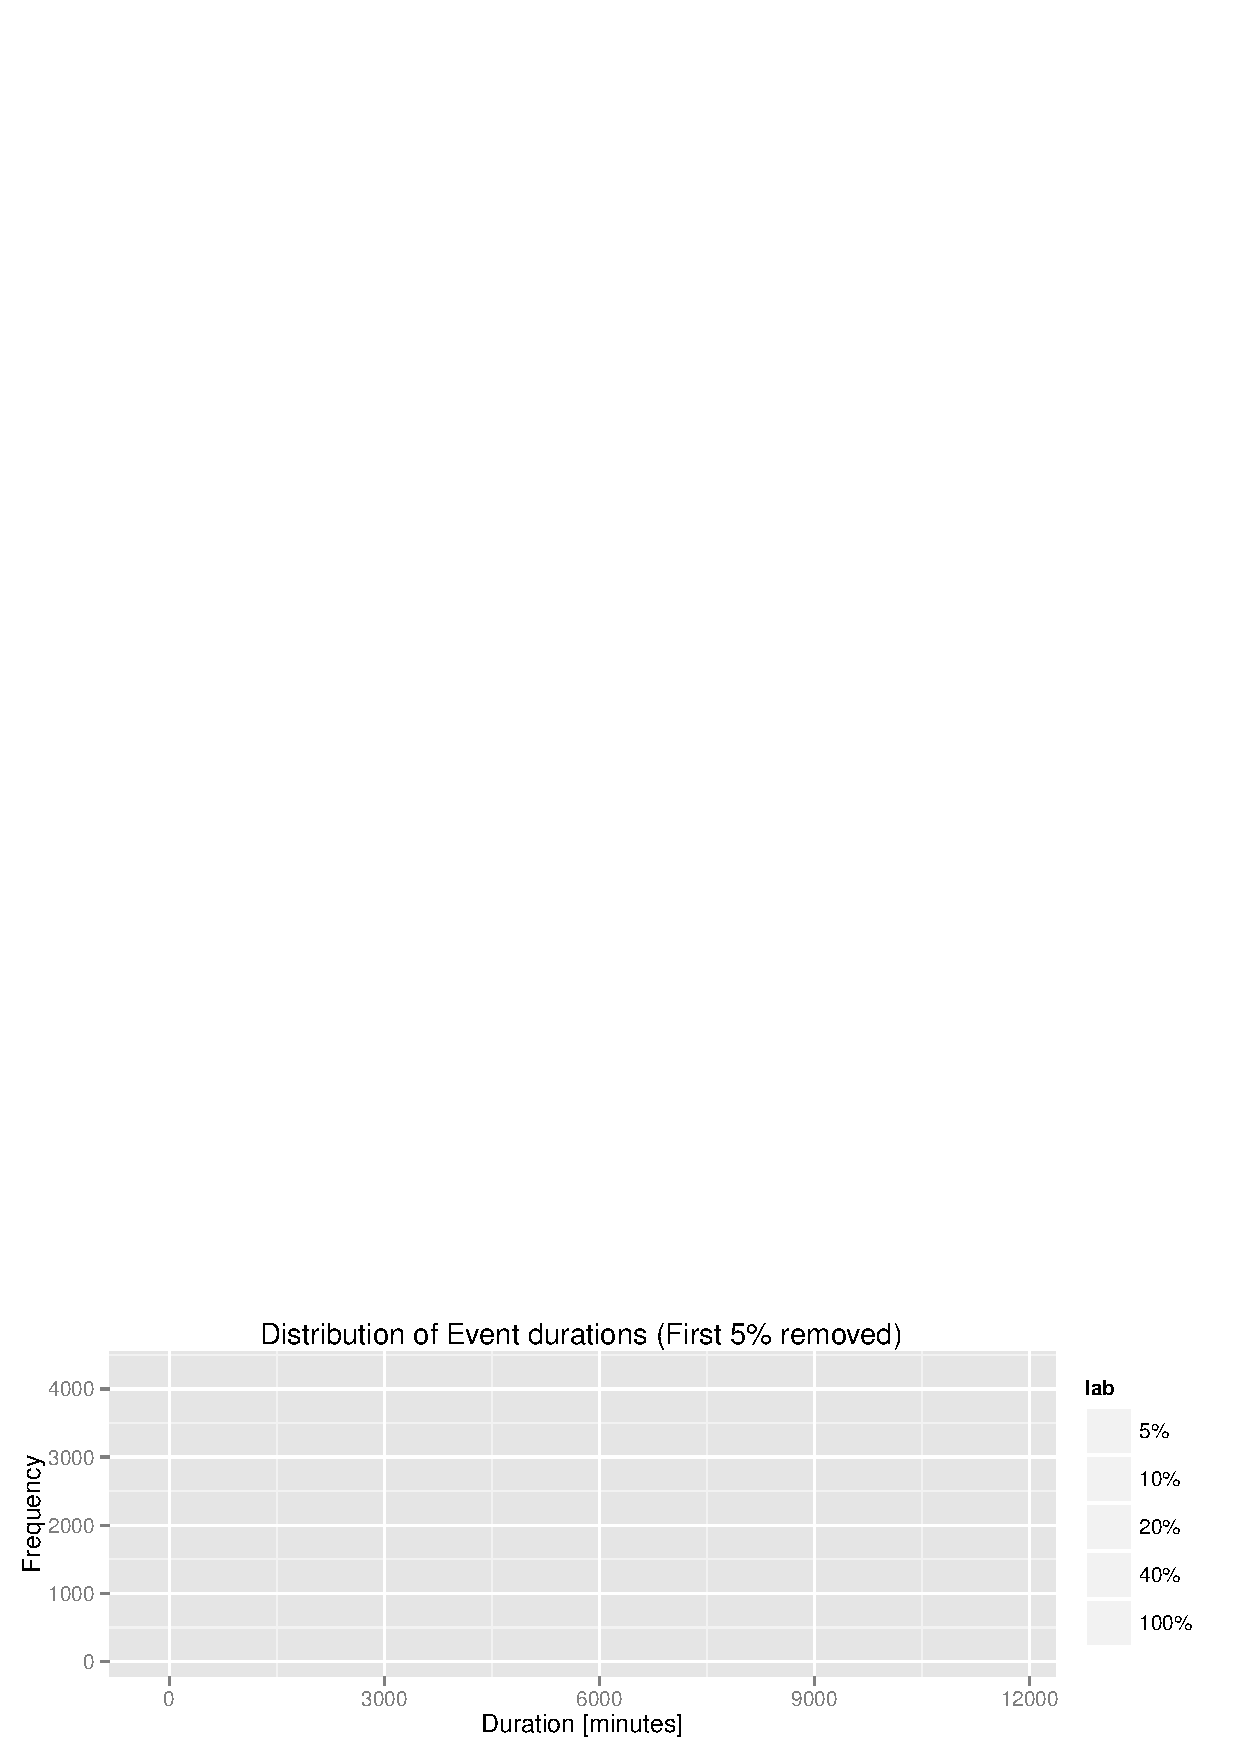
\includegraphics[width=\textwidth]{figures/data/dist-events-durations-5.pdf}
    \caption[Distribution of event duration on the 5\%-trimmed
      dataset.]{Distribution of event duration on the 5\%-trimmed dataset.} 
    \label{sfig:dist-events-durations-5}
  \end{subfigure}

  \caption[Distribution of event duration]{Distribution of event duration. In
    (a) we see that there is a non-negligible amount of events with a
    high duration (between 7 and 10 days). In (b), we see a clearer power law on
    the distribution of events after removing the first 5\% of tweets.}
  \label{fig:dist-events-durations}
\end{figure}

Event duration distributions are shown in
Figure~\ref{fig:dist-events-durations}. 
%
Figure~\ref{sfig:dist-events-durations-o} shows that there is a non-negligible
amount of events with a duration between 7 and 10 days. 
%
By considering the first 5\% of tweets from those events, the oldest tweets will
correspond to situations when the event has not already happened yet, and it
will lead to errors or incorrect results. 
%
Removing the first 5\% produces a cleaner dataset, as shown in
Figure~\ref{sfig:dist-events-durations-5}.


%%%
\paragraph{Summary.}
%
Our data collection methodology consisted of a pipeline starting at headline
retrieval from manually selected news sources, ending with event identification.

An event is a set of keywords with a set of tweets that talk about these
keywords.
%
The keywords can be seen as the event representatives. 
%
For example, the event \{chile, northern, iquique, tsunami, struck, warning,
earthquake, magnitude\} describes an earthquake that occurred in Chile on April
2th. 
%
However, a few challenges had to be addressed from this methodology.

Some keywords are common across several distinct events. 
%
For that reason, it was necessary to identify such words and remove them from
the keywords detection phase, for example, words like ``update'', ``watch'', or
``live'', which do not add any value to the meaning of any event. 

Finally, due to the nature of the methodology proposed, the tweet sets had to be
trimmed because of their long duration. 
%
Because of the Twitter REST API, sometimes tweets from long ago were retrieved,
but since they add only noise to our dataset, they were removed.


\chapter{User Reaction: Predicting and Characterizing High-Activity News Events} 
\label{chapter:high-activity}

\section*{Abstract}


On-line social networks publish information on a high volume of real-world
events almost instantly, becoming a primary source for breaking news.  
%
Some of these real-world events can end up having a very strong impact on
on-line social networks.  
%
The effect of such events can be analyzed from several perspectives, one of them
being the intensity and characteristics of the collective activity that it
produces in the social platform. 
%
We research 5,234 real-world news events encompassing 43 million messages
discussed on the Twitter microblogging service for approximately 1 year.  
%
We show empirically that exogenous news events naturally create collective
patterns of bursty behavior in combination with long periods of inactivity in
the network. 
%
This type of behavior agrees with other patterns previously observed in other
types of natural collective phenomena, as well as in individual human
communications. 
%
In addition, we propose a methodology to classify news events according to the
different levels of intensity in activity that they produce. 
%
In particular, we analyze the most highly active events and observe a consistent
and strikingly different collective reaction from users when they are exposed to
such events. 
%
This reaction is independent of an event's reach and scope.  
%
We further observe that extremely high-activity events have characteristics that
are quite distinguishable at the beginning stages of their outbreak.  
%
This allows us to predict with high precision, the top 8\% of events that will
have the most impact in the social network by just using the first 5\% of the
information of an event's lifetime evolution. 
%
This strongly implies that high-activity events are naturally prioritized
collectively by the social network, engaging users early on, way before they are
brought to the mainstream audience.


\section*{Introduction}
% Motivation

Social media can be considered a primary source of breaking news information for
millions of users all over the world~\cite{Kwak:2010}.\todo[inline]{more recent refs}
%
Social media along with mobile internet devices have crowdsourced the
task of disseminating real-time information. 
%
As a result, both news media and news consumers have become inundated with much
more information than they can process. 
%
One possible way of handling this data overload, is to find ways to filter and
prioritize information that has the potential of creating a strong collective
impact. 
%
Understanding and quickly identifying the type of reaction that certain
exogenous events will produce in social media, at both global and
local scales, can help in the understanding of collective human behavior.
%
This may as well as improve information delivery, journalistic coverage and
crisis management, among other things. 
%
We address this challenge by analyzing the properties of real-world news events
in social media, showing that they corroborate patterns previously identified in
other case studies of human communications. 
%
In addition, we present our main findings of how news events that produce
extremely high-activity can be clearly identified in the early stages of their
outbreak.

% Brief background on the problem

The study of information propagation on the Web has sparked tremendous interest
in recent years. 
%
Current literature on the subject primarily considers the process through which
a {\em meme}, usually a piece of media (like a video, an image, or a specific
Web article), gains popularity
\cite{Castillo:2014,Szabo:2010,Lerman:2010,Tatar2014,Pinto:2013,Ahmed:2013,Li:2016:concept:drift,
Liu:2015:UN}. 
%
However, a meme represents a simple information unit and its propagation
behavior does not necessarily correspond to that of more complex information
such as news events. 
%
News events are usually diffused in the network in many different formats, e.g.,
a particular news story such as an {\em earthquake in Japan} can be communicated
through images, URLs, tweets, videos, etc. 
%
Therefore, current research can benefit from analyzing the effects of more
high-level forms of information. 

Traditionally, the impact of information in on-line social networks has been
measured in relation to the total amount of attention that this subject receives
\cite{berger2012makes,iribarren2011branching,guerini2011exploring,mills2012virality,gaugaz2012predicting}.
%
That is, if a content posted in the network receives votes/comments/shares above
a certain threshold it is usually deemed as {\em viral} or {\em popular}.
%
Nevertheless, this notion of popularity or impact will favor only information
that produces very large volumes of social media messages. 
%
Naturally, global breaking news that has world-wide coverage and that produces a
high volume of activity in a short time should be considered as having a strong
impact on the network.  
%
However, there are other types of events that can produce a similar reaction in
smaller on-line communities such as, for example, on users from a particular
country (e.g., the withdrawal of the main right wing presidential candidate in
Chile due to psychiatric problems, just before
elections~\cite{chile_elections}). 
%
Clearly, events of local scope do not produce as much social media activity as
events of global scope, but they can create a strong and immediate reaction from
users in local networks \cite{ReisBOPKA15}. 
%
Conversely, there are large events which do not produce an intense reaction,
such as {\em The Oscars} (Fig~\ref{fig:fig1}), which span a long period of time
and are discussed by social network users for weeks or even months, but do not
spark intense user activity. 
%
Therefore, it is reasonable to consider additional dimensions, than just volume,
when analyzing the impact of information in on-line communities.  

Prior research has shown that certain types of individual activities, such as
communications (studied in email exchanges), work patterns and entertainment,
follow a behavior of bursts of rapidly occurring actions followed by long
periods of inactivity~\cite{barabasi2005origin}, referred to as {temporally
inhomogeneous} behavior~\cite{karsai2012universal}.  
%
This type of behavior initially observed in individual activities, has also been
observed in relation to other naturally occurring types of collective phenomena
in human dynamics similar to processes seen in self-organized
criticality~\cite{karsai2012universal}.  
%
In particular, extremely high-activity bursty behavior seems to also occur in
critical situations, observed from the information flow in cell phone networks
during emergencies\cite{gao2014quantifying}.  
%
Although, there is research towards modeling this type of collective behavior
\cite{yan2013information} in on-line social networks, to the best of our
knowledge, it has not yet been analyzed quantitatively.





% when
% consulting journalists on how news media sources measure the impact of
% news, we learn that they too face the issue of not having a clear way
% to approach this problem.

% Our contributions

%\newtext{

Our work focuses on high-activity events in social media produced by real-world
news, with the following contributions:
\begin{enumerate}

\item We introduce a methodology for modeling and classifying events in social
media, based on the intensity of the activity that they produce. 
%
This methodology is independent of the size and scope of the event, and is an
indicator of the impact that the event information had on the social network.

\item We show empirically that real-world news events produce collective
patterns of bursty behavior in the social network, in combination with long periods of
inactivity. 
%
Furthermore, we identify events for which most of their activity is concentrated
into very high-activity periods, we call these events {\em high-activity
events}.

\item We determine the existence of unique characteristics that differentiate
how high-activity events propagate in the social network.

\item We show that an important portion of high-activity events can be predicted
very early in their lifecycle, indicating that this type of information is
spontaneously identified and filtered collectively, early on, by social network
users.

\end{enumerate}
%}

%We focus on high-impact news events in social media, contributing by (i)
%\textcolor{blue}{defining a new concise way for measuring information impact that
%is independent of the size (whether large or small) and scope (whether
%local or global) of the event, but is representative of the urgency
%and immediacy of the reaction of users on the social media} (ii)
%determining the existence of unique characteristics that differentiate
%how high-impact exogenous events are propagated in the network, and
%(iii) show, through the creation of an early prediction model for
%high-impact events, that these types of news events are naturally
%identified and filtered by the network at very early stages of their
%outbreak.
\section*{Materials and Methods}

% model
We define an event as a conglomerate of information that encompasses
all of the social media content related to a real-world news
occurrence. Using this specification, which considers an event as a
complex unit of information, we measure the impact produced by an
event in terms of the strength or immediacy of the social network's
reaction to its information.  In particular, we measure an event's
impact using the \emph{arrival time intervals} between consecutive
social media messages in the event itself.
% The \emph{distribution} of the arrival time intervals is studied for
% a given event.
In those terms, we consider high-impact events to be those for which
the \emph{distribution} of arrival time intervals is most heavily
skewed towards the smallest possible interval, zero. In other words,
events for which most messages arrive in almost instant successions
are defined as high-impact.
%For example, Fig.~\ref{fig:example_buzz}
%shows the distribution of arrival time intervals for two events: {\em
%  (a) The death of Nelson Mandela} and {\em (b) The Oscars}. In this
%example,
For instance, we can observe that the majority of the messages about
the death of political leader Nelson Mandela
(Fig.~\ref{fig:nelson_mandela}) arrived within almost zero seconds of
each other. On the contrary, the messages about The Oscars
(Fig.~\ref{fig:oscars}) are much more spread out in time.
\begin{figure}
  \centering
  \begin{subfigure}{\textwidth}
    %\includegraphics[width=\textwidth]{figures/nelson_mandela_buzz_example}
    \caption{User posts about the death of Nelson Mandela arrive
      almost instantly.}
    \label{fig:nelson_mandela}
  \end{subfigure}%

  ~ %add desired spacing between images, e. g. ~, \quad, \qquad, \hfill etc.
  % (or a blank line to force the subfigure onto a new line)
  \begin{subfigure}{\textwidth}
    %\includegraphics[width=\textwidth]{figures/may_oscar_buzz_example}
    \caption{User posts about The Oscars arriving several weeks before
      the event.}
    \label{fig:oscars}
  \end{subfigure}%
  ~ %add desired spacing between images, e. g. ~, \quad, \qquad, \hfill etc.
  % (or a blank line to force the subfigure onto a new line)

  \caption{\textbf{Illustrative examples of two events
      summarized by our method. The event [nelson, mandela] (\ref{fig:nelson_mandela}) was
      collected on 2013-12-05. Since there is a high
      concentration in the first histogram bin, we conclude that the social media posts
      for this event occur in cascades of quick successions, almost
      instantaneously. The second event, [may, oscar] (\ref{fig:oscars}) was collected
      on 2014-03-23 discussing The Oscars event that was held a few
      weeks before. The arrival times of these posts are much more spread
      out. The $y$-axis is in square root scale.} 
  }
  \label{fig:example_buzz}
\end{figure}

%\newtext{ 
We introduce a novel vectorial representation called {\em
    impact-based event model}, which models an event's impact using
  its arrival time interval distribution.  This approach is inspired
  by the {\em codebook-based representation} from the field of
  multimedia content analysis, which is used, for example, in audio
  processing and computer vision~\cite{ff,Vaizman}.  In this model, a
  \emph{codebook} of the most common time intervals between
  consecutive messages on social media about a particular event is
  learnt from a large training corpus of events.  Subsequently, each
  event is represented as a histogram where the bins are the most
  representative time intervals.  The entries of the resulting vector
  are obtained as the percentage of consecutive message pairs of the
  event that are assigned to the corresponding bin, based on their
  arrival times.  In this representation it is important to note that
  event impact is relative to an event's overall size, and that the
  model is normalized with respect to the number of messages in the
  event. Hence, the only criteria considered while deciding whether or
  not an event is high impact is the portion of messages that were
  posted close in time to each other. This denotes the urgency
  assigned to the event by the social network independently of how
  many messages were posted overall.  %}

% Experimental analysis

We study a dataset of news events gathered from news
headlines from a \emph{manually curated} list of well-known news media
accounts (e.g., @CNN, @BreakingNews, @BBCNews, etc.) in the
microblogging platform Twitter \cite{Twitter_website}
%\footnote{\url{https://twitter.com}
%  (Accessed: August 25, 2015.)} 
(a full list of all the news media
accounts is provided in the supplementary material). Headlines were
collected periodically, every hour, over the course of approximately
one year. In parallel, all the Twitter messages (called \emph{tweets}) 
were extracted about each news event using the public
API \cite{Twitter_API}.
%\footnote{\url{https://dev.twitter.com/} (Accessed: August 25,
%  2015.)},
% In this research, since we focus on the microblogging platform
% Twitter, we collected all the Twitter messages (called
% \emph{tweets}) produced about each news event using the publicly
% available Twitter Search API
This process was performed by automatically extracting descriptive
sets of keywords for each event using a variation of frequent itemset
extraction \cite{Tan_Steinbach_Kumar} over the event's headlines.
These sets of keywords were then used to retrieve corresponding user
tweets for each event.  Overall, the dataset contains 43,256,261
tweets that account for 5,234 events (Table~\ref{table:dataset-stats}).

We illustrate an example of an event showing the set of keywords and a
sample of tweets associated with the event
(Fig.~\ref{fig:components}).  These keywords form a semantically
meaningful event; they refer to the incident where soccer player Luis
Suarez was charged for biting another player during the FIFA World Cup
in 2014. This general collection process results in a set of social
media posts associated to an event which can encompass several memes,
viral tweets and pieces of information. Therefore, the data about an
event can be considered more complex than that of existing studies
% \cite{Castillo:2014},\cite{Szabo:2010},\cite{Lerman:2010},\cite{Tatar:2011},\cite{Pinto:2013},\cite{Ahmed:2013,
% Zaman_information_spreading},\cite{suh2010want}
\cite{Castillo:2014,Szabo:2010,Lerman:2010,Tatar:2011,Pinto:2013,Ahmed:2013,suh2010want}
which typically focus on simpler pieces of information (e.g., one
particular meme, one viral tweet etc.).  We validate the events in our
data collection process to ensure that each group of social media
posts corresponds to a meaningful news event by calculating several
clustering metrics over its social media posts. We present a detailed
description of our collection methodology and how we construct
cohesive events in the supplementary material.

\begin{table}
  \centering
  \begin{tabularx}{\textwidth}{@{}p{6cm}llll@{}}
    \toprule
    \textbf{News events' property} & \textbf{Minimum} & \textbf{Mean} & \textbf{Median} & \textbf{Maximum} \\ \midrule
    \# of posts & 1,000 & 8,254 & 2,474 & 510,920 \\
    \# of keywords & 2 & 3.77 & 3 & 39 \\
    Event duration (hours) & 0.12 & 20.93 & 7.46 & 190.43 \\ \bottomrule
  \end{tabularx}
  \caption{\bf High-level description of the dataset of news events.} \label{table:dataset-stats}
\end{table}

\begin{figure}
  %\includegraphics[width=\textwidth]{diagrams/suarez_example-crop}
  \caption{\textbf{A representative event, collected on 2014-06-25
      with keywords (left) and sample user posts (right) collected
      from the Twitter Search API. Collected user posts contain at
      least one pair of keywords. }}
  \label{fig:components}
\end{figure}


The collection of events is converted into their impact-based event
model representation. Using this model, we can identify events that
have produced similar levels of impact in the social network. In other
words, events are considered to have similar impact if the intervals
between their social media posts are similarly distributed, implying a
very much alike reaction to the events. In order to identify groups of
similar events, we perform clustering of the event models. We sort the
resulting groups of events from highest to lowest impact, according to
the concentration of social media posts in the bins that correspond to
short time intervals. We consider the events that fall in the top
cluster to be high-impact as their associated social media posts have
the shortest arrival time intervals.  In our dataset, these correspond
to roughly 8\% of the events.  We consider the next clusters in the
sorted ranking to form medium-high impact events, and so on.  Thus we
end with four groups of event histograms: high, medium-high,
medium-low and low (Fig.~\ref{fig:low_buzz_high_buzz}). This
classification of events based on their impact is independent of event
size. More details of this methodology is provided in the
supplementary material section titled `Event Model.'

\begin{figure}
  %\includegraphics[width=\textwidth]{figures/heatmap_summarized}
  \caption{\textbf{Each row is the average representation of all the
      events in that clusters.  A darker cell represents a higher
      value.  The y-axis specifies the number of events in that
      cluster.  Clusters are (top to bottom): high-impact, medium-high
      medium-low and low.}
    % \inote{Mauricio: change labels of x and y-axis (to: Event type
    % (total number of events))}
  }
  \label{fig:low_buzz_high_buzz}
\end{figure}

\section{Experimental Analysis}

We study a dataset of news events gathered from news headlines from a
\emph{manually curated} list of well-known news media accounts (e.g., @CNN,
@BreakingNews, @BBCNews, etc.) in the microblogging platform
Twitter~\cite{twitter}.
%
Headlines were collected periodically every hour, over the course of
approximately one year. 
%
In parallel, all the Twitter messages were extracted for each news event using
the public API \cite{twitterapi}.
%
This process was performed by automatically extracting descriptive sets of
keywords for each event using a variation of frequent itemset
extraction~\cite{Tan_Steinbach_Kumar} over the event's headlines. 
%
These sets of keywords were then used to retrieve corresponding user tweets for
each event. 
%
We validate the events gathered in our data collection process to ensure that
each group of social media posts corresponds to a meaningful and cohesive news
event. 
%
We provide a detailed description of the collection methodology and of
the validation of event cohesiveness in Chapter~\ref{chapter:data}.
%
Overall, the resulting dataset contains $43,256,261$ tweets that account for
$5,234$ events (Table~\ref{table:hi:dataset-stats}).


\begin{table}
  \centering
  \begin{tabularx}{\textwidth}{@{}p{6cm}llll@{}}
    \toprule
    \textbf{News events' property} & \textbf{Minimum} & \textbf{Mean} & \textbf{Median} & \textbf{Maximum} \\ \midrule
    \# of posts & 1,000 & 8,254 & 2,474 & 510,920 \\
    \# of keywords & 2 & 3.77 & 3 & 39 \\
    Event duration (hours) & 0.12 & 20.93 & 7.46 & 190.43 \\ \bottomrule
  \end{tabularx}
  \caption{High-level description of the dataset of news events.} 
  \label{table:hi:dataset-stats}
\end{table}



In Figure~\ref{fig:hi:components} we characterize an example event from our
dataset, by showing the set of keywords and a sample of tweets associated to the
event. 
%
These keywords form a semantically meaningful event; they refer to the incident
where soccer player Luis Suarez was charged for biting another player during the
FIFA World Cup in 2014. 
%
This general collection process results in a set of social media posts
associated to an event which can encompass several memes, viral tweets and
pieces of information. 
%
Therefore, an event is composed of diverse information, addressing more
heterogeneous content than prior
work~\cite{Castillo:2014,Szabo:2010,Lerman:2010,Tatar:2011,Pinto:2013,Ahmed:2013,suh2010want}
which focus on single pieces of information (e.g., a particular meme, a viral
tweet etc.).


\begin{figure}
  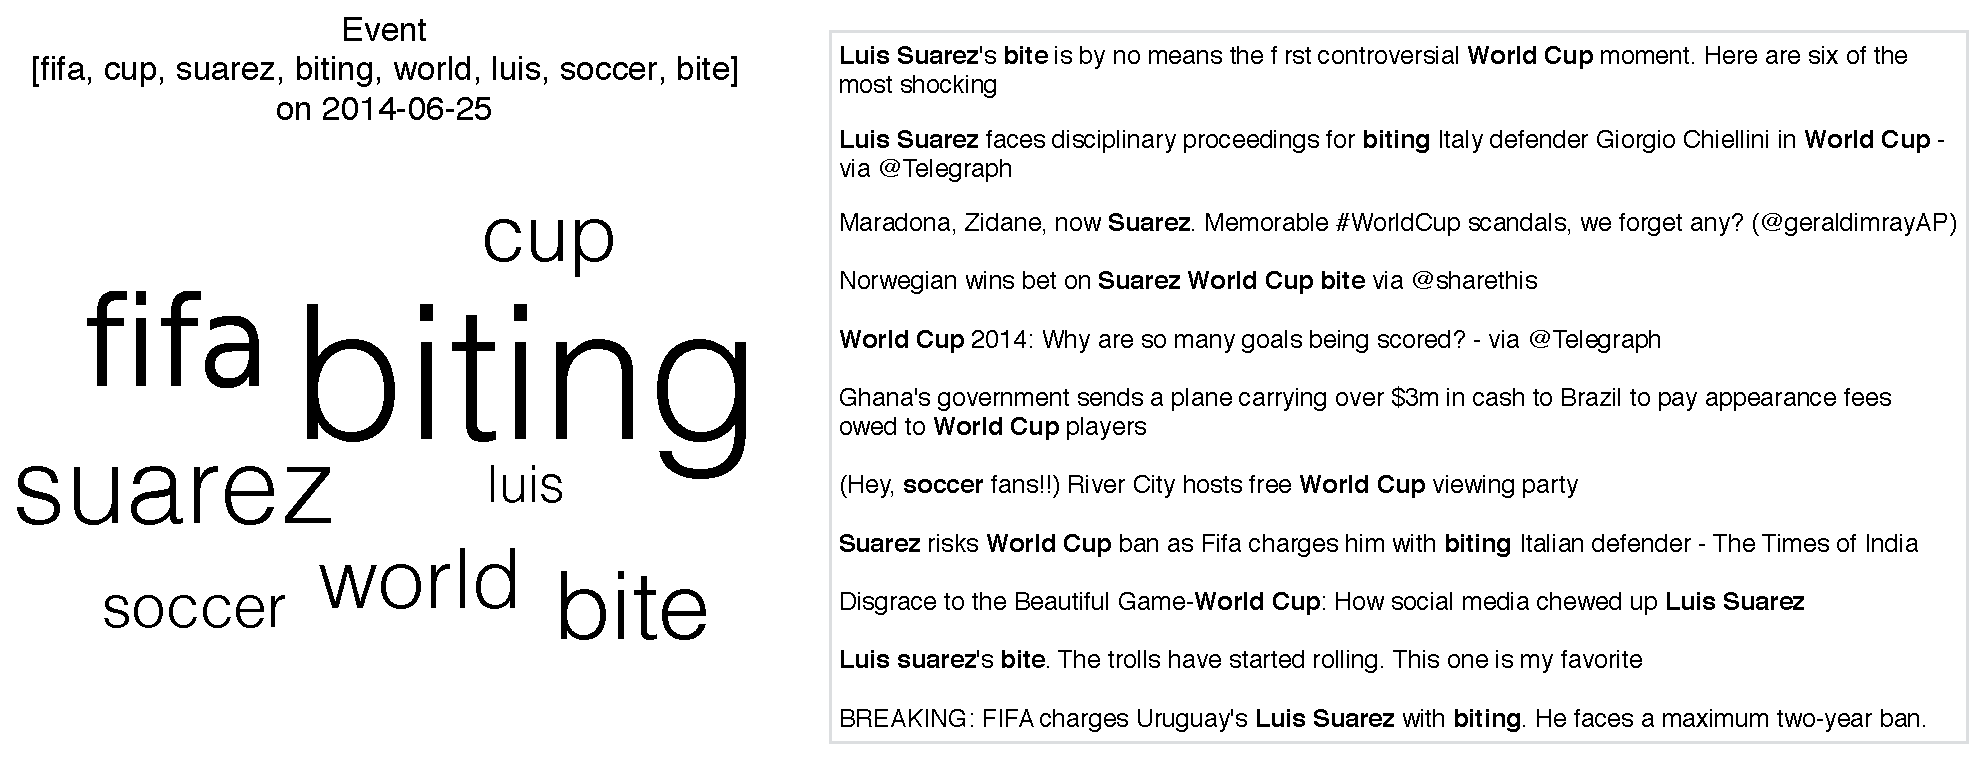
\includegraphics[width=\textwidth]{figures/high-activity/fig2}
  \caption[Example event]{A representative event, collected on 2014-06-25 with
      keywords (left) and sample user posts (right) collected from the Twitter
      Search API. Collected user posts contain at least one pair of keywords. }
  \label{fig:hi:components}
\end{figure}


The collection of events is converted into their VQ-event model representation. 
%
Using this model, we can identify events that have produced similar levels of
activity in the social network. 
%
In other words, events are considered to have similar activity if the
inter-arrival times between their social media posts are similarly distributed,
implying a very much alike collective reaction from users to the events within a
group. 
%
In order to identify groups of similar events, we cluster the event models. 
%
We sort the resulting groups of events from highest to lowest activity,
according to the concentration of social media posts in the bins that correspond
to short inter-arrival times. 
%
We consider the events that fall in the top cluster to be high-activity events
as most of their inter-arrival times are concentrated in the smallest interval of
the VQ-event model.
%
In our dataset, these correspond to roughly 8\% of the events. 
%
We consider the next clusters in the sorted ranking to form medium-high activity
events, and so on. 
%
Thus we end with four groups of events: high, medium-high, medium-low and low.
Figure~\ref{fig:hi:heatmap} shows a heatmap of the inter-arrival relative
frequency for each cluster. 
%
This classification of events based on activity intensity is independent of
event size. 


\begin{figure}
  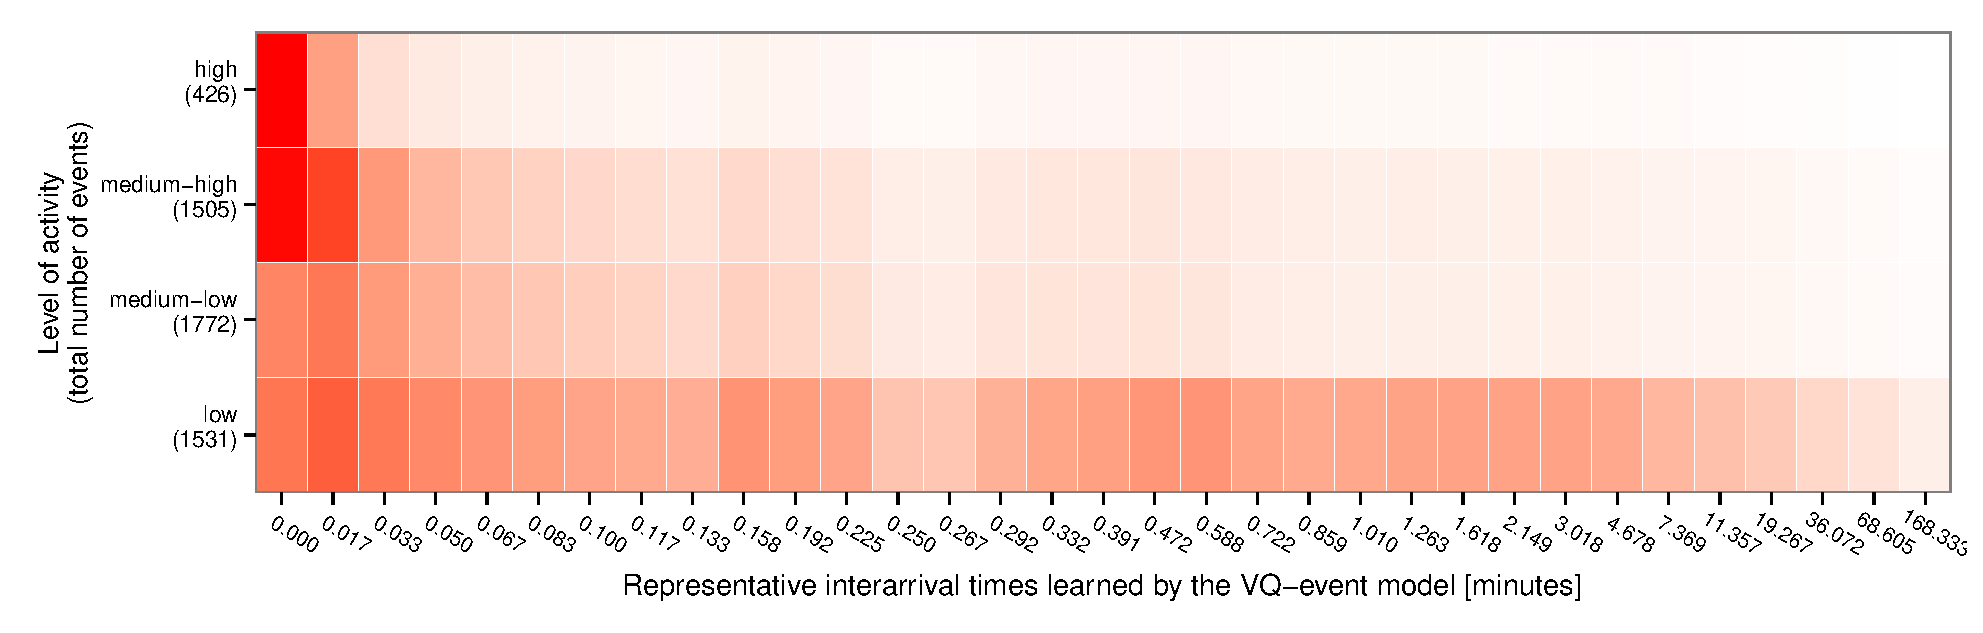
\includegraphics[width=\textwidth]{figures/high-activity/fig3}
  \caption[Heatmap of the categorization of events into clusters of
  activity.]{{Heatmap of the categorization of events into clusters of activity.
  Each row is the average representation of all the events in that clusters.  A
  darker cell represents a higher value. The y-axis specifies the number of
  events in that cluster. Clusters are (top to bottom): high-impact,
  medium-high, medium-low, and low.}}
  \label{fig:hi:heatmap}
\end{figure}
\section*{Results and Discussion}
%\newtext{ 
Our main objective in this work is to analyze the
  characteristics of high-impact events which differentiate them from
  other types of events. In particular, we identify how early in an
  event's evolution is it possible to determine if an event is going
  to be of high impact in the on-line social network.

Tables~\ref{table:high-impact-sample}
and~\ref{table:low-impact-sample} show examples of events from the high-impact category and 
low-impact category. We recall that the high-impact
events are those which were in the top 8\% of the ranking obtained by
sorting the event clusters according concentration of social media
posts in bins that correspond to the shortest time interval.  Table
\ref{table:high-impact-sample}, shows two events of different sizes
(large and small) and different scopes (one global and the other more local)
categorized as high impact in our dataset. The first event, the death
of Nelson Mandela, is one of the large events in the dataset, with
$\approx$ 134,000 tweets. The histogram representation of this event,
shown in Figure \ref{fig:nelson_mandela} suggested that more than $80\%$ of
the tweets arrived almost instantaneously. This is an event of
international political and social importance, which created an
overwhelming flood of messages on social media.  Hence, it makes sense
for such an example to be placed in the high-impact category.  The
second event, on the other hand, about the 2013 Mumbai Gang Rape is of
much smaller scale, with a total of $\approx$ 1,700 tweets.  However,
this event caused considerable amount of immediate reaction on social
media, with more than $48\%$ of its messages arriving almost
instantaneously.  Despite its smaller size, and its possible
confinement to a localized on-line community, this event has been
placed in the high-impact category.

Table \ref{table:low-impact-sample} shows events that have been
classified by our methodology in the category of low impact.  The
first event, about a teen surviving after hiding in the wheel of a
airplane, had only a little more than $25\%$ of its messages arriving
instantaneously although it had over 18,000 messages.  The second
event, about the damages caused by a tornado in Canada, did not garner
much immediacy in attention since only $7\%$ of its messages arrived
instantaneously. Most of the messages of this event were spaced out in
time. Even though, we cannot say whether or not this event had
significant implications in the real-world, we can say that it did not 
have considerable impact on the Twitter network. The lack of interest
could be due to several factors that are currently beyond the scope of
this work, ranging from the lack of Twitter users in the locality of
the event, to the fact that the tornado did not cause big damages. 

Fig.~\ref{fig:highest}, Fig.~\ref{fig:low}, Fig.~\ref{fig:cdf-highest} and
Fig.~\ref{fig:cdf-lowest} show the average histograms and the average
cumulative distribution functions of the events corresponding to the
high and low impact categories, respectively.  Visually, the average
high-impact event vector representations starkly differs from that of
a low-impact event in that the histogram in Fig.~\ref{fig:highest}
seems to possess an exponential decay, while the histogram in
Fig.~\ref{fig:low} does not.  To test this hypothesis, we fit
exponential function of the form $f(x)=ae^{bx}$ to the event
histograms. Table~\ref{tab:curve_fitting} summarizes the results from
statistical significance tests performed on the parameters $a$ and
$b$, and on the residual least squares error used for fitting the
exponential curves.  The differences between these values is
statistically significant ($p$-value $\leq2.2\times 10^{-16}$), thus demonstrating
that high-impact events, on an average, fit the exponential decay
curve much better than their low-impact counterparts.  In addition,
Fig.~\ref{fig:param_est} shows two scatter plots with the resulting
exponential parameters $a$ and $b$.  We observe that the majority
($97.4\%$) of high-impact events have an exponent $b \leq -50$,
separating them unequivocally from other events.
%}


 

\begin{figure}
  \centering 
  \begin{subfigure}{\textwidth}
    %\includegraphics[width=\textwidth]{figures/avg_hist_3_7}
    \caption{High-impact event summary histogram. %\inote{Mauricio:
                                %change label for the   x-axis}
    }
    \label{fig:highest}
  \end{subfigure}%

  ~%add desired spacing between images, e. g. ~, \quad, \qquad, \hfill etc.
  % (or a blank line to force the subfigure onto a new line)
  \begin{subfigure}{\textwidth}
    %\includegraphics[width=\textwidth]{figures/avg_hist_0_1}
    \caption{Low-impact event summary histogram. %\inote{Mauricio:
                                %change label for   x-axis}
    }
    \label{fig:low}
  \end{subfigure}%
  ~ %add desired spacing between images, e. g. ~, \quad, \qquad, \hfill etc.
  % (or a blank line to force the subfigure onto a new line)

  \caption{\textbf{Fig.~\ref{fig:highest} and~\ref{fig:low} show the average
    histogram of the high-impact and lowest impact groups respectively in our dataset. The $y$-axis is in square root
      scale.
      % \inote{change labels of x and y axis}
    }}\label{fig:histograms}
\end{figure}
\begin{figure}
  \centering
  \begin{subfigure}{.5\textwidth}
    %\includegraphics[width=\textwidth]{figures/cdf-highest}
    \caption{Average cumulative distribution function of high-impact events. %\inote{Mauricio:
                                %change label for the   x-axis}
    }
    \label{fig:cdf-highest}
  \end{subfigure}%
  ~%add desired spacing between images, e. g. ~, \quad, \qquad, \hfill etc.
  % (or a blank line to force the subfigure onto a new line)
  \begin{subfigure}{.5\textwidth}
    %\includegraphics[width=\textwidth]{figures/cdf-lowest}
    \caption{Average cumulative distribution function of low-impact events. %\inote{Mauricio:
                                %change label for   x-axis}
    }
    \label{fig:cdf-lowest}
  \end{subfigure}%
  ~ %add desired spacing between images, e. g. ~, \quad, \qquad, \hfill etc.
  % (or a blank line to force the subfigure onto a new line)

  \caption{\textbf
      % \inote{change labels of x and y axis}
    }}\label{fig:cdfs}
\end{figure}


\begin{figure}
  \centering
  \begin{subfigure}{.5\textwidth}
    %\includegraphics[width=\textwidth]{figures/param_est_a}
    \caption{Coefficient $a$ parameter estimation summary per event impact category. %\inote{Mauricio:
                                %change label for the   x-axis}
    }
    \label{fig:param-a}
  \end{subfigure}%
  ~%add desired spacing between images, e. g. ~, \quad, \qquad, \hfill etc.
  % (or a blank line to force the subfigure onto a new line)
  \begin{subfigure}{.5\textwidth}
    %\includegraphics[width=\textwidth]{figures/param_est_b}
    \caption{Exponent $b$ parameter estimation summary per event impact category. %\inote{Mauricio:
                                %change label for   x-axis}
    }
    \label{fig:param-b}
  \end{subfigure}%
  ~ %add desired spacing between images, e. g. ~, \quad, \qquad, \hfill etc.
  % (or a blank line to force the subfigure onto a new line)

  \caption{\textbf{Fig.~\ref{fig:param-a} and~\ref{fig:param-b} show the parameter value estimation for $f(x)=ae^{bx}$.}}
  \label{fig:param_est}
\end{figure}


\begin{table}
  \centering
  \begin{tabularx}{\textwidth}{cccc}
    \toprule
    \textbf{Parameter} & \textbf{Mean (high-impact)} & \textbf{Mean (low-impact)} & \textbf{$p$-value} \\ \midrule
    $a$ & $0.7129$ & $0.0822$ & $\leq2.2\times 10^{-16}$  \\ 
    $b$ & $87.1903$ & $3.8013$ &$\leq2.2\times 10^{-16}$ \\
    Error & $0.003$ & $0.008$ & $\leq2.2\times 10^{-16}$ \\ \bottomrule
  \end{tabularx}
  \caption{\textbf
    }}
  \label{tab:curve_fitting}
\end{table}

Further analysis of the high-impact events shows significant
differences to other events, in the following aspects: (i) how the
information about these events is propagated, (ii) the characteristics
of the conversations that they generate, and (iii) how focused users
are on the news topic. In detail, high-impact events have a higher
fraction of {\em retweets} (or shares) relative to their overall
message volume. On average, a tweet from a high-impact event is
retweeted 2.36 times more than a tweet from a low impact event. The
most retweeted message in high-impact events is retweeted 7 times more
than the most retweeted message in a medium or low impact event. We
find that a small set of initial social media posts are propagated
quickly and extensively through the network without any rephrasing by
the user (plain forwarding). Intuitively, this seems justified given
general topic urgency of high-impact events. Events that are not
high-impact did not exhibit these characteristics.

Our research also revealed that high-impact events tend to spark more conversation
between users, 33.4\% more than other events. This is reflected in the
number of {\em replies} to social media posts. The number of different
users that engage in high-impact events is 32.7\% higher than in
events that are not high-impact. Posts about high-impact events are
much more topic focused than in other events. The vocabulary of unique
words as well as {\em hashtags} used in high-impact events is much
more narrow than for other events. Medium and low impact events have
over 7 times more unique hashtags than high-impact events. This is
intuitive, given that if a news item is sensational, people will
seldom deviate from the main conversation topic.

% We have presented an analysis of high-impact news events based on
% the data of their entire life-cycle in the social network. We used
% the arrival time intervals to create a model that allows us to
% classify the event according to its impact. Nevertheless,

In a real-world scenario, in order to predict if an early breaking
news story will have a considerable impact in the social network, we
will not have enough data to create its impact-based model, i.e., we
will not yet know the distribution of the speed at which the social
media posts will arrive for the event. For instance, an event can
start slowly and later produce an explosive reaction, or start
explosively and decay quickly to an overall slower message arrival
rate. Still, reliable early prediction of very high-impact news is
important in many aspects, from decisions of mass media information
coverage, to natural disaster management, brand and political image
monitoring, and so on.

For the task of early prediction of high-impact events, we use features 
that are independent of our impact-based model, such as
the retweets, the sentiment of the posts about the event, etc. 
These features are computed on the early 5\% of messages about the event.
% More details are provided in the supplementary material.
The results are an average from a 5-fold cross validation with
randomly selected 60\% training, 20\% validation and 20\% test splits.
The high-impact events are identified with a precision of 82\% using
only the earliest 5\% of the data of each event
(Table~\ref{tab:classification_results}).  Additionally, we were able to
identify with high accuracy a considerable percentage of all
high-impact events ($\approx 46\%$) at an early stage, with very few
false positives (Table~\ref{tab:classification_results} and~\ref{tab:confusion_matrix}).

\begin{table}
  %\begin{adjustwidth}{-10mm}{-10mm}
  \centering
  {\small
    \begin{tabularx}{\textwidth}{lcccc|cccc}
      \toprule
      & \multicolumn{4}{c}{\textbf{Early 5\% Tweets}} & \multicolumn{4}{c}{\textbf{All Tweets}} \\
      \midrule
      & FP-Rate & Precision & Recall & ROC-area & FP-Rate & Precision & Recall & ROC-area \\
      % \midrule
      high-impact & 0.009 & 0.819 & 0.455 & 0.900 & 0.01 & 0.830 & 0.540 & 0.945 \\
      non-high-impact & 0.545 & 0.954 & 0.991 & 0.900 &  0.460 & 0.960 & 0.990 & 0.945 \\
      \bottomrule
    \end{tabularx}
  }
  \caption{\textbf{Classification of high-impact events.}}
  \label{tab:classification_results}
  %\end{adjustwidth}
%                                                                                                                                448,1         93%
\end{table}

\begin{table}
  \centering
  % {\scriptsize
  \begin{tabularx}{\textwidth}{lcc|cc}
    \toprule
    \multirow{2}{*}{ }& \multicolumn{2}{c}{\textbf{Early 5\% Tweets}} & \multicolumn{2}{c}{\textbf{All Tweets}} \\
    \midrule
    % \cmidrule{2-5} \cline{2-5}
    & high-impact & non-high-impact & high-impact & non-high-impact \\
    % \midrule
    high-impact & $194$ & $232$ & $230$ & $196$\\
    non-high-impact & $43$ & 4,765 & 47 & 4,761 \\
    \bottomrule
  \end{tabularx}
  % }
  \caption{\textbf{Confusion matrix for high-impact events prediction.}}
  \label{tab:confusion_matrix}
\end{table}



The precision using only the early tweets is almost as good as using
all tweets in the event (0.819 to 0.830). This suggests that the
social network somehow acts as a natural filter in separating out the
high-impact events fairly early on.  The recall goes from 0.455 to
0.540. This indicates that there are some high-impact events which
require more data in order to determine what kind of impact they will
produce, or events for which impact occurs due to random conditions. A
detailed description of the features and different classification
settings are provided in the supplementary material.%\supplementary.
\section{Chapter Summary and Conclusions}

In this chapter, we studied the characteristics of the activity that news events
produces in the Twitter social network. 
%
In particular, we proposed to measure the impact of the real-world news event on
the online social network by modeling the user activity related to the event
using the distribution of their inter-arrival times between consecutive
messages.
%
In our research we observed that the activity triggered by real-world news
events follows a similar pattern to that observed in other types of collective
reactions to events, 
%
namely by displaying periods of intense activity as well as long periods of
inactivity.
%
This model of user activity allowed us to perform high-level analysis of news
events, by characterizing them and identifying groups of similar user activity.


We extended this analysis by identifying groups of events that produce
a much greater concentration of high-activity than other events. 
%
We showed that there are several specific properties that distinguish how
high-activity events evolve in Twitter, when comparing them to other events. 
%
We designed a model for events, based on the code-book approach, that allows us to
do unambiguous classification of high-activity events based on the impact
displayed by the social network. 
%
This definition does not have some of the problems that current notions of
virality and popularity have. 
%


Some notable characteristics of high-activity events are that they are forwarded
more often by users, and generate a greater amount of conversation than other
events.
%
Social media posts from high-activity news events are much more focused on the
news topic. 
%


Our experiments showed that there are several properties that can suggest early on
if an event will have high-activity in the online community. 
%
We can predict a high number of high-activity events {\em before} the network
has shown any type of explosive reaction to them. 
%
Using simple off-the-shelf feature based classifiers, we can predict many
high-impact events with high precision. 
%
This suggests that users are collectively quick at deciding whether an event
should receive priority or not. 
%
However, there does exist a fraction of events which will create high activity,
despite not presenting patterns of other high activity events during their early
stages.
%
These events are likely to be affected by other factors, such as random
conditions found in the social network at the moment and require further
investigation.
\chapter{Spatio-Temporal Context: Inferring Geopolitical Interactions on Twitter}



\section{Introduction}\label{sec:geo-introduction}

The immense growth of the social Web, which has made a large amount of user data
easily and publicly available, has opened a whole new spectrum for research in
social behavioral sciences.  
%
However, as the volume of social media content increases at a very fast rate, it
becomes extremely difficult to systematically obtain high-level information from
this data.  
%
As a consequence, tasks related to the analysis of historical news events based
on social media data have not been explored, which limits any type of
comparative historical research, causality analysis, and discovery of knowledge
from patterns extracted from aggregated social media event information.

In this chapter we target this issue by proposing a compact high-level
representation of news events using social media information. 
%
This representation explicitly includes temporal information about the event and
information about locations, in particular of geopolitical entities. 
%
We call this a {\em spatio-temporal context-aware event representation}. 
%
Our hypothesis is that by including social, temporal, and spatial information in
the event representation, we are enabling the analysis of historical world news
from a social and geopolitical perspective.  
%
This facilitates, new information retrieval tasks related to historical event
information extraction and international relations analysis. 
%
We support our claims by presenting a quantitative analysis of a 2-year Twitter
dataset of news events reported by U.S. and U.K.  media, which we explore using
data mining techniques on our event representations. 
%
We also show how using a visual tool, named Galean, we can explore and retrieve
historical news events within their geopolitical and temporal context.



As social media becomes massively popular, it is increasingly being used as a news source.  
%
Many users turn to social media platforms to obtain information, especially
breaking news~\cite{Rogers:2013:DTT:2464464.2464511}. 
%
Even traditional mass media organizations such as newspapers and TV news
channels now use social media platforms to inform their audience more quickly.
%
Social media users are not only consumers of this information, but also
producers and broadcasters. 
%
Millions of people from all over the world have assumed the task of reporting
and commenting on newsworthy events.  
%
In particular, the social platform Twitter has become a preferred source for
users to find up-to-date information.  
%
When breaking news occurs, Twitter users quickly react by generating content and
producing interactions.  
%
The particular nature of Twitter messages, as well as the fact that most of its
users use the platform from mobile devices, facilitates extremely fast
information propagation.

%%% NEED - why something needed to be done at all
%
Twitter provides excellent conditions for social behavior analysis, as well as
comparative historical research, among many other social and scientific
disciplines.  
%
In particular, the field of {\em comparative historical
research}\footnote{\url{https://en.wikipedia.org/wiki/Comparative_historical_research}
(Accessed: June 19, 2019.) See also
\url{https://en.wikipedia.org/wiki/Comparative_research} (Accessed: June 19,
2019)} examines historical events in comparison to other historical events to
gain general knowledge that goes beyond a particular event. 
%
So far, historical research had been restricted to traditional archival data and
historians' written account of past events. 
%
Nevertheless, it is undeniable that the data poured into social media about
world events is of great value to society. 
%
The evidence is in the increasing body of scientific work surrounding retrospective
microblog data.  
%
Just to mention a few examples: Castillo et al.~\cite{castillo2011information}
extracted information to predict the credibility of rumors in social media,
Sakaki et al.~\cite{Sakaki2010} used Twitter for real-time earthquake detection,
Pak and Paroubek~\cite{Pak:Twitter:2010} studied Twitter messages as a corpus
for sentiment analysis, and Saravanou et al.~\cite{Saravanou:Twitter:2015} used
tweet coordinates to find locations that have been affected by floods.

%%

Despite the usefulness of historical information extracted from social media,
there is not much research addressing the topic of retrospective analysis of
this data.
%
Social media in general, and Twitter in particular, produce streaming data that
is volatile, which most likely explains why existing research concentrates only
on a particular event.

%%% Task - what the we undertook to address the need (first person, past
%%% tense)
We addressed this issue by introducing novel data mining tasks, based on a
compact representation of real-world news events. 
%
This representation was designed to summarize information about real-world
events from social media data, which is enhanced with the event's geographical
and temporal context.

%%

Our event representation incorporates two types of spatial data about an event:
%
1) locations directly {\em involved} in the real-world event occurrence (i.e.,
the main places that are mentioned in messages about the event), which we refer
to as {\em protagonist locations}, and 
%
2) locations from where social network users {\em comment} on the event (i.e,
the places where users that comment are located), which we refer to as {\em
interested locations}.  
%
For example, when an earthquake took place in Nepal in April, 2015, most of the
messages mentioned Nepal, which indicated that this was the location where the
event had taken place. 
%
Therefore, if we consider locations at a country level, Nepal can be regarded as
the {\em protagonist location} of that event. 
%
However, the users that posted the messages about Nepal were distributed all
over the world, indicating that this event had global impact. 
%
Furthermore, some countries had more users interested in the event than other
countries, such as, neighboring countries and countries with citizens among the
victims.  
%
These would be considered as the {\em interested locations} of that event.

%%

Our work is based on the hypothesis that by adding spatio-temporal context to
news events, such as protagonist and interested locations, and the time at which
it occurred, we can discover new information based solely on social media data.
%
In particular, the application of our event representation allows us to find
relationships among events and among locations, such as:

\begin{enumerate}
\item{\bf event similarity:}
  \begin{itemize}
  \item {\bf based on their protagonist locations}, i.e., retrieve all the
    events that occurred in certain location, or that directly involved similar
    groups of locations;
  \item {\bf based on the locations that are interested in the event}, i.e.,
    retrieve all of the events that produced the similar interest in other
    locations.
  \end{itemize}
\item{\bf location similarity:}
  \begin{itemize}
  \item {\bf based on events in which a location is protagonist}, i.e., retrieve
the locations that are protagonists in the same events;
  \item {\bf based on their interest in events}, i.e.,  retrieve sets of
locations that showed similar levels of interest in the same events.
  \end{itemize}
\item{\bf any combination of the above.}
\end{enumerate}

These similarity relationships along with temporal context can facilitate the
implementation of novel information retrieval tasks. 
%
These tasks include: event search, event understanding, geopolitical analysis,
international relations analysis (when considering locations at a country
level), historical comparative analysis, among others.

\paragraph{Contributions.} Our contributions are the following:

\begin{enumerate}
\item We present a novel high-level representation of news events based on
information extracted from social media. This representation emphasizes the
geographical and temporal context of news;
\item We present an exploratory analysis of a 2-year data collection in which we
use our proposed event representation to identify connections and similarity
patterns among countries; and
\item We show how a visual tool, named Galean, designed for exploration of
historical news event collections based on our proposed approach, allows users
to view event evolution over long periods of time, the relationship between the
geopolitical entities that participate in them, and emergent patterns.
\end{enumerate}

An application of the model and visual tool proposed in this chapter and
corresponding publications can be found in the work of Maldonado et
al.~\cite{maldonado2015spatio}.
%
They show a version of Galean specifically designed for exploring Chilean news.
%
An online version of this application can be found in \url{http://galean.cl/}
(Accessed: October 18, 2020).
\subsection{Background}\label{sec:related}

Certain studies focused specifically on the task of detecting events and tagging
their relevant geo-locations. 
%
In particular, some works targeted the detection of localized
events~\cite{Watanabe:Jasmine:2011,Abdelhaq:EvenTweet:2013,Walther:2013fb,Lee:A:2011,Krumm:2015},
others the detection of global events~\cite{sankaranarayanan:twitterstand:2009},
and the detection of critical
events~\cite{Sakaki:Tweet:2013,DeLongueville:2009}.  
%
Dong et al.~\cite{Dong2015}, specifically, considered that events had different
temporal and spatial scales and proposed a multi-scale event detection approach
for social media. 
%
This approach focuses on detecting and reporting events with geo-localization.
%
Our current approach differs from existing work, in that we create an aggregated
representation of the information about real-world events, producing a
high-level representation that includes the event's geographical context, which
is extracted from social media. 
%
In addition, we enrich the information about an event by using the locations of
the users that post information about it.

Wang et al.~\cite{Wang:LeadLine:2012} visualized topics based on the extraction
of geographical entities from tweet text. 
%
They did not use this information to establish the location of an event, but
rather for event exploration. 
%
SensePlace2~\cite{MacEachren:SensePlace2:2011} is a Visual Analytics tool that
allows users to explore a set of tweets and models them by showing two
geographical types of information: the locations from where users discussed the
topic and the locations being mentioned in tweets. 
%
However, unlike our work, this information was only used at single tweet level,
and not at event level.

In the domain of cyber-physical systems, {\em events} are viewed as conditions
of interest~\cite{st-model_2009} within a cyber-physical system, or as the
co-occurrence of two people in the same physical place~\cite{STEvent_2010}.
%
In general, events are modeled according to the state of the objects in the
system, considering attributes, time and location. 
%
The work presented by Tan et al.~\cite{st-model_2009} bears certain similarities
with our own, in the sense that they considered an event to encompasses multiple
information about a condition of interest in the system (in our case in the
online social network), including time and physical locations. 
%
In addition, the authors defined different kinds of temporal and geographical
scopes for their events, which are similar to our definition of {\em event
impact}. 
%
The main difference relies in that our approach aims to capture high-level
information of how a complex exogenous event, such as a news event, is perceived
by social network users in an aggregated way. 
%
Therefore, we focus on geopolitical divisions as units of aggregated spatial
information and on representing geopolitical interactions.

%%

Despite that the idea of adding spatio-temporal context to social media data is
not novel, to the best of our knowledge our work is the first that formally
introduces {\em protagonist} and {\em interested} locations in a high-level
event representation.  
%
The novelty of our approach relies on the extension of the notion of spatial
context, first by associating real-world news to one or more protagonist
locations, and second by associating real-world news to the locations where they
generated interest.  
%
In addition, our work does not focus on event detection, classification or
summarization, as most of the prior work on event analysis does.

\paragraph{Quantitative Historical Event Analysis.}
We provide a revision of the literature on {\em quantitative history} research
applied to event analysis and social media. Quantitative history is an approach
to historical research that makes use of quantitative and digital
tools. 
%
To the best of our knowledge, our work is among the first to make use of social
media data for quantitative historical research.

Prior work used digitized newspapers and books for extracting quantitative
knowledge~\cite{Michel176,leetaru2011culturomics,chadefaux2014early}. 
%
Michel et al.~\cite{Michel176} built a corpus of 5 million books and analyzed
them using word frequencies to investigate cultural trends, and called this type
of study ``Culturomics.''
%
Leetaru~\cite{leetaru2011culturomics} performed a large-scale study of 30 years
of digitized newspapers.
%
Chadefaux~\cite{chadefaux2014early} used a dataset from Google News Archive to
predict military conflicts.

A different line of research covers digitized writings and the Semantic Web.
%
Suchanek and Preda~\cite{Suchanek:2014:SC:2732977.2732994} proposed the study of
``Semantic Culturomics'', in which the analysis of newspapers should go beyond
the study of word frequencies in order to integrate knowledge bases (such as
DBPedia~\cite{dbpedia}) to answer complex user queries. 
%
Additional research has used knowledge bases along with human writings, such as
newspapers~\cite{Huet:2013:MHL:2509558.2509567,DS/CN175}. 
%
A survey on this topic is provided by Mero\~no-Pe\~nuela et
al.~\cite{merono2014semantic}.

Compared to prior work, our approach among the first to consider user-generated
information networks, such as online social networks, which are a growing data
source at much larger scale.  
%
We consider that social media can provide additional and novel information to
that found in news articles and books. 
%
User-generated content reflects social opinions and points of view related to
current world-events. 
%
This content is generated in real-time, it is not edited and does not depend on
the editorial lines of formal news outlets.  
%
We believe that these unique characteristics make social media a challenging and
valuable source of historical information.  
%
Our approach incorporates the content of social media platforms about real-world
news, as well as aggregated geographical information that conveys the importance
and scope of these events.
\section{Event Representation}\label{sec:geo:model}

We introduce a novel high-level event representation, called {\em
spatio-temporal context-aware event representation}, with the purpose of gaining
insight about real-world news from social media as well as from the relations
between locations and impact that these events induce. 
%
Specifically, we define our event representation and how it can be used to study
relations among locations.

\subsection{Event Representation Definition}\label{sec:model_definition}

We represent an event as a complex information unit that encompasses all of the
available social media content associated with a certain news topic, as well as
its aggregated spatial and geographical information.
%
%Events are represented
%as: i) the set of {\em keywords} that describe a particular news topic,
%and ii) the set of all of the {\em social media messages} that discuss the
%event, posted during the timeframe of its occurrence.
%
%We modify the aforementioned model by adding spatial and temporal context of
%the event's high-level abstraction.
%
In particular, we incorporate information about the locations involved in the
event occurrence, and the locations of the users that post messages about the
event. 
%
This representation is solely based on the social media activity surrounding the
event in the online social network, without including any external information
sources.
%
Specifically, we define two types of spatial contexts, which we call:
\begin{enumerate}
\item {\bf protagonist locations}, which are the locations involved in the
event, and
\item {\bf interested locations}, which are the locations from where users
comment on the event.
\end{enumerate}

For example, consider the news about Chile and Peru's maritime dispute at The
Hague in The Netherlands~\cite{bbc_peruchile}. 
%
If we define locations at country level, then this is an event for which Twitter
users mention mostly three countries when discussing the event: Chile, Peru and
The Netherlands (other mentions are negligible). 
%
Hence, according to our definition this event is considered to have three
protagonist locations. 
%
However, users that comment on this event are located mostly in: Chile, Peru,
Argentina and Bolivia. 
%
Therefore, the event is considered to have four interested locations.

More formally, we define an event $E$ as a tuple of the form:
%
\begin{equation} \label{eq:event}
E = (K, D, T, \mathbf{P}, \mathbf{I})
\end{equation}
%
%\medskip
\noindent where $K$ is  a set of keywords, which succinctly describe the news
topic, $D$ is the date of the event detection, $T$ is a set of tweets about the
event, published by users of online social networks.
% Tweets are also defined as tuples of the form
%$t = (u, l, m, d)$ for any tweet $t \in T$, where $u$ denotes the user who posted
%$t$, $l$ denotes the location of the user $u$, $m$ denotes the message text contained in $t$, and $d$
%denotes the date when $t$ was posted.
In addition, consider $L=\{l_1, l_2,\ldots, l_{|L|}\}$ to be the set of existing
locations. 
%
We augment the information about the event by explicitly including its spatial
context with the vectors $\mathbf{P}$ and $\mathbf{I}$, which correspond to the
{\em protagonist} and {\em interested} location values, respectively, for the
event $E$. 
%
This is, the $j$-th dimension of vector $\mathbf{P}$ contains the number of
times that the location $l_j$ is mentioned by the tweets in $T$. 
%
On the other hand, the $j$-th dimension of vector $\mathbf{I}$ contains the
number of tweets in $T$ that were posted by users in the location $l_j$.


Using the information introduced by vectors $\mathbf{P}$ and $\mathbf{I}$ we can
derive the scope of an event $E$ from two perspectives, {\em provenance} and
{\em impact}, defined as follows:
%\bp{See if these are the best names.. not sure yet}

\begin{itemize}
\item{\bf Provenance:} 
%
Indicates whether an event is local, regional or global in terms of the
locations it involves.
%
We consider an event to be of {\em local provenance} if it involves only one
protagonist location. 
%
We consider an event to be of {\em regional provenance} if it involves two or
more protagonist locations that are all from a same region (e.g., for countries,
this means neighboring countries or from a same continent\footnote{According to
the division that considers 7 continents: Asia, Africa, Europe, North America,
South America, Antarctica and Australia.}). 
%
We consider an event to be of {\em global provenance} if it involves two or more
protagonist locations in which at least one is not from the same region. 
%
Vector $\mathbf{P}$ contains this information for a given event $E$.


\item{\bf Impact:} 
%
Indicates if an event is local, regional or global in terms of how many
locations show interest in it. 
%
We consider an event to be of {\em local impact} if it generates conversation
from users in only one location (i.e., one interested location). 
%
We consider an event to be of {\em regional impact} if it generates conversation
from users in more than one interested location, all from the same region.  
%
We consider an event to be of {\em global impact} if it generates conversation
from users in more than one interested location in which at least one of those
locations is not from the same region. 
%
Vector $\mathbf{I}$ contains this information for a given event $E$.
\end{itemize}

For example, the message {\em ``Australia confirms signals detected by China
`consistent' w/ \#MH370 black box''}, discussed an event in which Australia and
China are involved. 
%
Therefore, Australia and China can be considered as protagonist locations in
this event. 
%
On the other hand, this particular news event was discussed extensively by users
located in several countries, including: USA, Canada, Colombia, U.K., India,
Nigeria, South Africa, Indonesia, Australia, France, Germany, China and Italy.
%
Therefore, this is an event that had {\em global provenance} (i.e., more than
one protagonist location from different regions) and {\em global impact} (i.e.,
more than one interested country from different regions).

%%

It should be noted that there can be different levels of ``global impact'',
depending on how many different locations show interest in the event (e.g., a
high-impact global world events will spark conversation in many countries). 
%
In addition, a location can be of any type of geopolitical division granularity,
such as a city, a region, a country, a continent, etc. 
%
However, for our work we focus on locations at {\em country level}. 
%
Therefore, at times we use the concepts of ``locations'' and ``countries''
interchangeably.
%
In particular, in the following section, we define a representation for
relations among locations, which we exploit in Section~\ref{sec:mining} for
extracting international relations.




\subsection{Representing Relations Among Locations}\label{sec:relations}

The spatio-temporal context-aware event representation allows us to extract
different types of relationships among locations for a given event collection.
%
In particular, we define a {\em protagonist-interest} vector $\mathbf{pi}$ for a
location $l_j$, which represents the interest that other locations have in
events that have $l_j$ as a protagonist.  
%
We define $\mathbf{pi}$ for $l_j$ as:

\begin{equation} \label{eq:pi}
%\mathbf{pi}(l_j) = \langle w(l_j,l_1),w(l_j,l_2),\ldots,w(l_j,l_{|L|}) \rangle
\mathbf{pi}(l_j) = \Big[ w(l_j,l_1),w(l_j,l_2),\ldots,w(l_j,l_{|L|}) \Big]
\end{equation}
%
\noindent where,
%
\begin{equation} \label{eq:pi-w}
w(l_j,l_k)=
f(\mathit{\#~of~events~that~have}~l_j~\mathit{as~protagonist}~\mathit{in~which}~l_k~\mathit{shows~interest}),~\forall~l_j,l_k \in L
\end{equation}
%
Likewise, we also define the {\em co-protagonist} vector $\mathbf{cp}$ for the
location $l_j$ as follows:
%
\begin{equation} \label{eq:cp}
%\mathbf{cp}(l_j) = \langle w'(l_j,l_1),w'(l_j,l_2),\ldots,w'(l_j,l_{|L|}) \rangle
\mathbf{cp}(l_j) = \Big[ w'(l_j,l_1),w'(l_j,l_2),\ldots,w'(l_j,l_{|L|}) \Big]
\end{equation}
%
\noindent where,

\begin{equation} \label{eq:cp-w}
w'(l_j,l_k)=
f(\mathit{\#~of~events}~l_j~\mathit{as~protagonist}~\mathit{in~which}~l_k~\mathit{is~also~a~protagonist}),~\forall~l_j,l_k \in L
\end{equation}

The relationships between locations, given by $\mathbf{pi}$ and $\mathbf{cp}$,
allows us to identify similarity relationships among locations, such as:

\begin{itemize}
\item{\bf Locations that produce similar interest:} 
%
from $\mathbf{pi}$ we can extract sets of locations (countries) that are
similar, based on the level of interest that they produce in other locations
(countries). 
%
For example, they can be obtained using $k$ nearest neighbors or by clustering
locations' $\mathbf{pi}$ vectors.

\item{\bf Locations that are protagonists of the same events:} 
%
from $\mathbf{cp}$ we can identify which locations (countries) are similar,
based on their interactions (i.e., they are protagonists of the same event) with
other locations (countries). 
%
For example, they can be obtained using $k$ nearest neighbors or by clustering
locations' $\mathbf{cp}$ vectors.
\end{itemize}

The weights, $w(l_j,l_k)$ and $w'(l_j,l_k)$, are expressed as a function
$f(x_{j,k})$, where $x_{j,k}$ corresponds to {\em \# of events in which $l_j$
and $l_k$ interact}. 
%
In particular, for Galean, users have expressed the preference of visualizing
the {\em absolute} number of events in which two countries interact (i.e.,
$f(x_{j,k})=x_{j,k}$).  
%
Nevertheless, there are other cases in which the analyst could prefer the
weights to reflect the fraction of events in which two countries interact in
relation to the total of events for one of the two locations (e.g., where the
number of events is normalized by the amount of events in which $l_j$ or $l_k$
participates).
%
This can be useful in cases that the number of events in which different
locations participate are very concentrated on specific locations. 
%
We explore cases such as these in Section~\ref{sec:mining}, where we analyze the
dataset which is biased towards certain countries.

%%

We note that weights can also be expressed as functions of the {\em \# of
tweets} or the {\em \# of users}, and in addition, the proposed representation
allows us to also specify {\em interest-interest} and {\em interest-protagonist}
vectors, in a similar fashion to $\mathbf{pi}$ and $\mathbf{cp}$. 
%
However, we do not focus on these variations in this dissertation.

\begin{figure}[h]
  \centering
  \includegraphics[width=\textwidth]{figures/geopolitical/k_accuracy_recall.pdf}
  \caption[Mean and standard deviation of multi-label scores]{Mean and standard
  deviation of multi-label scores of accuracy, precision, recall and F1 measure
  by $\alpha$ ratio for 100 randomly selected events from our dataset.}
  \label{fig:eval}
\end{figure}

\medskip
\paragraph{Precision and recall of event locations.}
%
Empirically, we observed that the precision and recall of the locations
considered to be protagonist of an event depends mostly on a ratio, which we
call $\alpha$.
%
For an event $E$ that contained more than one location, we defined $\alpha$ as
the minimum percentage of tweets that must refer to a location $l_i$ in relation
to the most mentioned location $l_{\mathrm{max}}$, in order for $l_i$ to be
included in $\mathbf{P}$ or $\mathbf{I}$ vectors.
%
Figure~\ref{fig:eval} shows an empirical analysis of the effect of $\alpha$ on
the precision, recall and $F_1$ metrics of protagonist locations on a sample of
100 events.  
%
Precision and recall were estimated based on a manual assessment of the
protagonist locations of those events. 
%
Based on this variation $\alpha$ can be set as the value that provides the best
tradeoff between $F_1$ and recall ($\alpha = 19\%$ in our experiment).

In addition, if $E$ has only one location $l$, we require that this location is
mentioned a minimum percentage of tweets, which we define as $\beta$. This ratio
is also defined within the same experimental scenario, determined from the
smallest percentage of mentions that $l$ can have in relation to the total
number of tweets in $E$, for a given $\alpha$.



\subsection{System Architecture}\label{sec:framework}

We present a general overview of the architecture for generating our event
representations in order to use them in our application.  
%
The architecture, shown in Figure~\ref{fig:sys_architecture}, consists of the
following three parts: {\em ``input''}, {\em ``event representation
generator''}, and {\em ``visualization''}.  
%
The first component, (1) ``input'', is not part of the particular contribution
of this chapter\footnote{The {\it News event extractor} module is part of our
data collection methodology, as described in Chapter~\ref{chapter:data}}, and is
currently fulfilled by using existing methods, which can be replaced
transparently as long as the requirements detailed next are met. 
%
On the other hand, the other two components, (2) ``event representation
generator'' and (3) ``visualization'', are the core of our contribution and
therefore essential to our system.


\begin{figure*}[t]
    \includegraphics[width=\textwidth]{figures/geopolitical/architecture.pdf}
    \caption[Data architecture for Spatio-Temporal Model.]
    {Framework consisting of three parts: 1) input, which collects data related
    to news event activity from social media and extracts its geographical
    information; 2) the event representation generator, which generates our
    representation of the input events and 3) the visualization, which consumes
    these events. Our contribution is related to the two latter modules, the
    first module can be replaced according to the task and/or state-of-the-art.}
    \label{fig:sys_architecture}
\end{figure*}

Given an input from the Twitter data stream we specify the following components
of our framework:

%%

\begin{enumerate}

\item{\bf Input:} 
%
This module requires two subparts, the {\em ``news event extractor''} and the
{\em ``geographical context extractor''}.
%
    \begin{enumerate}
    %
    \item{\em News event extractor:} 
    %
    This submodule must output groups of tweets, where each group of tweets $T$
    should represent a cohesive news topic $E$.  
    %
    In particular, most of the tweets in the set $T$ of an event $E$ must be on
    the topic of a particular news events. 
    %
    However, as we use a high-level representation of events, some noise is
    tolerated (i.e., tweets that do not correspond to the event).

    \item{\em Geographical context extractor:} 
    %
    This submodule associates spatial context to each tweet in $T$ of each event
    $E$ produced by the ``news event extractor'' module. 
    %
    Therefore, it must provide the geographical locations of the places
    mentioned in the text of the message and the geographical location of the
    author of the message (i.e., protagonist and interested locations,
    respectively). 
    %
    This module must locate the majority of the tweets in $E$ correctly (i.e.,
    with good precision) based on GPS coordinates and/or textual content, so
    that locations mentioned in tweets can be geotagged, and users can be
    geotagged as well (users can set their location using GPS coordinates or by
    using natural text).

    \end{enumerate}
%
\item{\bf Event representation generator}: 
%
This component creates the event representations $E$ for each of the groups of
tweets provided by the ``input'' module. 
%
In particular this module is responsible for creating a tuple $E$ for each
event, as specified by our definition in Section~\ref{sec:model_definition}.
%
This means that it has to produce the date $D$ of the first tweet, a set of
keywords $K$ that describe the event, the set $T$ of tweets and the $\mathbf{P}$
and $\mathbf{I}$ location vectors of the event.

%%

\item{\bf Visualization}: 
%
This module consumes the event representations
produced by the ``event representation generator'' module and produces the event
visualization interface.

\end{enumerate}



\noindent{\bf News event extraction setup.} 
%
The news event extraction module corresponds to that proposed in
Chapter~\ref{chapter:data}, which consists of an ongoing process that
periodically retrieves tweets about real-world news. 
%
The process produces coherent sets of tweets about news topics, although with
certain degree of noise that is well tolerated by our system. 
%
In particular, this is a two-stage iterative process that consists of the
following steps:
%
(1) {\em news topic identification} (i.e., detection), and 
%
(2) {\em event tweet extraction}. 


\smallskip
\noindent{\bf Geographical context extraction setup.}
%
We create a methodology for extracting the protagonist and interested locations,
as well as their frequency for an event $E$ with a set of tweets $T$.  
%
The {\em toponym} (i.e., location name) extraction and resolution phases are
carried out using the off-the-shelf geoparser, CLAVIN~\cite{clavin}. 
%
However, since tweets are short and do not provide much context for toponym
disambiguation, our methodology boosts the performance of the geoparser by
adding context from other tweets in $E$.

As detailed in Section~\ref{sec:geo:model}, this methodology relies in a ratio
named $\alpha$ which we empirically set to $19\%$ as that which provides the
best tradeoff between F1 and recall, according to Figure~\ref{fig:eval}. 
%
This is, a location must have at least $19\%$ of the mentions of the most
frequent location of an event, to be considered as part of that event as well.
%
Otherwise, we consider that this location was not actually involved in the
event.


\noindent{\bf Dataset Description.} 
%
The data used in this work corresponds to events from August 2013 to June 2015.
%
This dataset consisted of 20,066 news events, which contained 193,445,734 tweets
produced by 26,127,624 different users.

We note that our event representation and applications are independent of the
data extraction methodology.  
%
Therefore, in order to improve the representativeness of our event collection in
the future, less biased methods of event extraction can be used, such as
automatic event detection techniques~\cite{Metzler_2012, Choi_2012} and/or the
integration of more comprehensive sets of seed news sources, as done for Chilean
news analysis by Maldonado et al.~\cite{maldonado2015spatio}.


\section{Exploratory Analysis}\label{sec:geo:mining}
% Implementation

We present an exploratory data mining analysis that uses the information
provided by our spatio-temporal context-aware event representation.  
%
We describe our empirical findings, which illustrate the usefulness of our
proposed event representation.  
%
This analysis considers the location context of events at the country-level
geopolitical division.  
%
This allows us to explore the international interactions given by our current
dataset. 


The event extraction process, described in Chapter~\ref{chapter:data}, was based
on a seed set of internationally renowned news media accounts that publish
information in English. 
%
This introduced a certain bias in our event collection towards events that took
place in English speaking countries, and towards including more tweets in
English than in other languages. 
%
For example, for the event {\it ``correspondents dinner''} our current method
will mostly retrieve tweets in English from users world-wide. 
%
On the other hand, an event described with a set of keywords which includes {\it
``Barack Obama''} will retrieve tweets in several languages. 

%%

These biases must be taken into consideration because they can limit the
representativeness of the findings yielded by our data mining analysis.
%
Nevertheless, we believe that they do not invalidate our results, which show the
perspective of a subset of the social network that is centered on news reported
in the United States and Great Britain. 
%
Therefore, our results reflect the world-view of these two overly represented
countries in particular, and of English-speaking users in general.
%
Furthermore, other studies using the full Twitter stream, such as that of
Poblete et al.~\cite{Poblete:2011:BTS:2063576.2063724}, show a similar data
distribution to ours, indicating that this type of bias could be inherent to
Twitter itself.

%%

Furthermore, an in-depth exploration of the bias in our dataset showed that the
number of tweets produced during an event did not depend on the number of seed
accounts that covered that event. 
%
Our analysis showed that only $13.5\%$ of the users in the entire collection had
actually reposted a tweet from the seed news media accounts, which gives the
overall impression that these accounts did not influence much the amount of
interest expressed by users. 
%
Also, we found no relation between the number seed accounts that shared an event
and the number of countries that participated in the event in terms of
provenance or of impact. 
%
(There was no Pearson correlation between the proportion of different news
outlets and the number of different users, the protagonist countries, or the
number of tweets from each interested country.)

%%

As mentioned in Section~\ref{sec:relations} we used a normalization for vectors
$\mathbf{pi}$ and $\mathbf{cp}$, defined in Equations~\ref{eq:pi}, \ref{eq:pi-w}
and \ref{eq:cp}, \ref{eq:cp-w}, respectively. 
%
This normalization allows us to compare protagonist-interest and co-protagonist
vectors in a way that mitigates the bias of overrepresented countries. 
%
In particular, for the $\mathbf{pi}$ vector we defined $w(l_j,l_k)$ as:

$$w(l_j, l_k) = f(x_{j,k})= \frac{x_{j,k} - \mu(\mathbf{x}_{\cdot,k})}{\sigma(\mathbf{x}_{\cdot,k})}$$

\noindent and for $\mathbf{cp}$ we defined $w'(l_j,l_k)$ as:

$$w'(l_j, l_k) = f(x'_{j,k})= \frac{x'_{j,k}}{x'_{j}},$$

\noindent where $x_{j,k}$ was the number of events that have $l_j$ as
protagonist in which $l_k$ is interested; $\mathbf{x}_{\cdot,k}$ is the vector
containing the number of events in which location $l_k$ is interested, $\forall
l_j \in L$; $\mu$ and $\sigma$ are the mean and standard deviation of the
distribution of events, respectively; $x'_{j,k}$ is the number of events for
which both $l_j$ and $l_k$ were protagonists, and $x'_{j}$ is the number of
events that had $l_j$ as protagonist.

% These normalizations
%are optional and not part of our model, as they are not always used by
%the application, such as the case of our visualization tool presented
%in Section~\ref{sec:vis}.
\begin{figure*}[t]
\centering
\includegraphics[width=\textwidth]{figures/geopolitical/choropleths.pdf}
\caption{Summary maps of interest and protagonists.}\label{fig:maps}
\end{figure*}

\begin{figure*}[t]
\centering
\makebox[\textwidth][c]{\includegraphics[width=1.1\textwidth]{figures/geopolitical/coprot.pdf}}%
%\includegraphics[width=1.1\textwidth]{figures/geopolitical/coprot.pdf}
\caption{Relative co-protagonist measure of selected countries.}\label{fig:coprotagonism-ind}
\end{figure*}

% tweets & users per country
\begin{figure*}[t]
\centering
\makebox[\textwidth][c]{\includegraphics[width=1.15\textwidth]{figures/geopolitical/tweets-users.pdf}}%
%\includegraphics[width=1.1\textwidth]{figures/geopolitical/tweets-users.pdf}
\caption{Description of the bias in the number of tweets and users, per country.}\label{fig:tweets-per}
\end{figure*}



We started by characterizing the spatial distribution of our collection to
describe its representativeness in terms of geographical coverage. 
%
In terms of protagonist locations, the United States and Great Britain were the
protagonists of the majority of the events, followed by India, Australia,
Ukraine and Russia (Figure~\ref{fig:maps} (a)). 
%
The median number of events in which countries were protagonist is $18.5$,
indicating that only a few countries were the protagonists of the majority of
events. 
%
Figure~\ref{fig:maps} (a) shows the distribution of the number of events in
which countries were protagonists. 
%
When we computed the $\mathbf{cp}(c_i)$ vectors for selected $c_i$ countries
(Equation~\ref{eq:cp}, normalized by the number of events in which a country
$c_i$ is protagonist), we observed that the United States and Great Britain were
the protagonists of the majority of international events
(Figure~\ref{fig:coprotagonism-ind}). 
%
There are some exceptions, such as Ukraine, which had only Russia as the
co-protagonist many of its international events
(Figure~\ref{fig:coprotagonism-ind} (d)).
%There are some exceptions, such as Ukraine which co-protagonizes most of its events
%with Russia (Figure~\ref{fig:co-prot-ua}).

%%

In terms of worldwide interest, the countries that displayed interest in most
events were the United States, Great Britain and India (Figure~\ref{fig:maps}
(b)).  
%
In addition, these countries also contributed the most tweets
(Figure~\ref{fig:tweets-per} (a)).

We determined the location for 37.3\% of the users (9,738,538 out of 26,127,625
users). 
%
These users were mostly distributed among the United States and Great Britain,
followed by Canada, Indonesia and India (Figure~\ref{fig:tweets-per} (b)).
%% \bp{should
%% we say that it is reasonable to expect the geolocated users to be
%% sampled randomly among locations?}

\medskip
\noindent{\bf International relations exploration.}
We explored the dataset in order to identify similarity between countries
according to the events in which they are co-protagonists and the interest shown
towards these events by the rest of the countries in the world. 
%
We found that applying standard similarity metrics over the data in the event
representations, yielded relationships between certain countries that resemble
intense historical interactions and/or geographical proximity.

%\noindent \textbf{Country co-protagonism.}
In terms of protagonist locations, we found countries that were {\em similar},
meaning that they were protagonists of the same events. 
%
In this case we used the Jaccard similarity between each pair of countries as
our similarity measure, representing each country by the set of events in which
it was a protagonist. 
%
The Jaccard similarity between two sets $x$ and $y$ is defined as $sim_{x, y} =
\frac{|x \cap y|}{|x \cup y|}$.
%
We filtered out the countries that were protagonists of less than $130$ events
(corresponding to the 80-th percentile of events for which countries were
protagonist). \\

%
\paragraph{Significance of the Jaccard metric.}
%
We studied the distribution of our similarity metric, in order to determine
which relationships between countries were significant. 
%
We fitted the \emph{similarity} to a theoretical probability distribution using
the R package {\em
fitdistrplus}~\footnote{\url{https://CRAN.R-project.org/package=fitdistrplus}}
and we found that the best fit was a Gamma distribution with parameters
$shape=0.8721$ and $rate=85.7683$.
%
Based on this analysis, if $S$ is a random variable with a Gamma distribution
representing the similarities between countries, then we defined the similarity
between two countries $x$ and $y$ as being {\em significant} if its value was in
the 95-th percentile of the distribution, (i.e., if $P( S < sim_{x,y} ) >
0.95$).
%
Using this criteria, we determined a similarity threshold of $sim^*=0.032$,
above which we considered its value to be significant. 
%
This threshold can be parameterized at the 80-th, 90-th, or 99-th percentile, as
the researcher finds appropriate.  
%
Table \ref{tab:jacc} shows the top-20 most similar countries based on this
similarity, making it to the 97.181 percentile of our dataset. \\

\begin{table}
  \centering
  \footnotesize
\begin{tabular}{llrrrr}
\toprule
Country $i$ & Country $j$ & $x'_i$ & $x'_j$ & Similarity & Percentile\\
\midrule
Israel & Palestine & 561 & 360 & 0.2863 & 99.969\\
Russia & Ukraine & 823 & 921 & 0.2094 & 99.906\\
North Korea & South Korea & 158 & 179 & 0.1866 & 99.843 \\
Great Britain & United States & 4,015 & 10,162 & 0.0966 & 99.248\\
Iraq & Syria & 654 & 647 & 0.0833 & 99.092\\
\addlinespace
India & Pakistan & 1,561 & 453 & 0.0753 & 98.998\\
Iran & Israel & 496 & 561 & 0.0698 & 98.841\\
China & Japan & 646 & 354 & 0.0605 & 98.340\\
France & Germany & 627 & 371 & 0.0583 & 98.184\\
\addlinespace
Argentina & Brazil & 130 & 236 & 0.0578 & 98.152\\
Australia & Great Britain & 974 & 4,015 & 0.0577 & 98.090\\
Brazil & Germany & 236 & 371 & 0.0575 & 98.058\\
Syria & Turkey & 647 & 198 & 0.0536 & 97.964\\
\addlinespace
Iran & Iraq & 496 & 654 & 0.0512 & 97.777\\
Australia & Malaysia & 974 & 262 & 0.0492 & 97.682\\
Argentina & Germany & 130 & 371 & 0.0481 & 97.620\\
Australia & India & 974 & 1,561 & 0.0475 & 97.495\\
\addlinespace
Germany & Greece & 371 & 155 & 0.0457 & 97.401\\
Canada & Great Britain & 715 & 4,015 & 0.0444 & 97.275\\
Egypt & Libya & 316 & 253 & 0.0440 & 97.213\\
Great Britain & India & 4,015 & 1,561 & 0.0436 & 97.181\\
\bottomrule
\end{tabular}
\caption[Most similar countries in terms if co-protagonism]{Most similar
countries in terms of being protagonists of the same events
(\emph{\textbf{co-protagonist}} vector), using Jaccard Similarity. $x'_i$ is the
number of events in which country $i$ was a protagonist.}\label{tab:jacc}
\end{table}

\begin{table}
  \footnotesize
  \centering
\begin{tabular}{llrrr}
\toprule
Country $i$ & Country $j$ & $x'_i$ & $x'_j$ & Distance\\
\midrule
Turkey & Indonesia & 198 & 172 & 1.1442\\
Yemen & Turkey & 202 & 198 & 1.3416\\
Afghanistan & Turkey & 323 & 198 & 1.5304\\
Libya & Turkey & 253 & 198 & 1.6050\\
\addlinespace
Egypt & Palestine & 316 & 360 & 1.6496\\
Malaysia & Turkey & 262 & 198 & 1.8096\\
Japan & Spain & 354 & 258 & 1.8327\\
Italy & Japan & 315 & 354 & 1.9018\\
\addlinespace
Brazil & Spain & 236 & 258 & 1.9060\\
Germany & Pakistan & 371 & 453 & 2.0674\\
Israel & Syria & 561 & 647 & 2.4463\\
Russia & Ukraine & 823 & 921 & 2.5557\\
\addlinespace
Nigeria & Pakistan & 412 & 453 & 2.5822\\
Canada & China & 715 & 646 & 2.6025\\
Iran & Syria & 496 & 647 & 2.6838\\
Iraq & Iran & 654 & 496 & 2.9270\\
\addlinespace
France & Canada & 627 & 715 & 3.7859\\
Australia & France & 974 & 627 & 4.1398\\
India & Australia & 1,561 & 974 & 4.8339\\
Great Britain & India & 4,015 & 1,561 & 41.7719\\
\bottomrule
\end{tabular}
\caption[Similar countries in terms of participation vectors]{Pairs of countries
that had the closest $\mathbf{pi}$ vectors according to the Euclidean Distance.
$x'_i$ is the number of events in which country $i$ was a
protagonist.}\label{tab:euc}
\end{table}


% prot
We found that Israel and Palestine were the most similar countries, followed by
Russia and Ukraine, North Korea and South Korea, Great Britain and the United
States, and Iraq and Syria (Table~\ref{tab:jacc}). 
%
Their similarities are higher than the 99.25\% of the pair-wise similarities in
our dataset.
%
There are real-world historical and geographical relations between those
countries that can account for these similarities (for example, the Ukrainian
crisis~\cite{ukranian_crisis}, or the Israeli-Palestinian
conflict~\cite{israeli_palestinian}). 
%
On the other hand, some of the similarities can be explained by the
preponderance of certain events, such as the 2014 FIFA World Cup.
%(Table~\ref{tab:jacc-knn}).
These results indicate that there is information in Twitter data about
real-world geo-political interactions which can be further studied using our
event representation.

\begin{figure}
    \centering
    \makebox[\textwidth][c]{\includegraphics[width=1.15\textwidth]{figures/geopolitical/graphs.pdf}}%
    \caption[Graphs of similar countries]{Similarity graphs of countries using
    the Jaccard similarity as the weight for the edges. Each node is a country
    and an edge between two nodes corresponds to the Jaccard similarity between
    those two countries. An edge is present if the similarity is higher than the
    given threshold. The node size and color represents the number of events in
    which each country was a protagonist, and the thickness of and edge
    represents the similarity.}\label{fig:sim-graph}
\end{figure}

In Figure~\ref{fig:sim-graph}, we present three graphs where countries represent
nodes and edges are weighted based on the Jaccard similarity. 
%
As we increase the threshold to connect two countries with an edge, communities
of countries emerge. For example, in Figure~\ref{fig:sim-graph} (c), it is
possible to identify a group consisting of Germany, Mexico, Brazil, Argentina,
Netherlands, Spain and Italy: countries whose teams participated in the 2014
FIFA World Cup. 
%
It is also possible to observe edges among Malaysia, Indonesia, China and
Australia, reflecting the disappearance of the Malaysia Airlines flight MH370 on
2014. 
%
Those two long-term events, for instance, sparked several events in our dataset,
and the interactions between the protagonist countries are reflected in our
analysis.

\begin{figure}
    \centering
    \includegraphics[width=\textwidth]{figures/geopolitical/jaccard_time.pdf}
    \caption[Timeseries of the Jaccard similarity between co-protagonist
  vectors]{Timeseries of the Jaccard similarity between co-protagonist vectors
  of selected pairs of countries over time. The value of similarity is computed
  for all the events in the given week. Data from October 2014 and December 2014
  was not available.}\label{fig:time-series}
\end{figure}

\paragraph{Time series co-protagonism.}
We further explored trends of co-protagonism by analyzing the similarity of
countries over time. 
%
Given two countries, we computed their Jaccard similarity based on the events of
a time window of one week. 
%
Figure~\ref{fig:time-series} shows the time series between United States and
Great Britain, Malaysia and Australia, and Russia and Ukraine. 
%
Each of those pairs of countries showed different characteristics in terms of
how their similarity evolved over time. 
%
The US and Great Britain did not show notorious bursts of similarity over time,
although they had high overall Jaccard similarity (Table~\ref{tab:jacc}),
showing that although they were co-protagonists in several events, there was not
a particular situation that suddenly increased their similarity in a narrow time
span. 
%
On the other hand, Malaysia and Australia showed a burst starting in March 2014,
shortly after the disappearance of the Malaysia Airlines flight MH370 (similar
patterns arose when inspecting the relationship with Indonesia and China).
%
Finally, Russia and Ukraine showed high values of similarity over time, starting
roughly in December 2013 and those patterns were maintained throughout 2014.\\


% interest

Another aspect that we explored was the interest that different countries had in
events that occured in different geographical regions. 
%
In other words, we explored the \emph{protagonist-interest} relationship between
countries. 
%
To do this, we represented each country $c_i$ as its corresponding
$\mathbf{pi}(c_i)$ vector (Equation~\ref{eq:pi}).


\begin{figure*}[t]
\centering
\includegraphics[width=\textwidth]{figures/geopolitical/int_prot.pdf}
\caption[Protagonist-interest plots for selected
countries.]{Protagonist-interest plots for selected countries.  Each plot shows
the level of interest ($y$-axis) displayed by the other counties of the world
(listed along the $x$-axis) in the events of the featured pair of ``protagonist
countries''. Country labels in the $x$-axis have been omitted for readability
purposes.}
\label{fig:int-prot}
\end{figure*}

We adjusted the original representation of the protagonist-interest vectors
(Equation~\ref{eq:pi}) in order to mitigate the data bias, which was reflected
in that some countries were overly represented, because they produced much more
tweets than others (Figure~\ref{fig:tweets-per} (a)). 
%
Then, instead of counting the number of events with $c_j$ as a protagonist, for
which $c_i$ expressed interest, we preferred to measure the interest of $c_i$ in
$c_j$ as the difference between the average number of events of other countries
in which $c_i$ was interested, with respect to the number of events of $c_j$ in
which $c_i$ was interested. 
%
In other words, our original interest measure was normalized by the average
interest shown by $c_i$ in other countries. 
%
Using this new interest measure we applied Euclidean distance to find the
country $c_2$ with the closest $\mathbf{pi}$ vector to another country $c_1$
(Table~\ref{tab:euc}).
%
Given that there were countries that expressed interest in only a few events, or
that were protagonists themselves of very few events, we only report the
countries that were protagonists of at least 167 events (i.e., the average
number protagonist events per country in our dataset).

%%

We observed that Turkey had strong ties with other countries, being very close
with several other countries according to protagonist-interest relations, such
as Indonesia, Yemen, Afghanistan, Libya, and Malaysia. 
%
Furthermore, other similar countries were Italy and Japan, Brazil and Spain (and
also Brazil and Germany); these similarities are be explained by the events
triggered in the 2014 FIFA World Cup.
%
Notably, Russia and Ukraine standout again, showing not only that they were
protagonists of roughly the same events, but also that they were seen with
similar interest by the rest of the world, making the impact that the Ukrainian
crisis had on the news more evident.
%
We also noted that most of these countries are close geographically, and as well
as other countries, mostly from Asia.
%
We argue that these results are another sign of the bias in our dataset: the
perspective of international news as seen by English-speaking countries.

\begin{table}[t]
\centering
{\footnotesize
\begin{tabularx}{\textwidth}{@{}lrrrr@{}}
\toprule
Event Description & Tweets & Users & Outlets & Countries\\
\midrule
Death of actor Robin Williams (2014) & 1.8M & 1.3M & 48 & 202\\
FIFA World Cup final between Germany and Argentina (2014)  & 494K & 385K & 40 & 144\\
FIFA World Cup starts (2014)  & 476K & 358K & 45 &  143\\
Super Bowl starts (2015)  & 1.1M & 849K & 35 & 130\\
New Year's Eve (2013)  & 325K & 279K & 31 & 127\\
Soccer Player Luis Suarez is suspended from World Cup (2014)  & 213K & 157K & 38 & 106\\
Charlie Hebdo shooting in Paris (2015)  & 629K & 328K & 50 & 102\\
Grammy Awards (2015)  & 682K & 432K & 31 & 97\\
Boxing match between Mayweather and Pacquiao (2015)  & 779K & 522K & 37 & 97\\
\bottomrule
\end{tabularx}
}
\caption[Events with most international impact]{Events with most international impact, measured as the number of countries which showed interest higher than the 99-th percentile of overall interest.}\label{tab:impact}
\end{table}


% Please add the following required packages to your document preamble:
% \usepackage{booktabs}
\begin{table}
\centering
{\footnotesize
\begin{tabularx}{\textwidth}{@{}lrrr@{}}
\toprule
Event Description                                                 & Tweets & Distinct Users & Outlets \\ \midrule
US Supreme Court ruled in favor of same-sex marriage              & 51K  & 50K          & 7                                    \\
Delhi Legislative Assembly election                               & 35K  & 13K          & 3                                  \\
Labour party said it will scrap the non-domiciled tax status      & 32K  & 15K          & 10                           \\
Tornado strikes Texas                                             & 31K  & 6K           & 4                                    \\
TV appearance of Delhi chief minister candidate Arvind Kejriwal   & 30K  & 10K          & 1                                    \\
Hillary Clinton announces presidential bid                        & 30K  & 30K          & 3                                     \\
Football player Cardale Jones announces he is returning to school & 28K  & 22K          & 3                                      \\ \bottomrule
\end{tabularx}
}
\caption[Events with most local impact]{Events with most local impact, measured as the number of tweets coming from events with only one interested country, whose interest is higher than the 99-th percentile of overall interest. All events happened on 2015.}\label{tab:impact_local}
\end{table}



Finally, we explored events with the highest impact, considering international
and local events.  
%
For this analysis, we considered all international events (regional and global).
%
We counted the number of different interested locations for each event, however
only considering interest measurements within the 99-th percentile of the
dataset.
%
From this analysis we were able to observe that the events with the highest
overall impact covered several topics, and that the most recurrent events were
sports and entertainment.  
%
Events like the death of the actor Robin Williams caused the most international
impact, with a large number of tweets from 202 countries.  
%
This was followed by sports events, such as the 2014 FIFA World Cup, the 2013
Super Bowl and the boxing match between Floyd Mayweather and Manny Pacquiao
(Table~\ref{tab:impact}).
%
Other events with high impact included New Year's Eve for 2013, the
\emph{Charlie Hebdo} shooting in Paris, and the Grammy Awards in 2015.  
%
We also observed that the coverage of different news outlets was higher for
these events.
%
On the other hand, events with local impact consisted mostly of political
events, such as political elections and debates, with the exception of a natural
disaster and a sports event.
%
We observed that in this case the coverage of different news sources was lower
in relation to high impact international events, as well as the number of tweets
involved.

%%

The source code of the analysis above and more examples can be found in the
following URL: \url{https://users.dcc.uchile.cl/~mquezada/galean/analysis.html}
(Accessed: June 21, 2019).
\section{Known Limitations}\label{sec:limitations}
\todo[inline]{poner esto en las conclusiones o en el chap3}
There are several limitations that we consider important to address. 
%
In particular, these limitations are not related to our proposed event
representation, framework and implementation of our applications, but rather to
the data extraction methodology which depends on external functionalities.

The news event extraction methodology relies on the headlines published by news
media accounts. 
%
This technique provides good precision in terms of reporting events that did in
fact exist in the real-world, but might omit informative events that did not
receive media coverage.
%
Therefore, the current data extraction approach can fail to retrieve events such
as citizen movements and other important events that were informed only via
social networks.  
%
In addition, in the current data extraction setup the initial seeds for the
event collection came from a reduced list of news media accounts, with limited
country coverage and languages.
%
Although the news event dataset likely represents a great majority of the news
events and related tweets posted on Twitter, the collection will miss the long
tail of events that had impact in other less represented countries worldwide. 
%
We note that there are several ways in which this bias can be mitigated in the
future, all of them related to replacing external modules in the data input
phase of the framework.

In addition, we note that although our proposed event representation can be
considered generalizable to other social media platforms, we have not validated
it on other sources of information besides Twitter. 
%
It is not certain that for other social media platforms we will have enough
information, regarding user location and data availability, in order to produce
accurate event representations.

Overall, basic future improvements of our work should consider:
%
\begin{itemize}
\item Implementing automatic event detection techniques for Twitter based on the
data stream and network properties, as well as more comprehensive microblog
event extraction approaches.

\item Improving the geolocation tool accuracy. Despite CLAVIN's maturity as a
geolocation tool, it does not recognize location names in languages other than
English (even though the documentation of the tool indicates that it does
recognize alternative location names~\cite{clavin}).

\item Adding finer granularity to the geographical context extractor of our
system, in order to include more precise administrative divisions such as cities
and states.

\item Merging events that discuss the same news topic in different languages.
Recent approaches in cross-language microblogging retrieval
\cite{Godavarthy2016} can be integrated for news event retrieval within our
framework.
\end{itemize}

All of these improvements are however beyond the current scope of our work,
which focuses on providing proof of the usefulness of the proposed event
representation. 
%
Nevertheless, we are working on improving all of these features in future
versions of our applications.  
%
For example, we have already started the task of providing more fine-grained
locations for Chile and comprehensive sets of local news sources as in the work
of Maldonado et al.~\cite{maldonado2015spatio}.



\section{Conclusions and Future Work} \label{sec:conclusions}


We have presented a spatio-temporal context-aware representation for news events
in social media. 
%
Using this representation we have introduced a visual analytics tool named
Galean that allows for retrospective analysis of real-world events through the
aggregation of information posted by social media users. 
%
The main goal of our tool and our event representation is to allow exploration
and quantitative analysis of events from a geographical and temporal
perspective. 
%
In particular we introduce two types of geographical contexts for events: 1)
protagonist locations, and 2) interested locations. 
%
The first corresponds to locations, in this case geopolitical divisions, that
were involved in the event itself, and the second corresponds to locations where
the event's information had the most impact.


In addition, we introduce a quantitative data mining study over a 2-year Twitter
dataset, in which we explore the properties of news events in social media and
the international relations that are induced by those events.  
%
Our findings indicate that indeed there is new information, which can be
extracted at large scale, about how countries relate and how information is
perceived in different places. 
%
Most interestingly, these relationships reflect historical relations that are
found in the real world, indicating that there is value in social media data for
historical research.
%
Overall, our representation allows us to perform new IR tasks, related to
exploring international relations and historical event retrieval.

\todo[inline]{future work aca o al final?}

In the future we will extend our representation to incorporate higher-level
temporal properties of events, such as if the event is long-term, punctual or
recurring, as defined in the work of Tan et al.~\cite{st-model_2009}.
%

Another interesting line of research for future work is that of studying how
pairwise similarities between countries evolve over time. 
%
This could be useful to automatically discover when new relationships arise and
when deviations from normal patterns occur.

Finally, we are researching techniques to improve data extraction for news
events, based on techniques such as those reported by Hasan et
al.~\cite{doi:10.1177/0165551517698564}, to achieve a better representation of
different locations, and to improve geolocation. 
%
We are also working towards creating automatic summaries of events in social
media, on how to track and visualize event evolution over time. 
%
In particular the relations among protagonist countries that happen as
consequence of these events, as well as incorporating approaches of
cross-language information retrieval\cite{grefenstette2012cross} for news event
recommendations in microblogs.
\chapter{Aggregating Content: A Lightweight Model of News Events}
\label{chapter:url}

\section{Introduction}
\label{sec:introduction}

%\mq{hablar de multimodal summarization, diferentes tamaños de topicos, clustering incremental, 
%redundancia ayuda a word embeddings?, complejidad de otros metodos}

%%%%% Index
% Context
% Motivation
% Problem statement
% Contributions

%%%% Content


% Context 
% \subsection{context}

%Un modelo de "representacion" de informacion (de evento en SM) de manera compacta 
%para incorporar nuevo conocimiento.... con aplicaciones A, B y C

%Una forma de modelar la informacion .... (alto nivel)
%Describir semi-formalmente el modelo 
%Poder separar "señales" o "aspectos" del evento 

%Presentar casos de estudio que muestren las N aplicaciones. Mostrar ejemplos de 
%cada aplicacion.

%ej, aplicacion "event retrieval": dado un evento, identificar contenido relevante, topicos o aspectos
%relevantes al evento real (?) 

%modelo con WE exacerba diferencias en los documentos para separar topicos usando UCG (redundancia)

%hipotesis con respecto a agrupar por url: contenido relevante es mas probable de ser compartido con las mismas
%urls que contenido no relevante 


% Nowadays, social media platforms have become a main source of news. According to
% a recent survey, by 2018 about two thirds of US adults used social media as a
% source of news~\cite{pewresearch}, and about 70 percent of Twitter users get
% news from there. With their scale, popularity, and ease of use, social media
% platforms have drastically lowered the entry barriers to disseminate newsworthy
% information in real time. 
%Due to that, news events are often reported earlier in
%social media than in traditional news media. 

% In particular, impactful or breaking real world events (such as the 2015 Nepal
% Earthquake or the 2017 Brexit) overflow social media with millions of messages.
% For that reason, it is a hard task for humans to go through every message in
% order to understand what an event is about. 


The sheer amount of newsworthy information published by users in social media
platforms makes it necessary to have efficient and effective methods to filter
and organize content. 
%
In this scenario, off-the-shelf methods fail to process large amounts of data,
which is usually approached by adding more computational resources. 
%
Simple data aggregations can help to cope with space and time constraints,
while at the same time improve the effectiveness of certain applications, such
as topic detection or summarization. 


%
We propose a lightweight representation of newsworthy social media data. 
%
The proposed representation leverages microblog features, such as redundancy
and re-sharing capabilities, by using surrogate texts from shared URLs and word embeddings.
%
Our representation allows us to achieve comparable clustering results to 
those obtained by using the complete data, while reducing running time and 
required memory.
%
This is useful when dealing with noisy and raw user-generated social media data.


The overload of information in social media streams makes it difficult for users
to obtain a comprehensive account of different emerging events reported by
users.
%
%to get a complete picture of an event or find relevant messages.
%
The ability to identify and summarize relevant information about newsworthy
topics that are accounted for by users in social media can be of great use to
society.
%
This is particularly true in the case of high impact and breaking news, like
natural disasters and crisis situations~\cite{ICWSM1817816}.
%\bp{agregar mas citas}.
%
In general, social media platforms present their content to the consumer in one
of two ways: (1) by displaying user posts in reverse chronological order, or (2)
by displaying posts in a personalized fashion, showing first what they deem more
interesting to the user.
%
However, if the user 
%consuming social media content 
is seeking information about a specific event, the aforementioned approaches can
result also in unnecessary exposure to redundant, irrelevant, or even misleading
information.
%
In this context, delivery of key pieces of information to the user is important,
and even critical in some cases; 
%
for instance, social media is often used as a complementary source of
information for disaster management and
response~\cite{ICWSM1817816,Sarmiento:2018:DDE:3201064.3201077}
%\bp{agregar citas}
and also to obtain information about newsworthy events not yet reported by
formal news outlets. 
%
%In this sense, thThis need to produce high-quality real-time information requires effective ways to filter and organize information about real-world events on social media.
%

Despite the usefulness of social media as a worldwide news information source,
its consumption is not without challenges.
%
These challenges include, among many others, correctly assessing information
veracity and relevance to a specific topic, as well as dealing with a huge
volume of data with variable quality. 
%
%In this sense, the consumption of social media content for information seeking about particular events requires effective ways to filter and organize streaming data.
%%
%
%Specifically, the task of organizing and filtering
%
%Filtering and organizing information in social media can be a
%particularly challenging task.
%
In particular, we study Twitter, in which users can post text-based messages.
%
These messages, called {\em tweets} can include links to images, videos, to
external web-pages or to other tweets, making this platform's content multimodal.

%
%From the perspective of understanding current events, tweets contain a large volume of irrelevant and redundant content, which can often be misspelled, or unreliably capitalized, 
%
%On the other hand, we observe several 
The URLs shared in Twitter often link to varied types of media (articles,
images, or videos), which have been found useful for identifying conversation
topics~\cite{mishne2012twanchor}.
%
In the context of news events, users tend to quickly re-share information if the
event sparks high interest (see Section~\ref{subsec:info_forwarding}), which
results in many (near-)duplicate messages.
%
Dealing with content of these characteristics requires different approaches
than with traditional media~\cite{Alonso:2017:WHH:3091478.3091484}.
%
Prior work has acknowledged the need of techniques for dealing with this type of
social media data.



%%


In this work we focus on the problem of producing summarized representations of
social media data related to news events without significant loss of
information.
%
We present a compact representation for social media content related to news
events.
%
This representation allows us to preserve information about the topics involved
in an event, and to identify relevant content, while reducing the volume of
data.
%
This can be especially useful for online data processing about developing news
and news information seeking tasks.
%
To achieve this, our model annotates shared URLs with the text of the messages
in which they appear.
%
Here we use messages as {\em anchor text} or {\em surrogate text}. 
%
We first leverage this idea by identifying relevant URLs that are shared in
social media during a news event.
%
We discard URLs that are too general with respect to an event (e.g. a general
report), or generic (e.g. linking to the homepage of a news outlet) as we deemed
them as non-relevant.
%
Then we aggregate all the anchor texts associated with relevant URLs into {\em
documents}, and all the conversations around those documents as well. 

As a preliminary way to study the usefulness of our event representation, we
applied it to three news events as a case study.
%
We observed that our representation reduces the amount of records needed to
describe an event by one order of magnitude, compared to using the raw tweets. 
%
We were also able to identify sub-topics by clustering the documents using dense
word representations, such as neural network--based word embeddings. 
%
We show that the clustering based sub-topic detection task using our proposed
representation yields similar external quality metrics to those obtained using
the entire data. 
%
Hence, indicating that we are preserving relevant aspects of the information
while considerably reducing running time.

\paragraph{Contributions.} Our contributions in this chapter are the following:

\begin{enumerate}
  \item We present a novel compact representation for news event information in
  microblogs, based on shared URLs. This representation reduces data volume.

  \item We study the usefulness of our representation through three case
  studies. We do so by introducing a methodology to represent news events in
  Twitter and find sub-topics. We show that our approach displays comparable
  performance to baseline methods at a fraction of the computational resources.
\end{enumerate}


% problemas con representar social media content
% Representing content generally involves representing its constituent terms in
% another space. For instance, using weighted term frequency vectors, graph
% models, or probabilistic models over the distribution of terms. In social media,
% these methods result in highly dimensional sparse features, which are difficult
% to manage without large quantities of well-curated messages. On the other hand,
% it is not trivial to manage large scale data. Current methods can manage large
% volumes of messages at great computational expense or by splitting the dataset
% in smaller sets and dealing with them separately. For example, traditional ways
% of representation of text, such as term frequency weighting, involves the
% generation of thousands of dimensions on messages that are about 10 to 20 words
% long.

% Nonetheless, in the context of news events, user-generated content can be leveraged
% to estimate the relevance of the information and to annotate content from
% external sources. We start from the assumption that users share and comment on
% content that is relevant or interesting to them. Hence, the existence of several
% messages on a topic suggests that the topic is important to users. We can
% leverage this idea even futher: we can annotate the shared URLs in user posts
% with the same text that users put in the posts that contains those URLs. In the
% literature, the text that accompanies a URL is usually known as {\em anchor text}, or
%   {\em surrogate text}, and this idea has been extensively used in query log
% mining~\cite{Beeferman:2000:ACS:347090.347176,10.1007/978-3-540-30192-9_58}. We
% can also take advantage of the redundancy of posts in social media. When exposed
% to an emergent news, users tend to share information as quickly as
% possible~\cite{kalyanam2016prediction}, and this often results in duplicate and
% near-duplicate data. This information can be useful to assess the
% importance of certain aspects of the event. In this work, we exploit these clues
% in order to design a model to represent newsworthy information.

% reescribir
% We propose a lightweight representation of news events in Twitter by aggregating
% tweets based on the existence of shared URLs. Our representation groups tweets
% by common shared URLs into {\it components}, and also ignoring highly common
% URLs in the dataset, in order to avoid having large components of unrelated
% tweets. This representation reduces the amount of records to be processed by one
% order of magnitude, and we validate its capabilities by performing clustering on
% three selected news events to identify sub-topics. By using dense
% representations of words, such as neural network based word embeddings, our
% model generates a compact representation of news events. We show that we achieve
% similar performance on sub-topic detection at a fraction of the time and memory
% required. Our proposed representation allows us to process raw, un-curated
% Twitter data faster than with using individual tweets, and it is flexible enough
% to incorporate new data as the event evolves in time.

% We propose a simple model to represent information about news events in Twitter
% using aggregations of tweets that mention the same URLs, and that retweet or
% reply themselves. Then, we model the resulting sets of documents using dense
% vector representation of terms, such as neural word embeddings, using a corpus
% of 193 million news-related tweets. With this representation, we exploit
% features often discarded in similar works, such as repeated messages and URLs
% mentioned in tweets. This results in a smaller and more flexible representation,
% which allows us to perform some tasks more efficiently, and to incorporate new
% information to the model with little effort. Our event representation is
% compatible with current approaches regarding Twitter event data, such as event
% detection, filtering, and summarization. We show the effectiveness of this
% representation by characterizing topics in news events shared in Twitter, which
% can contain several repeated or irrelevant posts. The topics consist of diverse
% tweets that share URLs, which can be seen as a multimedia representation of
% topics, regardless of the content of these URLs (images, videos, news articles,
% etc.). 




% problemas: mucha info, redundante, etc. 
% explotamos eso para mejorar la origanizacion de la info
% mostramos que es util para: ...
% tiene estas caracteristicas: ...


% One particular problem is what is called information overload: when users are
% exposed to way more information than they can process and understand, and
% effective methods to find relevant information are missing, assuming that
% users know what they are looking for. In this context, automatic summarization
% was proposed as a way to tackle this problem. Given a document or a set of
% documents about a specific topic, the output of the summarization method is a
% gist that summarizes the content, under certain criteria and restrictions. 


% In this work, we approach the issue of information overload by modeling
% content associated with online news, as propagated on Twitter. 
% When a {\em breaking news} occur, users tend to share and
% forward information about it as quickly as possible {\bf REF PLOS}, and ...

% motivation
% \subsection{motivation} 
% user contributed content reflect opinions of users, not media
% importance given by users
% free annotations of urls 




% problems with social media
% \subsection{challenges}
% events are noisy (different levels of relevance)


% However, the scale and rate of publication makes it difficult to understand
% what is happening or what an event is about. Also, the presence of irrelevant
% posts makes it even more difficult to understand a specific event. Usually,
% when a user wants to know about a certain ocurrence, he or she performs a
% search using some keywords, and a chronologically ordered timeline of the most
% recent posts is then shown. In other cases, a special sorting is made in order
% to show the most relevant posts that specific user might like the most, or
% just the posts with the highest scores in terms of popularity. However, this
% is not enough to understand the different aspects or topics related to an
% event.

% Different approaches have been proposed to help users understand the content.
% For example, automatic text summarization is used in order to select the most
% salient phrases from a set of documents, aiming for optimizing diverse criteria,
% such as relevance, coverage, or popularity. However, nowadays online news media
% has increasingly shifted their focus towards multimedia content {insertar
% cita}. There have been some efforts in order to summarize content of different
% modalities, such as images or videos in isolation, but few consider a mixture of
% them. Our hypothesis is that a summary in different content modalities, such as
% images, videos, and text, is more effective than a text-only, or images-only
% summary in order to understand an event. In other words, our hypothesis is that
% a multimodal summary is more informative than a unimodal one. In this work, we
% discuss the challenges of the current approaches and tackle the problem of
% multimedia summarization of events in social media, by considering content
% independently of its nature.



% problem statement
% \subsection{problem statement}

% hypotheses
% \subsection{hypotheses}
% Hypotheses: 
% 1. grouping tweets by url improve the ...
% 2. the use of word embeddings (fasttext) improve the ...

% % contributions
% % \subsection{contributions}
% Our contributions are the following:
% \begin{enumerate}
%   \item We investigate 
%   \item
%   \item ?
% \end{enumerate}


% % outline of paper
% % \subsection{outline}
% This paper is organized as follows. Section ...

% % -----------------------------------------------------------------------

% % Twitter desc
% On Twitter, each post, called {\em tweet}, is a short text ---traditionally
% 140 characters long, but by the year of 2017 this limit was extended to 280
% characters---, which can contain arbitrary URLs, as well as {\em hashtags}
% (words prepended with a \#, serving to the tweet as tags), {\em cashtags}
% (prepended by a \$, serving as identifiers for stocks and shares), and mentions
% (names of Twitter users).

\subsection{Background}\label{sec:related}
% There is extensive work on automatic summarization on microblogs\mq{ref}. In
% this work, we approach the problem from a practical point of view, where our
% goal is to benefit from the characteristics of social media posts, in
% particular, from event-related messages. We exploit the redundancy of
% information available in social media via the aggregation of information
% around shared URLs, and propose a simple and compact model using word
% embeddings on tweets. Therefore, we can classify the related work in three
% areas: modeling social media content, automatic summarization of news, and
% usage of word embeddings in social media.

Two lines of research are relevant to our work: the utility of anchor texts in
microblogs and topic detection methods using different aggregation strategies. 

%\bp{No hay literatura de representaciones compactas de eventos para sumarizacion?}

%
About the usefulness of anchor texts on Twitter, Raux et
al.~\cite{raux2011describing} used anchor texts from tweets pointing to a
predefined set of URLs to characterize general topics, by clustering a bipartite
graph of words and URLs. 
%
We instead focus on news events, and tweets related to these news, which have
their own particularities, in contrast to long lasting general topics. 
%
Mishne and Lin~\cite{mishne2012twanchor} studied the contribution of anchor
texts compared to the text of the websites behind the URLs, concluding that
anchor text add new terms not seen in the website content, by looking also at
the conversations around the sharing tweets. 
%
Alonso et al.~\cite{Alonso:2015:WCW:2740908.2745397} had similar findings
examining Facebook posts. 
%
In another work by Alonso et al.~\cite{Alonso:2017:WHH:3091478.3091484}, the
authors designed a social search engine using the propagation of shared URLs as
cues to measure virality, and anchor texts to augment metadata of the search
results with social content. 
%
In a previous work~\cite{quezada2013understanding}, we showed a proof of concept
of automatic summarization of documents using anchor texts.
%


Topic modeling of tweets is an active line of research, and there are some
studies which investigate the effectiveness of aggregation of tweets to improve
topic
detection~\cite{Hong:2010:EST:1964858.1964870,Mehrotra:2013:ILT:2484028.2484166,alvarez2016topic}.
Hong and Davison~\cite{Hong:2010:EST:1964858.1964870} analyzed the effects of
different aggregation strategies of tweets when finding topics with Latent
Dirichlet Allocation (LDA). 
%
They found that some schemes yield better results at some tasks, such as
classification problems related to tweets. 
%
In a similar fashion, Mehrotra et al.~\cite{Mehrotra:2013:ILT:2484028.2484166}
observed that aggregating hashtags (also described as {\em pooling} of tweets by
hashtags) is a more effective strategy to identify topics from tweets, but at
the cost of longer running times due to the duplication of tweets. 
%
Finally, Alvarez-Melis and Saveski~\cite{alvarez2016topic} found that adding the
threads of conversation into the pooling is more effective than pooling by
hashtag in their observations. 
%
We instead aggregate by shared URLs and conversations, with the goal of
generating a compact representation without major loss of information.



% \subsection{Using common information in tweets}

% Similar to our work, in the sense of exploiting common information across
% messages, the work of Kamath et al.~\cite{Kamath:2013:SDO:2488388.2488447}
% focuses in the spatio-temporal dynamics of {\em memes}, as seen as units of
% information spreaded in social media. For this, they model each tweet as a
% tuple of the hashtags involved, time, and location to observe and characterize
% topics in Twitter. Similarly, the work of Pe\~na-Araya et
% al.~\cite{pena2017gaining} aim to characterize geopolitical entities (such as
% countries) based on the tweets that mention them, by proposing a model to
% represent locations in a spatio-temporal ambit, and develop a visual analytics
% tool to explore events based on the location scope of their impact. Our work
% is similar to both in the sense of leveraging common entities across messages,
% in this case, the URLs, in order to generate a compact representation to
% facilitate the discovering of sub-events. In our case, we do so by using URLs
% and the text content as a surrogate for the URLs, also called anchor texts.

% Concerning the specific use of anchor text in social media, Mishne and
% Lin~\cite{mishne2012twanchor} show that the anchor texts in general tweets
% provide additional new information compared to the content of webpages alone
% in a study of 7 million URLs obtained from the Twitter Firehose. The work of
% Raux et al.~\cite{raux2011describing} is one of the first to use anchor texts
% to find clusters of topics in Twitter, in order to describe Web content using
% tweets. The authors create a weighted bipartite graph of tweet words and URLs,
% being the weight the tf-idf score of the words in the tweets that contain the
% URL, and then find clusters of URLs. Although they characterize clusters of
% URLs as topics, their work focuses on general tweets and not newsworthy
% messages in particular. In the work of Alonso et
% al.~\cite{Alonso:2017:WHH:3091478.3091484}, the authors develop a search
% engine for content related to URLs shared on Twitter, displaying the most
% popular and viral URLs, also showing the effectiveness of this approach. In
% our previous work~\cite{quezada2013understanding}, we show a prototype of a
% automatic summarization methodology using tweets aggregated by URL, and then
% modeling the aggregated sets as tf-idf vectors to cluster them, find sub-events, 
% and then selecting the most representative messages as a multi-modal
% summary.

% % \subsection{General text representation methods}

% % % verificar
% % %In a general domain, LDA is very good to find/extract topics, but not in the 
% % %domain of this work. So my magnificent research is pretty very much fabulous.

% % Topic models are a useful way to deal with textual information and to derive a
% % low-dimensional representation of documents. One of the most popular methods
% % is Latent Dirichlet Allocation, or LDA~\cite{blei2003latent}. LDA models a
% % document as a mixture of different topics, which are probability distributions
% % on the vocabulary. TwitterLDA~\cite{zhao2011comparing} is a modification to the 
% % original approach, by changing the assumption that a single document can discuss different topics, which may be unlikely in short messages, such as tweets. Our representation is 
% % compatible with LDA or TwitterLDA, as it provides a way to aggregate topical information which can
% % be used as input for topic models.

% % We also use dense word embeddings such as the continuous representations obtained by using shallow
% % neural networks such as {\tt word2vec}~\cite{DBLP:journals/corr/abs-1301-3781} 
% % or {\tt fastText}~\cite{bojanowski2016enriching}. Dense vector representation of words
% % provide a efficient way to assess the similarity of terms or documents. In contrast,
% % traditional methods, such as tf-idf~\cite{Salton:1983:EBI:182.358466}, involve generating embedding of words of thousands of dimensions, as high as the vocabulary size. Some methods, such as
% % Latent Semantic Analysis~\cite{dumais2004latent}, aims to reduce the dimensionality of the representation by doing matrix factorization. In our case, our model aims to generate a representation of low dimensionality by using neural word embeddings over the aggregation of 
% % related messages, and by doing so, reducing the amount of documents.


% \subsection{Applications of tweet representations}

% Automatic text summarization has been employed in different domains, such as
% news~\mq{cite}, sports~\cite{meladianos2018optimization,chakrabarti2011event},
% music~\cite{raposo2016using}, or movies~\cite{aparicio2016summarization}.

% There are several approaches for automatic summarization of events from social
% media, being many of them inspired in automatic text summarization. In order
% to manage scale, most of the related approaches do not deal with all the data
% at once, but work with similar sub-problems, such as sub-events detected via
% time windows, clustering, or online approaches. 

% The work of Chakrabarti and Punera~\cite{chakrabarti2011event} identifies
% particular time windows in structure-rich events, such as football matches.
% Using Hidden Markov Models, the authors find time windows associated with
% specific sub-events (e.g., a "touchdown") and then summarize each sub-event
% using a centroid-based approach on the tf-idf representation of the tweets.
% Similarly, Alsaedi et al.~\cite{alsaedi2016temporal} fix a time window of one
% hour to define all the tweets in that time window as a cluster, and then use
% two consecutive clusters to take into account the changes between time
% windows. They also propose two additional approaches, namely using a retweet
% voting approach and a temporal centroid method. In all cases, the approaches
% do not use all the dataset at once, but select a limited amount of messages as
% a sub-event. 

% We do not follow this approach, mainly because different sub-events  
% may be mentioned in different stages of the event, and the time-window
% approach can result in low purity clusters when being applied to general
% events.


% One of the first online approaches to event detection and summarization in
% Twitter is the work of Sankaranarayanan et
% al.~\cite{Sankaranarayanan:2009:TNT:1653771.1653781}. The authors describe a
% system that collects tweets and identifies events using an online clustering
% procedure over a tf-idf representation of tweets. \mq{problema con esto}




% \mq{completar (eval)} There is no definitive standard against which one can
% compare the results from an automated summarization system. In general, the
% methods for evaluating summaries can be classified in two kinds: intrinsic or
% extrinsic. The first one evaluate the quality of the summary itself, e.g.,
% compare the summary generated by the system with other summaries generated by
% human experts, whereas the extrinsic evaluate how the summary helps the
% accomplishment of another task, such as classification.




\section{Event Representation}\label{sec:model}

We introduce our model and the methodology for applying it to messages that
describe events in social media.

% We introduce a scalable high-level news event representation from microblog data, leveraging
% social media features such as redundancy. Specifically, we define our
% representation and some possible applications.
% The key idea of our representation is to leverage redundancy, common information
% across messages, to reduce the amount of resulting documents while increasing
% the effectiveness of the corpus.
% %, and to be able to easily identify different aspects of an event. 
% For that, we use the shared URLs as clues to aggregate messages into a single
% {\em document}. Our assumption is that the content of the messages that mention
% the same URLs refer to the same aspect of an event. For example, if an URL
% points to an image of a destroyed building (e.g., in the context of an
% earthquake), then it is highly likely that the text of all the messages
% containing that URL will refer to the building and not to a different topic. We
% say that the text in those messages is a {\em surrogate} of the content in the
% URL. This allows us to annotate multimedia content using social media
% information. At the same time, we can reduce the amount of messages by
% aggregating them into a single document, resulting in a more scalable
% representation. 
% We also incorporate other social interactions, such as forward or reply
% messages. For example, in Twitter they are called {\em retweets} and replies,
% respectively. The assumption is similar, and the action of forwarding or
% replying a message can be seen as sharing the URL of the message being
% forwarded or replied, as well.


% Idea: presentar el modelo con la suposicion de que las URLs que tenemos son las
% buenas, es decir, identifican "bien" un topico del evento, a diferencia de las
% urls que no (las que tienen mucho grado en el grafo de coocurrencia). Luego, en
% la metodologia, mostrar una forma de identificar las urls buenas usando el graof
% de coocurrencia.
% tres tipos de urls: "especificas" (topic-specific), generales e irrelevantes

%\paragraph{\bf{Representation definition}}

Our model is based on the assumption that {\em most of the social media posts
that discuss a specific event and contain a URL, are messages that cover a
particular portion or sub-topic of the event}.
%
For example, in the case of an earthquake, tweets that refer to damages to
buildings may share a URL to an external news report; similarly, a tweet that
discusses the magnitude of the event may link to the official seismological
report.
%
We define an event as a tuple $\mathcal{E} = (M, U)$, where $M$ is the set of
messages that discuss a real-world occurrence, and $U$ is
the set of {\em topic-specific} URLs that are mentioned or shared by messages in
$M$. 
%
We denote the URLs $U$ as {\em topic-specific}, assuming that each URL in $U$
identifies only one of the different topics within the real-world event.
%
Our representation is a graph $\mathcal{G} = (V, E)$, where $V \subseteq M \cup
U$ is the set of nodes, comprised of {\em messages} and {\em URLs}, and there is
an edge $(i, j) \in E$ if at least one of the following conditions hold: (1)
$m=i$ is a message and $u=j$ is a URL and $m$ shares $u$, (2) $m_1=i$ and
$m_2=j$ are messages and $m_1$ re-shares $m_2$, or (3) $m_1=i$ and $m_2=j$ are
messages and $m_1$ replies to $m_2$ (see an example in
Figure~\ref{fig:model-example}).
%
Finally, a {\em document} is a connected component of $\mathcal{G}$.
%
In this case, a document is defined as a collection of messages that discuss
only one aspect of the event.

%%

The assumption of $U$ to be a set of topic-specific URLs may not hold in all
cases, for example, for URLs that address general aspects of an event (e.g., a
summary report of an entire event), or that are generic (e.g., refer to a online
news website's root URL), or irrelevant to the event (e.g., spam, or unrelated
information).
%
We deal with these cases in our methodology for generating event models,
presented below.
% In other cases, a message could share more than one URL, and the two of them can
% be complementary, for example, sharing a news report along with a relevant image
% or video.
%
In that sense, our model and methodology focus on identifying URLs that are
specific to one aspect of an event, and use those URLs to aggregate similar
messages.
%
Our goal is to represent underlying sub-topics of an event by just using shared
URLs. 


%%

%\bp{creo que lo anterior esta incompleto y algo confuso: Falta decir que en realidad una componente conexa es un documento (al final esta es la representacion). Tambien hay que decir que en realidad una componente se entiende como elementos que hablan de lo mismo y por eso se modelan como un unico documento. El resto de identificar urls problematicas esta bien que quede en la metodologia.}

\begin{figure}[t]
  \centering
  \resizebox {0.6\columnwidth} {!} {
    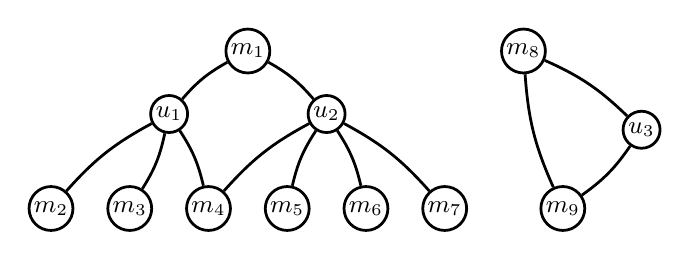
\begin{tikzpicture}[
    every edge/.style={draw, line width=1pt, align=left, sloped}
    ]
  
    \node[draw, circle, inner sep = 1pt, line width=1pt] (m1) at (0, 0) {\small $m_1$};
    \node[draw, circle, inner sep = 1pt, line width=1pt] (u1) at (-1, -0.8) {\small $u_1$};
    \node[draw, circle, inner sep = 1pt, line width=1pt] (u2) at (1, -0.8) {\small $u_2$};
    
    \node[draw, circle, inner sep = 1pt, line width=1pt] (m2) at (-2.5, -2) {\small $m_2$};
    \node[draw, circle, inner sep = 1pt, line width=1pt] (m3) at (-1.5, -2) {\small $m_3$};
    \node[draw, circle, inner sep = 1pt, line width=1pt] (m4) at (-0.5, -2) {\small $m_4$};

    \node[draw, circle, inner sep = 1pt, line width=1pt] (m5) at (0.5, -2) {\small $m_5$};
    \node[draw, circle, inner sep = 1pt, line width=1pt] (m6) at (1.5, -2) {\small $m_6$};
    \node[draw, circle, inner sep = 1pt, line width=1pt] (m7) at (2.5, -2) {\small $m_7$};
  
    \path [-] (m1) edge[bend right=10] node[below=1pt] {} (u1);
    \path [-] (m1) edge[bend left=10] node[below=1pt] {} (u2);

    \path [-] (m2) edge[bend left=10] node[below=1pt] {} (u1);
    \path [-] (m3) edge[bend right=10] node[below=1pt] {} (u1);
    \path [-] (m4) edge[bend right=10] node[below=1pt] {} (u1);
    \path [-] (m4) edge[bend left=10] node[below=1pt] {} (u2);
    
    \path [-] (m5) edge[bend left=10] node[below=1pt] {} (u2);
    \path [-] (m6) edge[bend right=10] node[below=1pt] {} (u2);
    \path [-] (m7) edge[bend right=10] node[below=1pt] {} (u2);


    \node[draw, circle, inner sep = 1pt, line width=1pt] (m8) at (3.5, 0) {\small $m_8$};
    \node[draw, circle, inner sep = 1pt, line width=1pt] (u3) at (5, -1) {\small $u_3$};
    \node[draw, circle, inner sep = 1pt, line width=1pt] (m9) at (4, -2) {\small $m_9$};

    \path [-] (m8) edge[bend right=10] node[below=1pt] {} (m9);
    \path [-] (m9) edge[bend right=10] node[below=1pt] {} (u3);
    \path [-] (m8) edge[bend left=10] node[above=1pt] {} (u3);

  \end{tikzpicture}
  }
  \caption[Example representation of messages.]{
    Example representation of messages. On the left side, 
    messages $m_1$ and $m_4$ share URLs $u_1$ and $u_2$, while $m_2$ only shares $u_1$.
    On the right side, $m_8$ and $m_9$ share or reply one to another, and also share URL $u_3$. 
    Each connected component is a {\em document}.
  }
  \label{fig:model-example}

\end{figure}

% \begin{figure}
%   \centering
%     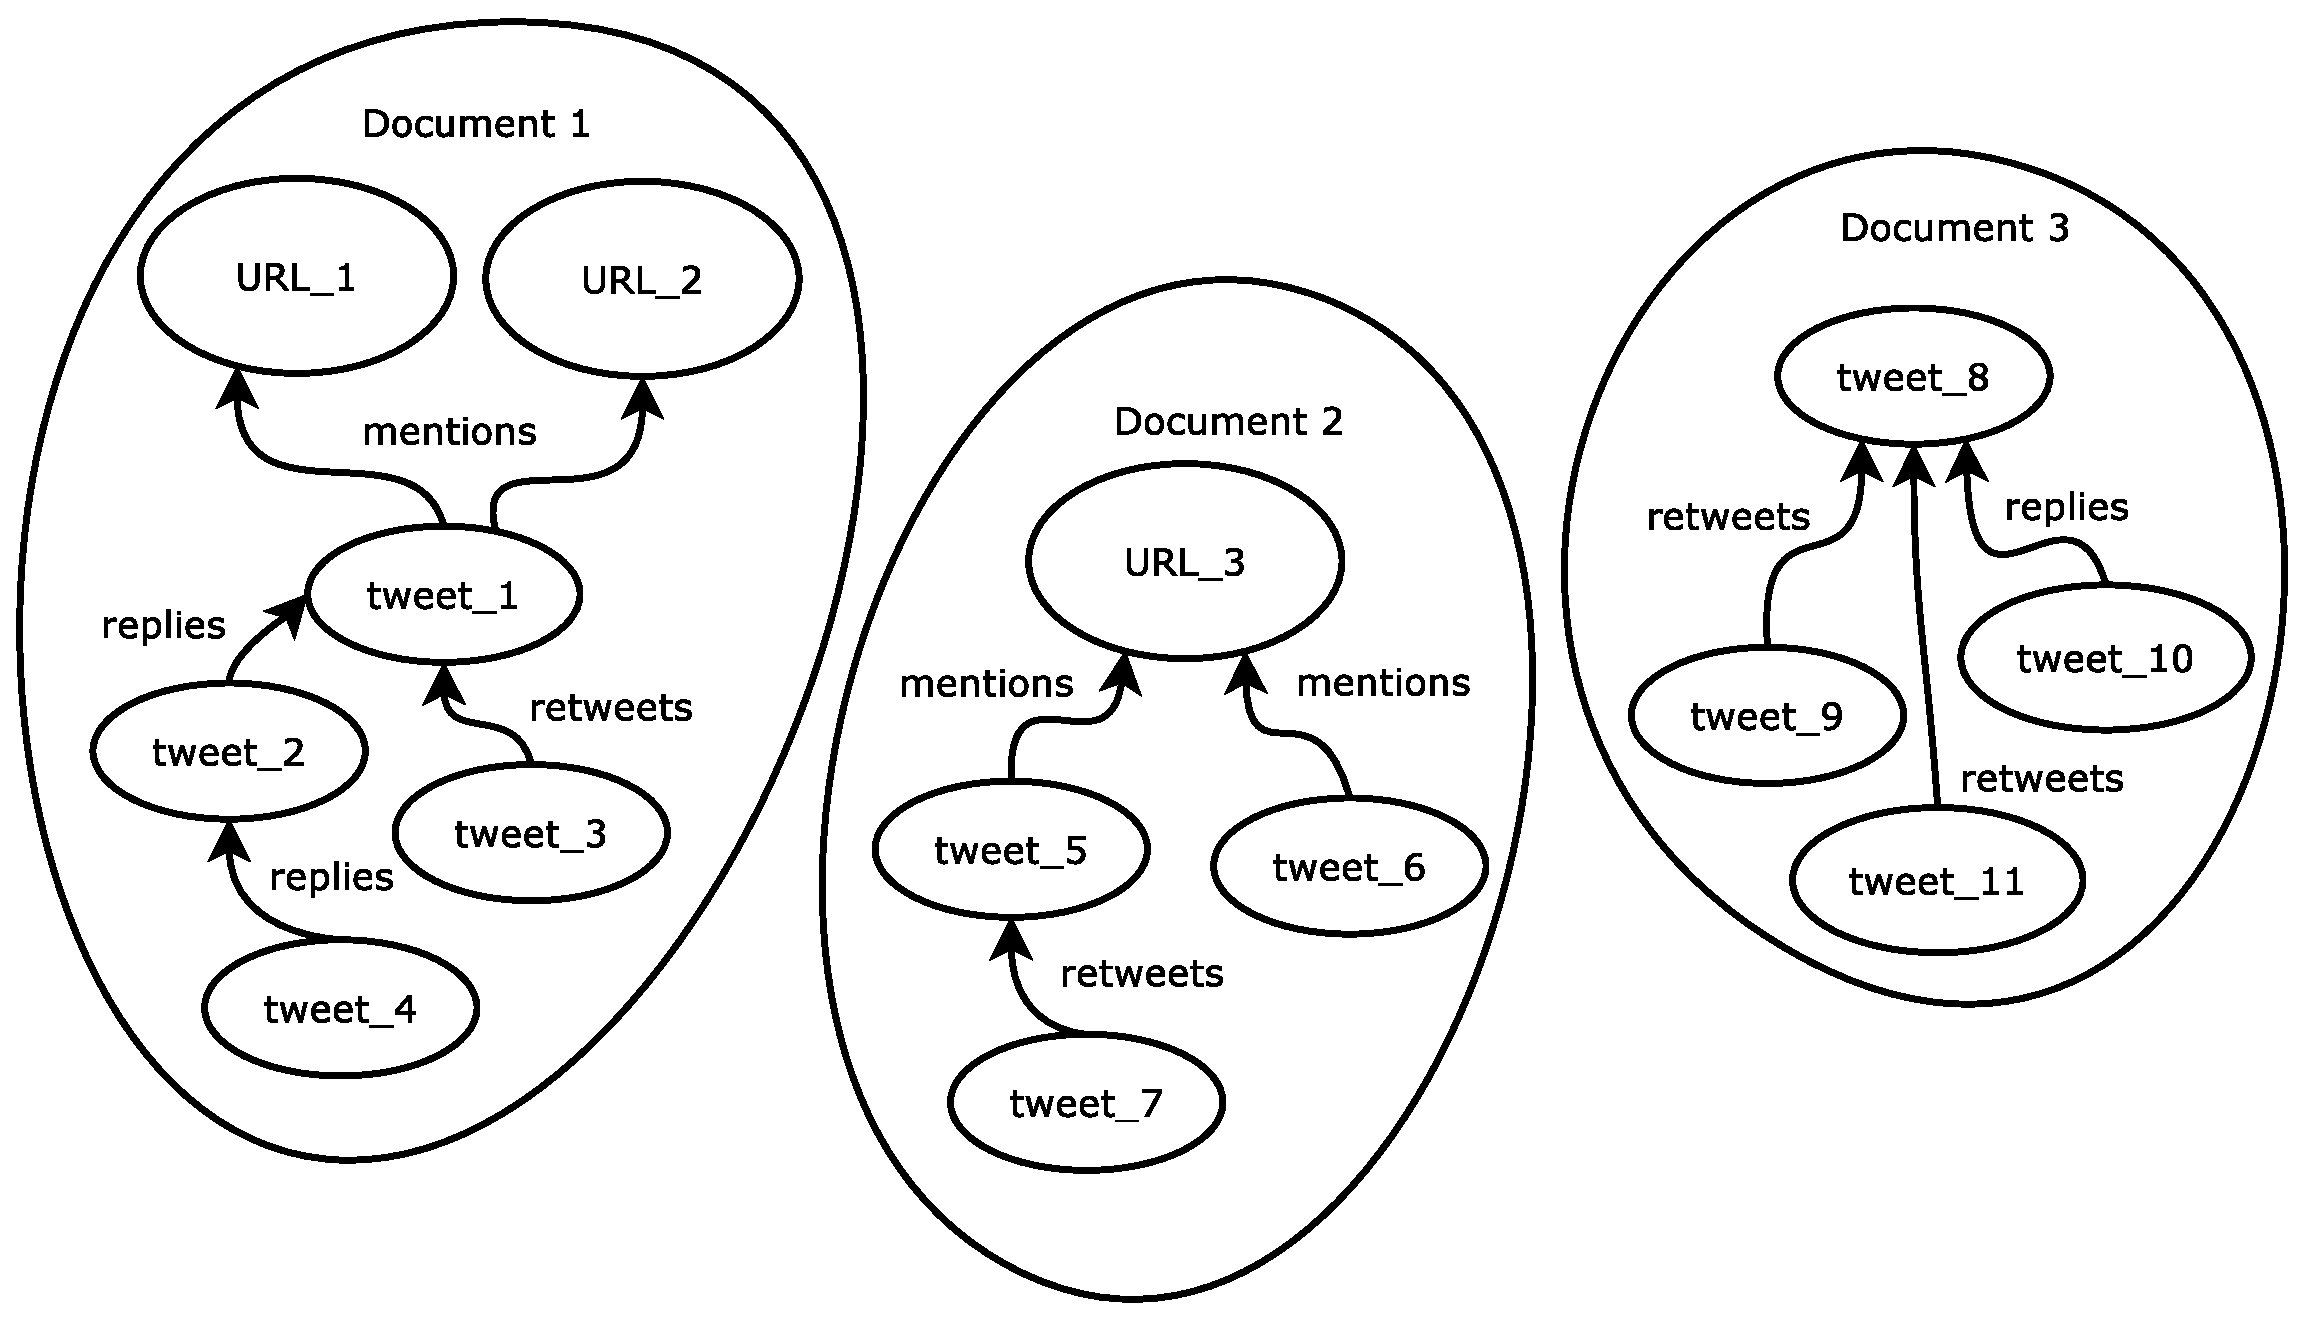
\includegraphics[width=0.4\textwidth]{fig/docs.eps}
%   \caption{Conceptual example of documents. A document is a set of messages that share or reply each other, and the messages that share the same URL. In order to have a representative element for each document, only documents with URL can be considered, and documents with multiple URLs can be duplicated, while each document has a different URL.
%   }\label{fig:model}
% \end{figure}

% Consider Twitter as an example. A document $d$ is a set of URLs, plus the tweets
% that mention those URLs, plus the tweets that retweet or reply any of the
% tweets in $d$. Note that if there are more than one URL, then there should be
% at least one tweet that mention all those URLs, or there is a path of replies
% or retweets between the tweets that mention those URLs individually.
% Figure~\ref{fig:model} shows an example of a few documents.

% \begin{algorithm}
% \caption{Model generation}\label{algo:gen}

% \SetAlgoLined
% \KwData{Messages $T$, URLs $U$ mentioned in messages in $T$}
% \KwResult{Documents $D = \{d_1, d_2, \ldots, d_N\}$, with $d_i\subseteq T\cup U$, for $i\in \{1, \ldots N\}$}
%  $Pairs \leftarrow \emptyset$\;
%  \For{$t \in T$}{
%   \For{$u \in U$ that is mentioned by $t$} {
%     $Pairs \leftarrow Pairs \cup \{(t, u)\}$\;
%   }
%   \If{$\exists t' \in T$ such that $t$ replies to or forwards $t'$}{
%    $Pairs \leftarrow Pairs \cup \{(t, t')\}$\;
%   }
%  }
%  \For{$u \in U$} {
%   \em{UnionFind}.makeSet$(u)$\;
%  }
%  \For{$(p, q) \in Pairs$} {
%   \em{UnionFind}.union$(p, q)$\;
%  }
%  $D \leftarrow UnionFind.sets()$\;
% \end{algorithm}
% \vspace{-0.5cm}

%%%%%%%%%%%%%%%%%%%%%%%%%%%%%%%%%%%%%%%%%%%%%%%%%%%%%%%%%%%%%%%%%%%%%%%%
%%%%%%%%%%%%%%%%%%%%%%%%%%%%%%%%%%%%%%%%%%%%%%%%%%%%%%%%%%%%%%%%%%%%%%%%
%%%%%%%%%%%%%%%%%%%%%%%%%%%%%%%%%%%%%%%%%%%%%%%%%%%%%%%%%%%%%%%%%%%%%%%%
%%%%%%%%%%%%%%%%%%%%%%%%%%%%%%%%%%%%%%%%%%%%%%%%%%%%%%%%%%%%%%%%%%%%%%%%


%\paragraph{\bf{Generation methodology}}\label{sec:methodology}

\subsection*{Methodology for representing events}

Given a set of event-related social media messages, we propose the following
methodology for representation generation:
  
{\bf Filter out generic URLs:} 
%
We call generic URLs (too general with respect to the event) as those that
co-occur with multiple different other URLs across many messages.
%
A URL co-occur with another one URL if they both are shared by the same message.
%
Highly connected URLs are assumed to not contribute information to specific topics: 
links that are very generic (e.g., {\tt cnn.com}) or very general to the event 
(e.g., general reports). 
%
All of the messages mentioning these URLs would fall into the same component,
regardless of their differences in content. 
%
We removed URLs that co-occurred with three or more different URLs across
messages.
%
This threshold yielded the best results in our case studies.


{\bf Representation generation:} 
%
The generation step consists of grouping messages that end up in the same
component, as described in the previous section.
%
For that, a straightforward method is to compute all pairs of messages and pairs
of URLs and messages that fulfill the conditions stated in the representation
definition and then find connected components using a union-find algorithm.
%
The URLs are the non-generic ones identified in the previous step, as an
approximation to the topic-specific URLs.


{\bf Vector representation of documents:} 
%
Finally, we aggregate messages into documents in order to produce a vector
representation, using neural network-based word embeddings.
%
This procedure generates dense document representations.
%
To aggregate messages, we simple compute a vector representation of each word in every message and 
then aggregate all the vectors (for example, using the mean or the sum of all vectors).




% Our goal is to propose a methodology for generating automatic summaries from
% news events on Twitter, exploiting both the multimedia content and the
% importance that users give to certain topics. For that, we learned a
% representation of the URLs shared from event-related tweets (URLs pointing to
% images, videos, other tweets, or other Web pages in general), using the text in
% the tweets that surround those URLs, borrowing the idea of anchor texts in query
% log mining. We used this representation to group the URLs into clusters and then
% used the social features of each tweet in order to rank the URLs and the
% clusters, based on the level of activity that users had on each of those. This
% allowed us to sort the different aspects of an event based on the importance
% that users give to them.



% \subsection{Definitions}

% \paragraph{Tweet} A {em tweet} can be seen as a struct with the following fields:

% \begin{itemize} \item {\em text}: the textual content of the tweet. \item {\em creation\_date}: a
% timestamp when the tweet was published. \item {\em no\_retweets}: the amount of times that tweet was
% shared or       forwarded by other users. \item {\em no\_likes}: the amount of times users ``liked''
% the tweet. \item {\em user}: an identifier of the user who published the tweet. \end{itemize}


% \paragraph{Summary} Given a set of tweets $E = \{t_1, t_2, \ldots, t_N\}$, called an {\em   event},
% we want to select a subset $S \subseteq E$ of tweets, called   a {\em summary}. The summary must
% fulfill the following criteria:

% \begin{itemize}      
% \item {\bf Topical coverage}: the tweets in $S$ must cover the same topics as
% $E$.   \item {\bf Redundancy}: the content of tweets in $S$ must not be redundant with each other.

% \item {\bf Importance}: the tweets in $S$ must be the top $|S|$, with respect to $E$, according to a
% pre-defined ranking function, considering into account the previous two criteria. For example, if
% two tweets have the same value according to the ranking, but     the two of them are equal in terms
% of content, then only one of them should be in $S$.   

% \item {\bf Human-manageable size}: the size of
% $S$ must be of much less size than $E$, only if $E$ is large. {\bf (TODO: define what is ``large''
% and how less is ``less.'')} \end{itemize}

% \paragraph{Replies and retweets} We denote by $\mathit{URL}(t) = \{u_1, u_2, \ldots, u_m\}$ the URLs
% shared by the tweet $t$. $\mathit{URL}(t)$ is empty if $t$ does not share any URL.

% We also denote by $\mathit{replies}(t)$ the set of all tweets $t'$ such that $t'$ is a {\em reply}
% of $t$, or $t'$ is a reply of another tweet in $\mathit{replies}(t)$. The same applies to
% $\mathit{retweets}(t)$, but by considering {\em retweets} instead of replies.

% \paragraph{Document} We now define a {\em document} $d_u$ as a set of tweets, such that those tweets
% share the same URL $u$, plus their replies and retweets, that is,



% Note that a tweet $t$ can be a member of different documents, if $t$ shares more than one URL.


% \subsection{Methodology}

% We make use of the context of multiple tweets in order to arrange them into topically similar
% groups. When a tweet shares an URL $u$, the content of the tweet can be seen as a description (or
% {\em anchor text}) or a comment on the content of $u$. This also applies when a tweet is a {\em
% reply} of another tweet: those two tweets (the reply and the replied) are topically similar, because
% both of them refers to the same subject of discussion. We use this context to group tweets into
% documents.

% Given an event $E$, let $U$ be the set of all the URLs shared across tweets in $E$. The documents
% induced by $U$ are all the subsets of tweets that share at least one URL, $D = \{d_u\ :\ u \in U\}$.
% Our goal is to select representative tweets to create $S$, by using $D$ as a proxy by grouping
% similar tweets into documents.

% One main task is to compare documents. Two documents whose content is topically similar should be
% similar according to the features of its constituents. Note that the documents may have very
% different sizes, and it is possible that two different documents are topically similar. This makes
% comparing documents a difficult task.

% By comparing documents, our goal is to discover sub-topics inside $E$, in order to achieve coverage
% in the resulting summary. Possible implementations for sub-topic identification are clustering (e.g.
% K-Means, K-Medoids, hierarchical, or online/incremental), or process an induced graph from the
% documents (e.g. community detection, connected components, or centrality measures). Another
% alternative, which does not require computing a similarity measure between documents, is the use of
% topic modelling (LDA or Dynamic Topic Models if the time dimension is considered).


% \paragraph{Similarity between documents}

% There are two alternatives when computing similarity between documents:

% \begin{enumerate} \item {\em Consider all the elements of a document as a single element.} For
% example, compute a vector space model (e.g. tf-idf) over the concatenation of tweets in a document
% and then compare the representations using standard cosine similarity. A problem with this approach
% is that diverse content inside a document can be shadowed by the most popular content inside a
% document. Or, on the other hand, if there is a lot of diverse content, then the focus of the
% document can be inaccurate, compared by a smaller, focused document.

% \item {\em Consider each element of a document as a single element.} For example, compare individual
% pairs of tweets of different documents, and then compute an average of similarities to assess the
% similarity of the two documents. This could share a similar problem with the other alternative, as
% diverse content may diffuse the main focus of a document (or be shadowed by the popular content).
% Another alternative is to derive high similarity between unequally-sized documents if {\em some} of
% the tweets in the larger document are {\em very} similar to the tweets in the smaller one.

% Another problem is the sparsity of vocabulary of tweets, if we compare them one by one. But this can
% be settled by using more information about the tweets (for example, by using a word embedding to
% compute similarity between words). \end{enumerate}

% The second approach may be better adjusted to the specific domain, where certain topics of an event
% are way more popular than the rest.

%%%%%% @TODO PONER TABLA CON TWEETS DE EJEMPLOS



\section{Case Studies}
\label{sec:experimental}

We describe the case studies, the data, and the experiment we performed to
validate our representation.

\subsection{Datasets}

%We follow a similar approach to Kalyanam et al.~\cite{kalyanam2016prediction}.
%
We collected tweets using the Twitter Search API using selected news accounts as
seeds for extracting newsworthy search terms.
%
In particular, given a set of verified news accounts in Twitter (such as
BBCNews, CNN, Al Jazeera, etc.), we identify the most common keywords across
their tweets published every hour, and then we use those keywords as search
terms in the Twitter API.
%\footnote{The full list of news accounts is listed in
%\url{https://github.com/mquezada/twitter-event-detection/blob/master/settings.py}}

% The data collection methodology is as follows. 
% %
% Every hour we fetch the latest tweets for each one of the seed accounts. 
% %
% Our assumption is that if an important event is happening in a certain moment
% in time, then several news accounts will be reporting on that event shortly
% after.
% %
% After the removal of stopwords, punctuation, URLs, hashtags, mentions, and
% converting words to lowercase, we tokenize each headline and find named
% entities, such as person names, locations, product names, organizations, etc.
% %
% This is possible due that the selected accounts generally employ formal
% language in their tweets. 
% %
% Then we find common subsets of tokens across the tokenized headlines, using an
% ad-hoc method resembling frequent itemset mining. 
% %
% Finally, from each common subset, we search for more related tweets in the
% Twitter Search API using the top 3 ranked terms for the next hour until the
% next batch of keywords is extracted. 

% The source code of the data collection methodology is
% available\footnote{\url{https://github.com/mquezada/twitter-event-
% detection/}}.
%
For the case studies, we selected three events of different nature, namely a
terrorist attack (2015 Libya Hotel Attack), a long-lasting event (2014 Oscar
Pistorius Trial), and a natural disaster (2015 Nepal Earthquake).
%
Each event has different scales and levels of redundancy. 
%
We report duration in days (corresponding to the amount of days encompassing at
least 95\% of the tweets), total tweets, retweets (with percentage of total
tweets), and unique resolved URLs (Table~\ref{tab:datasets}).
%
We also report some tweets for each event (Table~\ref{tab:sample}).


\begin{table}[ht!]
  \centering
  \caption{Datasets for case studies.}
  \label{tab:datasets}
  \begin{tabular}{@{}lllll@{}}
  \toprule
  Name                  & Duration & Tweets & Retweets & URLs  \\ \midrule Libya
  Hotel Attack    & 8 days   & $28\,616$ & $12\,280$ (43\%)  & $3\,385$
  \\
  Nepal Earthquake      & 1 day   & $522\,434$ & $363\,102$ (70\%) & $22\,661$
  \\ 
  Oscar Pistorius Trial & 70 days  & $113\,189$ & $26\,307$ (23\%)  & $9\,335$
  \\ \bottomrule
  \end{tabular}
\end{table}


% {\bf 2015 Libya Hotel Attack.} 
% %
% In January 27, 2015, a luxury hotel in Tripoli was attacked by men affiliated
% with
% ISIL.\footnote{\url{https://en.wikipedia.org/wiki/2015_Corinthia_Hotel_attack}
% (Accessed: 2019-01-30)}. % Attackers detonated a car bomb outside the hotel, %
% killed security personel and guests, and took hostages afterwards. We filtered
% % our data using keywords such as {\tt libya}, {\tt luxury}, {\tt hotel}, or
% {\tt % attack}. % The tweets ranged from July 2012 to January 27, 2015. The
% existence of % older tweets is explained by the retrieval of retweets and
% older tweets % mentioning the extracted keywords, although more than 95\% of
% the tweets fall % within one week before or at the day of the attack. The
% dataset consists of $28\,604$ tweets (with $12\,280$ or 43\% of them being
% retweets), 25\,683 different short and $3\,385$ unique URLs after expanding
% the short URLs. 
% %
% We found that 5\,759 short URLs were unable to be resolved (due to be
% inaccessible at the time of the resolution).

% % On the other hand, due to the occurrence of keywords such as {\tt luxury}, %
% several unrelated tweets appeared in the dataset, such as the following:

% % \begin{itemize} % \item Cheers {\tt <mention>}, named Best Luxury Hotel in
% The Netherlands by {\tt <mention>}! % \item New York's dazzling Baccarat Hotel
% opens this March, and it looks set to be a corker % \item What are your
% thoughts on this distinctive new hotel planned for development in China? %
% \end{itemize}

% %%

% {\bf 2015 Nepal Earthquake.} 
% %
% In April 25, 2015, Nepal was struck by a 7.8 $\text{M}_\text{W}$ earthquake,
% killing nearly $9\,000$
% people\footnote{\url{https://en.wikipedia.org/wiki/April_2015_Nepal_earthquake}
% (Accessed: 2019-01-30)}. 
% %
% The dataset consists of $522\,434$ tweets, with the 70\% of them being
% retweets.
% %
% Also, $60\,632$ of the short URLs were unable to be resolved.

% %%

% {\bf 2014 Trial of Oscar Pistorius.} 
% %
% The trial of Oscar Pistorius started on March 3, 2014, and in October, 2014 a
% judge sentenced him for a maximum of 5 years for homicide; in 2015 and 2016 he
% received more
% sentences\footnote{\url{https://en.wikipedia.org/wiki/Trial_of_Oscar_Pistorius}
% (Accessed: 2019-01-30)}.
% % 
% The dataset consists of $113\,189$ tweets, with 23\% of them being retweets.
% %
% Also, $21\,807$ short URLs were unable to be resolved.





\subsection{Experimental setting}

To generate the representation for each event, we discarded all tweets that have
more than two URLs or more than three hashtags, as we consider them as
potentially spam tweets. 
%
Note that some spam tweets may not fall into this filter.
%
We resolved every URL mentioned in the resulting tweets by following redirects. 
%
Even though the tweet meta-data may include the URLs as before they were
shortened by the Twitter platform, they are often shortened by additional
external services (e.g., {\tt bit.ly}) even more than once.
%
Also, we removed all query strings from the URLs, with some exceptions, which
for some sites they are relevant to identify the resource (e.g., {\tt ?id=},
{\tt ?fbid=}, {\tt ?v=}, etc.).

%%

The URLs which co-occurred with two or less other URLs in the same tweets were
considered as topic-specific.
%
Then, we computed the representation for each event by identifying connected
components in the graph of tweets and URLs. We discarded tweets without URL.
%
This resulted in $2\,957$ documents for the Libya event, $20\,984$ for the Nepal
event, and $9\,092$ for the Pistorius event.

%%

We used fastText~\cite{bojanowski2016enriching} to produce dense vectors from
the documents.
%
We choose fastText due to its capability to encode sub-word information into the
embeddings and to encode some out-of-vocabulary words, resulting in better
quality embeddings for rare or uncommon words. 
%
This is useful in the context of social media, as there are many words with
misspellings. 
%
For the generation of document vectors, we took all the tweets in a document,
and obtained the vector of each word in each tweet.
%
Then, we took the sum of the vectors of the words in the document.
%
We trained 300-dimension word embeddings using a dataset of 193 million
event-related tweets (3 billion words) using the aforementioned data collection
methodology.
%
Note that the training phase can be done off-line and is done only once.


\subsection{Validation of sub-topic detection task}

To validate our representation in the case studies, we identified topics in our
events using our representation and using raw tweets.
%%

We produced a set of labels from the tweets in order to have a ground truth for
our experiments. 
%
For this, sixteen people (mainly Computer Science undergrad and grad students)
labeled tweets independently using a custom Web interface. 
%
The interface displayed a tweet and a list of labels, and each user could assign
one or more labels to a tweet, mark the tweet as non relevant, or skip it.
%
Some tweets may refer to more than one sub-topic, and we preferred that users
felt free to assign as many labels as they prefer.
%
We imposed a limit of three evaluations per tweet.
%
We manually generated the list of labels using information from news reports in
the Web.
%
The tweets displayed in the interface were chosen in such a way there were
roughly no underrepresented sub-topics.
%
For this, we manually produced a list of keywords for each label, and for each
label ranked the tweets using Okapi BM25 and shuffled the ranked tweets to be
shown in the interface.
%
Finally, to assign the actual label to a tweet, we selected the most voted
label.
%
This resulted in 401 labeled tweets for the Libya event, 368 for Nepal, and 85
for Pistorius.

%%

To find sub-topics, we ran k-means with different number of clusters, using our
representation and raw tweets.
%
For the baseline, we considered each tweet as a document, that is, we computed
the sum of word vectors for each tweet individually.
%
We report normalized mutual information, purity, and entropy for each event,
using the available labels in both settings (Figure~\ref{fig:results}).
%
Note that the measures were done only on the labeled tweets, that is, as if the
unlabeled tweets did not exist in the clustering solution.


%%

We observe that with under our representation, the clustering outperforms the
baseline in some cases. 
%
In the case of the Nepal event, our representation had better purity, NMI and
entropy. 
%
In the case of Pistorius, the measures are very similar. 
%
However, in the case of Libya, our representation matches the baseline after a
certain number of clusters, except in the entropy measure.
%
And in terms of running time, we observed that k-means under the representation
runs one order of magnitude faster than the baseline (Figure~\ref{fig:times}). 
%
These results suggest that our representation is capable of preserving topical
information about the target event, with reduced time required to identify this
kind of information.
 

\begin{figure}
  \centering
  \begin{subfigure}[b]{0.478\textwidth}
      \centering
      \includegraphics[width=\textwidth]{figures/url-model/purity}
      \caption{Purity.}
  \end{subfigure}%

  \begin{subfigure}[b]{0.478\textwidth}
      \centering
      \includegraphics[width=\textwidth]{figures/url-model/nmi} 
      \caption{Normalized Mutual Information.}
  \end{subfigure}

  \begin{subfigure}[b]{0.478\textwidth}
    \centering
    \includegraphics[width=\textwidth]{figures/url-model/entropy} 
    \caption{Entropy.}
  \end{subfigure}

\caption{External clustering measures for target events.}
\label{fig:results}
\end{figure}

\begin{figure}
  \centering
  \includegraphics[width=.478\textwidth]{figures/url-model/times}
  \caption{Running times for clustering.}\label{fig:times}
\end{figure}%

\section{Discussion and Future Work}\label{sec:conclusions}

% % In this paper, we presented a lightweight representation to represent newsworthy
% information in social media, and a methodology to generate a representation from
% a set of social media messages.
% %
% Our representation leverages the use of shared URLs in the context of news
% events to aggregate common information across messages.
% %
% We observed that our representation is capable to preserve topical information
% of an event.
% %
% At the same time, it is suitable to be significantly smaller than the original
% dataset, requiring much less computational resources to perform standard tasks.
% %
% This representation requires little data preprocessing, meaning that is
% convenient to use in an scenario of having large, raw, uncurated data.
%%
% In a future work, we are interested in studying new strategies to represent
% external URLs using social media data, and how this can be used to better
% understand real-world events.

Our proposed representation allows us to identify sub-topics in an event much
faster than traditional or off-the-self methods.
%
However, there is room for improvement in terms of the results.
%
For this, we need to perform a large scale evaluation, although it is hard to
find ground truth data for large, raw, uncurated social media
messages~\cite{Alonso:2015:WCW:2740908.2745397}.
%
For this case scenario, our methodology aims to help processing large quantities
of noisy, uncurated data around news events more effectively.
%
In a future work, we are interested in studying new strategies to represent
external URLs using social media data, and how this can be used to better
understand real-world events.
%
For example, to study how these signals, such as URL sharing in social media,
can give us clues about the development of critical events, such as natural
disasters or breaking news.


\chapter{Conclusions}

In this dissertation we have proposed different representations of news events
from social media data.
%
Along with each representation, we also implemented some applications, showing
the effectiveness and usefulness of the representations.

\section{Summary of Contributions}

\paragraph{Model of User Reaction.}
%
We proposed an event representation that allows us to model events based on the
level of activity of users in relation to news events. 
%
This model is based on the learned distribution of inter-arrival rates of social
media posts.
%
Using a dataset of about five thousand news events obtained from Twitter, we
computed the most frequent inter-arrival times of tweets, and used them to create
a vector representation of events based on these rates.
%
This means that our model is independent of the scale of the event.
%
We characterized the high-activity and low-activity events separately, finding
statistically significant differences between event types.
%
We also showed that other event features, such as the ratio of retweets or the
amount of words in the messages, are predictors of the level of activity of an
event, and that this level is very identifiable at early stages of the event.
%
The idea behind this representation was to model the impact that events cause in
the community, unlike notions such as virality, which is applicable to memes or
units of information, or popularity, which accounts for large-scale events.

\paragraph{Model of Spatio-Temporal Context.}
%
In a similar fashion, we proposed an event representation aiming for another way
to measure the impact of the occurrence, in this case, based on the locations
from where users comment on the news, and the locations where the event
happened.
%
This allows us to explore how different locations are affected by different
events, and how users from different locations are interested in those events.
%
To show the effectiveness of this representation, we made an exploratory
analysis of a 2-year dataset of news events from Twitter, encompassing about
25,000 events, showing connections between locations and insights about
international relations using tweets.

\paragraph{Model of Aggregated Content.}
%
Lastly, we proposed a representation of content of news events, leveraging the
redundancy of information and the evidence that users share URLs when exposed to
a news event.
%
Our methodology generates a compact representation of events, allowing us to
perform standard tasks using less data, with similar results.
%
We showed how our representation could be used to find sub-topics in events,
comparing the sub-topics with those obtained by using all the data.
%
In our preliminary experiments, we showed that our model yields similar
clustering metrics compared to the complete data, while using one order of
magnitude fewer vectors.


With respect to the thesis statement, we can say that the use of different types
of context information, such as the user reaction, the spatio-temporal setting
of the events, or the use of implicit information, such as the occurrence of
shared URLs, are {\em novel} and {\em effective} to perform analysis of news events. 
%
For instance, we observed that it is possible to determine if a news event is
going to produce high levels of activity in the community, meaning that there
are implicit signals given by the community as a whole, and not necessarily in
individual posts.
%
On the other hand, the modeling of the spatio-temporal context allows us to
infer new relationships between geopolitical entities (e.g., countries) using
social media data.
%
In the long run it can serve as a repository of historical data for further
analysis of political or societal trends\footnote{Consider, for example, the
applications to Comparative Historical Research.
\url{https://en.wikipedia.org/wiki/Comparative_historical_research} (Accessed:
August 24, 2019).}.
%
Finally, we showed a preliminary study of the potential of aggregating
information based on shared content, in this case about shared URLs.
%
The ability of posts to preserve topical information when aggregated by the same
shared URLs can be useful, for instance, to generate automatic summaries of
events, contributing to the possibility of storing this information for posterior
analyses.




\section{Limitations and Future Directions}

Future work involves some of the limitations of our work, such as the quality of
our data collection methodology, the limitations regarding the evaluation, the
capabilities of our models to be transferable to other social media platforms
besides Twitter, and the steps we need to perform to deal with biased data.

\subsection*{Data Collection}
% DATA
One of the future directions is related to the data extraction methodology
described in Chapter~\ref{chapter:data}. 
%
The news event extraction methodology relies on the headlines published by news
media accounts. 
%
This technique provides good precision in terms of reporting events that did in
fact exist in the real-world, but might omit informative events that did not
receive media coverage (unknown recall).
%
Therefore, the current data extraction approach can fail to retrieve events such
as citizen movements and other important events that were reported only via
social networks.  
%
In addition, in the current data extraction setup the initial seeds for the
event collection came from a reduced list of news media accounts, with limited
country coverage and languages.
%
Although the news event dataset likely represents a great majority of the news
events and related tweets posted on Twitter, the collection will miss the long
tail of events that had impact in other less represented countries worldwide. 
%
We note that there are several ways in which this bias can be mitigated in the
future, all of them related to replacing external modules in the data input
phase of the framework.
%
Another direction regarding this issue corresponds to merging events that
discuss the same news topic in different languages. 
%
Recent approaches in cross-language microblogging retrieval
\cite{Godavarthy2016} can be integrated for news event retrieval within our
framework.
%
Also, we will consider the possibility of incorporating higher-level temporal
properties of events, such as if the event is long-term, punctual or recurring,
as defined in the work of Tan et al.~\cite{st-model_2009}.


\subsection*{Evaluation}

There is a limited amount of annotated datasets or ground-truths to perform
evaluation in the context of social media data.
%
In particular, one of the reasons is the high volume of posts being
published every moment.
%
Everyday posts contain little information due to their extension, are redundant
(possibly re-sharing other posts), it is difficult to assign categorical
labels from the content of the posts, etc.
%
Besides, new tasks or goals require new types of ground-truths, which may not be
available at the moment.

In our setting, {\em high-level analysis of news events} is not a well-defined
task.
%
For instance, our spatio-temporal context representation
(Chapter~\ref{chapter:geopolitical}) serves as a model for data exploration or
international relations based on shared newsworthy posts, which depends on the
quality of other tools (e.g., toponym extraction and annotation) and it is not
directly evaluated against alternative representations.
%
This is a limitation of our proposal, and it is required for future works to
assess the quality of the representation.
%
On the other hand, our content-based event representation
(Chapter~\ref{chapter:url}) leveraged redundant posts in order to extract a
useful and compact representation to perform data exploration or topic
detection.
%
In this case, relevant ground-truths were clean and pre-processed 
datasets~\cite{ICWSM1817816}, without duplicate posts, making our validation not
useful in that context.
%
For that reason we carried out our validation on manually labeled un-curated
datasets.



\subsection*{Generalization Potential in other Platforms}
% TRANSFERABILITY
In addition, we note that although our proposed event representations can be
considered generalizable to other social media platforms, we have not validated
it on other sources of information besides Twitter. 
%
It is not certain that for other social media platforms we will have enough
information, regarding user location and data availability, in order to produce
accurate event representations.
%
For example, it is possible to obtain similar results regarding the detection of
high-activity events, or the same topical results when aggregating content by
the same shared URLs?


\subsection*{Veracity and Ethics}
%
Having more data or the possibility to explore different platforms involve new
problems, such as the assessment of the veracity of the information.
%
In this work we did not tackle this issue, assuming that all the events in our
dataset are trustworthy.
%
That means, that every event in our dataset corresponds to a real-world
occurrence covered by recognized news outlets.
%
However, we cannot ensure that these outlets were reporting trustworthy
information, and that users were posting misled information.
%
This problem raised an entire line of research over recent
years~\cite{10.1145/3137597.3137600,bovet2019influence,10.5555/2893873.2893884,10.1145/1835449.1835522,benevenuto2010detecting,10.1145/1920261.1920263}.
%
In this work we employed simple measures on the data, such as the removal of
tweets that share multiple URLs or hashtags, although specialized techniques
could be applied.
%
This is a limitation that could affect our results throughout this work,
notwithstanding that in the case of having fabricated content in our dataset,
its impact in our results requires further investigation.
%
For instance, we anecdotally observed during the development of the
representation presented in Chapter~\ref{chapter:url} that the URL graph was
easily capable of partition the Libya event into two clusters:
occurrence-related content (regarding the attack mentioned in the event), and
unrelated content, such as advertising for luxury hotels in Libya.


Similar to this problem is the bias in the social platforms and the gathered
data.
%
We already performed some data normalization (e.g., in
Chapter~\ref{chapter:geopolitical}, we normalized the amount of messages in
order to avoid certain countries being over-represented), however, there are
implicit biases or biases that are dependent on demographic information, such as
age or gender~\cite{Graells-Garrido:2019:RAD:3292522.3326057}.
%
No platform is representative of the population, hence we need to incorporate a
sound methodology for normalizing data and be aware of the consequences of
polarization, bias, and misinformation present in social media data.

% \input{glosario.tex} % opcional

\bibliographystyle{plain}
\bibliography{bibliografia}

\begin{appendix}
% \pagestyle{fancy}
% \fancyhf{}
% \lhead{APPENDIX \thechapter}
% \rhead{\rightmark}
% \cfoot{\thepage}

\chapter{List of News Sources for Data Collection}\label{ape:news}

The following table lists the news sources used for retrieving news
events from Twitter. The first column corresponds to the account name
(it can be accessed in a browser
in \url{http://twitter.com/accountname}), while the second and third
column correspond to the data from each account's Twitter page.

\begin{longtable}{l|l|l}
\hline
\textbf{Twitter Account} & \textbf{Name} & \textbf{Location} \\
\hline
\endfirsthead
\multicolumn{3}{l}%
{\tablename\ \thetable\ -- \textit{Continued from previous page}} \\
\hline
\textbf{Twitter Account} & \textbf{Name} & \textbf{Location} \\
\hline
\endhead
\hline \multicolumn{3}{l}{\textit{Continued on next page}} \\
\endfoot
\hline
\endlastfoot

 breakingnews     &  Breaking News         &  Global                      \\
 cnnbrk           &  CNN Breaking News     &  Everywhere                  \\
 cnn              &  CNN                   &                              \\
 nytimes          &  The New York Times    &  New York City               \\
 bbcbreaking      &  BBC Breaking News     &  London, UK                  \\
 theeconomist     &  The Economist         &  London                      \\
 skynewsbreak     &  Sky News Newsdesk     &  London, UK                  \\
 reuters          &  Reuters Top News      &  Around the world            \\
 wsjbreakingnews  &  WSJ Breaking News     &  New York, NY                \\
 foxnews          &  Fox News              &  U.S.A.                      \\
 msnbc\_breaking   &  msnbc.com Breaking    &                              \\
 skynews          &  Sky News              &  London, UK                  \\
 nbcnews          &  NBC News              &  New York, NY                \\
 cbsnews          &  CBS News              &  New York, NY                \\
 bbcworld         &  BBC News (World)      &  London, UK                  \\
 abc              &  ABC News              &  New York, NY                \\
 bbcnews          &  BBC News (UK)         &  London                      \\
 ap               &  The Associated Press  &  Global                      \\
 telegraphnews    &  Telegraph News        &  London, UK                  \\
 breakingnewsuk   &  Breaking News UK      &  London                      \\
 channel4news     &  Channel 4 News        &  Weekdays at 7 on Channel 4  \\
 twcbreaking      &  TWC Breaking          &  Atlanta, GA                 \\
 washingtonpost   &  Washington Post       &  Washington, D.C.            \\
 yahoonews        &  Yahoo News            &  Santa Monica, Calif.        \\
 breakingpol      &  Breaking Politics     &  Global                      \\
 nydailynews      &  New York Daily News   &  New York City               \\
 ajenglish        &  Al Jazeera English    &  Doha, Qatar                 \\
 usatoday         &  USA TODAY             &  USA TODAY HQ, McLean, Va.   \\
 wsj              &  Wall Street Journal   &  New York, NY                \\
 guardiannews     &  Guardian news         &  London                      \\
 bloombergnews    &  Bloomberg News        &  New York and the World      \\
 abcworldnews     &  ABC World News        &  New York                    \\
 nypost           &  New York Post         &  New York, NY                \\
 msnbc            &  msnbc                 &                              \\
 nbcnightlynews   &  NBC Nightly News      &  New York                    \\
 huffingtonpost   &  Huffington Post       &                              \\
 rt\_com           &  RT                    &                              \\
 abcnews          &  ABC News              &  Australia                   \\
 latimes          &  Los Angeles Times     &  Los Angeles, CA             \\
 googlenews       &  Google News           &  Mountain View, CA           \\
 cnnlive          &  CNN Live              &  Everywhere                  \\
 newshour         &  NewsHour              &  Arlington, VA               \\
 guardian         &  The Guardian          &  London                      \\
 afp              &  Agence France-Presse  &  France                      \\
 independent      &  The Independent       &  London, United Kingdom      \\
 ndtv             &  NDTV                  &  India                       \\
 cp24             &  CP24                  &  Toronto                     \\
 reuterslive      &  Reuters Live          &  Global                      \\
 bostonglobe      &  The Boston Globe      &  Boston, MA                  \\
 foxnewsalert     &  Fox News Alert        &  New York, NY                \\
 ft               &  Financial Times       &  London                      \\
 jerusalem\_post   &  The Jerusalem Post    &  Israel                      \\
 bbcnewsus        &  BBC News US           &  Washington DC               \\
 foxheadlines     &  Fox News              &  New York, NY                \\
 forbes           &  Forbes                &  New York, NY                \\
 thetimes         &  The Times of London   &  London                      \\
 usnews           &  U.S. News             &  Washington, DC\\


\caption[List of news accounts.]{List of news account. The first
  column is the Twitter account. It can be accessed in a browser in
  \texttt{http://twitter.com/accountname}. The second and third column
  data was obtained from each account's page.}

\end{longtable}



\clearpage

\end{appendix} % opcionales

\listoftodos[Notes]  % TODO QUITAR ESTA LISTA !

\end{document}
